%%%%%%%%%%%%%%%%%%%%%%%%%%%%%%%%%%%%%%%%%
% Masters/Doctoral Thesis 
% LaTeX Template
% Version 2.5 (27/8/17)
%
% This template was downloaded from:
% http://www.LaTeXTemplates.com
%
% Version 2.x major modifications by:
% Vel (vel@latextemplates.com)
%
% This template is based on a template by:
% Steve Gunn (http://users.ecs.soton.ac.uk/srg/softwaretools/document/templates/)
% Sunil Patel (http://www.sunilpatel.co.uk/thesis-template/)
%
% Template license:
% CC BY-NC-SA 3.0 (http://creativecommons.org/licenses/by-nc-sa/3.0/)
%
%%%%%%%%%%%%%%%%%%%%%%%%%%%%%%%%%%%%%%%%%

%----------------------------------------------------------------------------------------
%	PACKAGES AND OTHER DOCUMENT CONFIGURATIONS
%----------------------------------------------------------------------------------------

\documentclass[
11pt, % The default document font size, options: 10pt, 11pt, 12pt
%oneside, % Two side (alternating margins) for binding by default, uncomment to switch to one side
english, % ngerman for German
singlespacing, % Single line spacing, alternatives: onehalfspacing or doublespacing
%draft, % Uncomment to enable draft mode (no pictures, no links, overfull hboxes indicated)
%nolistspacing, % If the document is onehalfspacing or doublespacing, uncomment this to set spacing in lists to single
%liststotoc, % Uncomment to add the list of figures/tables/etc to the table of contents
%toctotoc, % Uncomment to add the main table of contents to the table of contents
%parskip, % Uncomment to add space between paragraphs
%nohyperref, % Uncomment to not load the hyperref package
headsepline, % Uncomment to get a line under the header
%chapterinoneline, % Uncomment to place the chapter title next to the number on one line
%consistentlayout, % Uncomment to change the layout of the declaration, abstract and acknowledgements pages to match the default layout
]{MastersDoctoralThesis} % The class file specifying the document structure

\usepackage[utf8]{inputenc} % Required for inputting international characters
\usepackage[T1]{fontenc} % Output font encoding for international characters

\usepackage{mathpazo} % Use the Palatino font by default

\usepackage[backend=bibtex,style=numeric,natbib=true]{biblatex} % Use the bibtex backend with the authoryear citation style (which resembles APA)

\addbibresource{example.bib} % The filename of the bibliography

\usepackage[autostyle=true]{csquotes} % Required to generate language-dependent quotes in the bibliography

%----------------------------------------------------------------------------------------
%	MARGIN SETTINGS
%----------------------------------------------------------------------------------------

\geometry{
	paper=a4paper, % Change to letterpaper for US letter
	inner=2.5cm, % Inner margin
	outer=3.8cm, % Outer margin
	bindingoffset=.5cm, % Binding offset
	top=1.5cm, % Top margin
	bottom=1.5cm, % Bottom margin
	%showframe, % Uncomment to show how the type block is set on the page
}

%----------------------------------------------------------------------------------------
%	THESIS INFORMATION
%----------------------------------------------------------------------------------------

\thesistitle{Thesis Title} % Your thesis title, this is used in the title and abstract, print it elsewhere with \ttitle
\supervisor{Dr. James \textsc{Smith}} % Your supervisor's name, this is used in the title page, print it elsewhere with \supname
\examiner{} % Your examiner's name, this is not currently used anywhere in the template, print it elsewhere with \examname
\degree{Doctor of Philosophy} % Your degree name, this is used in the title page and abstract, print it elsewhere with \degreename
\author{John \textsc{Smith}} % Your name, this is used in the title page and abstract, print it elsewhere with \authorname
\addresses{} % Your address, this is not currently used anywhere in the template, print it elsewhere with \addressname

\subject{Biological Sciences} % Your subject area, this is not currently used anywhere in the template, print it elsewhere with \subjectname
\keywords{} % Keywords for your thesis, this is not currently used anywhere in the template, print it elsewhere with \keywordnames
\university{\href{http://www.university.com}{University Name}} % Your university's name and URL, this is used in the title page and abstract, print it elsewhere with \univname
\department{\href{http://department.university.com}{Department or School Name}} % Your department's name and URL, this is used in the title page and abstract, print it elsewhere with \deptname
\group{\href{http://researchgroup.university.com}{Research Group Name}} % Your research group's name and URL, this is used in the title page, print it elsewhere with \groupname
\faculty{\href{http://faculty.university.com}{Faculty Name}} % Your faculty's name and URL, this is used in the title page and abstract, print it elsewhere with \facname

\AtBeginDocument{
\hypersetup{pdftitle=\ttitle} % Set the PDF's title to your title
\hypersetup{pdfauthor=\authorname} % Set the PDF's author to your name
\hypersetup{pdfkeywords=\keywordnames} % Set the PDF's keywords to your keywords
}

\begin{document}

\frontmatter % Use roman page numbering style (i, ii, iii, iv...) for the pre-content pages

\pagestyle{plain} % Default to the plain heading style until the thesis style is called for the body content

%----------------------------------------------------------------------------------------
%	TITLE PAGE
%----------------------------------------------------------------------------------------

\begin{titlepage}
\begin{center}

\vspace*{.06\textheight}
{\scshape\LARGE \univname\par}\vspace{1.5cm} % University name
\textsc{\Large Doctoral Thesis}\\[0.5cm] % Thesis type

\HRule \\[0.4cm] % Horizontal line
{\huge \bfseries \ttitle\par}\vspace{0.4cm} % Thesis title
\HRule \\[1.5cm] % Horizontal line
 
\begin{minipage}[t]{0.4\textwidth}
\begin{flushleft} \large
\emph{Author:}\\
\href{http://www.johnsmith.com}{\authorname} % Author name - remove the \href bracket to remove the link
\end{flushleft}
\end{minipage}
\begin{minipage}[t]{0.4\textwidth}
\begin{flushright} \large
\emph{Supervisor:} \\
\href{http://www.jamessmith.com}{\supname} % Supervisor name - remove the \href bracket to remove the link  
\end{flushright}
\end{minipage}\\[3cm]
 
\vfill

\large \textit{A thesis submitted in fulfillment of the requirements\\ for the degree of \degreename}\\[0.3cm] % University requirement text
\textit{in the}\\[0.4cm]
\groupname\\\deptname\\[2cm] % Research group name and department name
 
\vfill

{\large \today}\\[4cm] % Date
%\includegraphics{Logo} % University/department logo - uncomment to place it
 
\vfill
\end{center}
\end{titlepage}

%----------------------------------------------------------------------------------------
%	DECLARATION PAGE
%----------------------------------------------------------------------------------------

\begin{declaration}
\addchaptertocentry{\authorshipname} % Add the declaration to the table of contents
\noindent I, \authorname, declare that this thesis titled, \enquote{\ttitle} and the work presented in it are my own. I confirm that:

\begin{itemize} 
\item This work was done wholly or mainly while in candidature for a research degree at this University.
\item Where any part of this thesis has previously been submitted for a degree or any other qualification at this University or any other institution, this has been clearly stated.
\item Where I have consulted the published work of others, this is always clearly attributed.
\item Where I have quoted from the work of others, the source is always given. With the exception of such quotations, this thesis is entirely my own work.
\item I have acknowledged all main sources of help.
\item Where the thesis is based on work done by myself jointly with others, I have made clear exactly what was done by others and what I have contributed myself.\\
\end{itemize}
 
\noindent Signed:\\
\rule[0.5em]{25em}{0.5pt} % This prints a line for the signature
 
\noindent Date:\\
\rule[0.5em]{25em}{0.5pt} % This prints a line to write the date
\end{declaration}

\cleardoublepage

%----------------------------------------------------------------------------------------
%	QUOTATION PAGE
%----------------------------------------------------------------------------------------

\vspace*{0.2\textheight}

\noindent\enquote{\itshape Thanks to my solid academic training, today I can write hundreds of words on virtually any topic without possessing a shred of information, which is how I got a good job in journalism.}\bigbreak

\hfill Dave Barry

%----------------------------------------------------------------------------------------
%	ABSTRACT PAGE
%----------------------------------------------------------------------------------------

\begin{abstract}
\addchaptertocentry{\abstractname} % Add the abstract to the table of contents
The Thesis Abstract is written here (and usually kept to just this page). The page is kept centered vertically so can expand into the blank space above the title too\ldots
\end{abstract}

%----------------------------------------------------------------------------------------
%	ACKNOWLEDGEMENTS
%----------------------------------------------------------------------------------------

\begin{acknowledgements}
\addchaptertocentry{\acknowledgementname} % Add the acknowledgements to the table of contents
The acknowledgments and the people to thank go here, don't forget to include your project advisor\ldots
\end{acknowledgements}

%----------------------------------------------------------------------------------------
%	LIST OF CONTENTS/FIGURES/TABLES PAGES
%----------------------------------------------------------------------------------------

\tableofcontents % Prints the main table of contents

\listoffigures % Prints the list of figures

\listoftables % Prints the list of tables



%----------------------------------------------------------------------------------------

%----------------------------------------------------------------------------------------
%	THESIS CONTENT - CHAPTERS
%----------------------------------------------------------------------------------------

\mainmatter % Begin numeric (1,2,3...) page numbering

\pagestyle{thesis} % Return the page headers back to the "thesis" style

% Include the chapters of the thesis as separate files from the Chapters folder
% Uncomment the lines as you write the chapters

% Chapter 1

\chapter{Introduction} % Main chapter title

\label{Introduction} % For referencing the chapter elsewhere, use \ref{Chapter1} 

%----------------------------------------------------------------------------------------

% Define some commands to keep the formatting separated from the content 
% Define some commands to keep the formatting separated from the content 
\newcommand{\keyword}[1]{\textbf{#1}}
\newcommand{\tabhead}[1]{\textbf{#1}}
\newcommand{\code}[1]{\texttt{#1}}
\newcommand{\file}[1]{\texttt{\bfseries#1}}
\newcommand{\option}[1]{\texttt{\itshape#1}}

%----------------------------------------------------------------------------------------


This master thesis has been completed for the Department of Design Sciences at Lund University in collaboration with the company Tetra pak. This first chapter will introduce the background, purpose and scope.

\section{Background}
Working in Shanghai for a summer I noticed that there was a big difference in how Chinese websites where designed compared to western sites. I found the Chinese sites very overwhelming in information density. I assumed that this was because of a simple difference in cultural trends. Later I came across some cross-cultural research articles proving that there is a difference in how people in western and eastern societies perceive information. Does this also influence how the Chinese web pages are designed? Together with Tetra pak, this thesis project is created to examine the differences in web design in eastern and western cultures and to find out if a global interface for both cultures can be created.

\section{Global Website design}
Designing websites for a global market are something that is becoming more and more necessary for larger companies to do. In spite of the need and popularity of global designed websites not much research has been made in this field for user experience. Many companies simply try to launch their local product globally and hope the design work everywhere. Some companies simply create a new product for the different market without researching if this is necessary or not. It is clear that websites look different in cultures all over the world. But how much of this difference is because of cultural trends? Are parts of these websites been designed after a difference in how the culture perceive information? How well can do users from different cultures perform on different web elements?

There is a surprising lack of research done on this subject, despite this, companies all over the world spend millions trying to build information products for cultures without the least bit of knowledge about how the users from that culture perceive information. There are a quite a few assumptions that are usually made about users in different cultures. The first and most common assumption is that all users process information the same way. This is proven to not be the case despite this most people believe that the differences in web layout are mostly due to a difference in language or due to a trend. The second assumption is that because eastern websites are designed differently the users there prefer this type of design, or this type of design is more suitable for users of that culture since it is what they are used to. There are quite a lot of unclarities when examining web pages and web apps in different cultures and hopefully, this thesis will resolve some of these unclarities.

\section{Tetra Pak}

\section{Limitations}

\section{Purpose}
The purpose of this thesis is to research the differences between western and eastern website usage, and how differences in perception plays a role in this. To do this we will try to answer the following questions:
 \begin{enumerate}
	\item Are differences in interface design due to differences in information processing styles or trends?
	\item Do different processing styles in Western (analytical) versus Chinese (holistic) users significantly affect performance on different interfaces?
	\item Can one Global interface be created, or should web designers focus on creating separate user interfaces for different cultures?
\end{enumerate}

Tetra pak is a global company that is 
		

\section{scope}
Focus on diffrences between china and sweden



% Chapter 1

\chapter{Theory} % Main chapter title

\label{Theory} % For referencing the chapter elsewhere, use \ref{Chapter1} 

%----------------------------------------------------------------------------------------



%----------------------------------------------------------------------------------------
\section{Cultural differences in Perception}
Cultural differences affect more than just how consumers behave, it also affects how users perceive information. According to (bla and bla) "good quote" \cite{Holistic_vs_Analytic}
\section{User Centred design}
\section{Usability}
\section{User Experience}
User Experience (UX) is an expression popularised by Donald Norman and Jakob Nielsen in "The design of everyday things" (länka på rätt sätt)(Källa!). Norman and Nielsen define User Experience in the following way “True user experience goes far beyond giving customers what they say they want, or providing checklist features. In order to achieve high-quality user experience in a company’s offerings there must be a seamless merging of the services of multiple disciplines, including engineering, marketing, graphical and industrial design, and interface design” (Norman and Nielsen, 2016). (latex quota på rätt sätt). 
\\\\
The term "User Experience" is a widely applied term in web design and it is associated with a multitude of definitions. The International Organization for Standardization (ISO) has also attempted to define the term. Specifically, the organization, in ISO 9241-210, defines UX as “A person's perceptions and responses that result from the use and/or anticipated use of a product, system or service.” Further, the ISO states that “UX includes all users' emotions, beliefs, preferences, perceptions, physical and psychological responses, behaviours and accomplishments that occur before, during and after use”. The standard also states that “UX is a consequence of functionality, system performance, interactive behaviour and assistive capabilities of the interactive system, the user's internal and physical state resulting from prior brand image, presentation, experiences, attitudes, skills and personality, and the context of use” (dubbel kolla att detta kanske är för kopierat?)


\section{Elements of Web Design}
\section{F-shaped Pattern}
The F-shaped pattern refers to findings made in a study on user eye movements  \cite{pernice2014people} (find correct article for f-shaped pattern and cite it here as well). This pattern has been dubbed the "F-shaped pattern" since the study found that users often scan through pages starting with a horizontal movement, usually across the upper part of the content area. Users then tend to read across in a second horizontal movement further down on the page that typically spans a shorter area. Lastly, users scan the content’s left side in a vertical movement. When measuring users' eye gazing as a heat map, this creates a pattern that resembles an F. Web developers, either knowingly or unknowingly, often design their websites according to this pattern. The F-shaped pattern is not an absolute law and several other scanning patterns exist, but the F-shaped pattern remains the most prevalent in western cultures. \cite{f-shape_today} If a developer designs a page without knowledge about this pattern, they risk putting important information in places where users might miss it. The F-shaped pattern is mostly prevalent in western cultures, where the studies have been conducted.

\section{Perception in asia (f-shaped pattern.)}

\section{Natural Mapping}
\section{User Testing}

\section{Usability Metrics}
There are several different types of metrics that can be used to measure the usability of a prototype or product. Among these metrics are performance metrics, Issues-based metrics, self-reported metrics, behavioral metrics, comparative metrics, and etc \cite{tullis_albert_2011}. For this project, we have decided to focus on performance metrics and self-reported metrics. Usability metrics are powerful tools that are generally under utilized by most companies \cite{norman_metrics}. 
\subsection{Performance Metrics}
Performance metrics can be used to measure a user's behavior when interacting with a product. In this project, the performance metric data will automatically be gathered and sent to a database. This data will then be further analyzed to gain a deeper understanding of how the users engage with the product. (DOUBLE CHECK ->)To be statistically significant the data gathered with a appropriate confidentiality interval at least eight participants are needed \cite{tullis_albert_2011}.(<- DOUBLE CHECK)

 There are 5 basic performance metrics which include: \cite{tullis_albert_2011} \begin{itemize}
\item Task success
\item Time-on-task
\item Errors
\item Efficiency
\item Learnability
\end{itemize}
In order to measure the task rate success metric, the required task must be clearly defined and have an unambiguous goal. For example, "send an email to person x" reflects a well structured task, thus, task success rate can be accurately measured given the well-defined objective. Conversely, the task, "research budget car brands" does not offer clear guidelines and can be responded to in multitude of ways due to its ill-defined objective and, as such, would not be suitable for measuring task success. There are two types of task success forms. The first is represented as a binary measure; either the user completes or fails to complete the task \cite{tullis_albert_2011}. The second type is continuous rather than categorical as it measures the level of success. This metric is particularly useful if the given task can be partially completed. One example of a task that would benefit from partial success rate measurements would be if we ask users to open a specific video on YouTube, but the user opens the wrong video. The user would still be somewhat correct as she correctly navigated to YouTube, but failed to select the correct video, yielding a partial success. The simplest way of measuring success levels is to assign numeric values to the study subject's performance (i.e., this might range from 1 to 10, where 5 represents that the user completed half of the task).

\\
There are several ways in which users' can fail to accomplish their tasks. Users may, for instance, incorrectly assume the task has been completed when, in fact, it is only partially complete. Further, users may give up on trying to solve the task out of frustration or users may falsely believe they successfully finished the task when, in actuality, they performed the wrong task. This data can be invaluable to the process of uncovering how well users understand a given system. 
\\\\
Time-on-task is a simple measure; it simply logs the time users' spent to complete or fail the task at hand.
\\\\
Errors in this case do not refer to programmatic errors, but to mistakes made by the user. One example of an error is when users select an incorrect tab before finding the correct one. In this example, every wrong path and/or click used in performing the task, except the optimal one, is logged as an error. Error measurements can assist developers in gauging how well a user understands the website as well as how intuitive the website is for a first time user. 
\\\\
Efficiency is analogous to the Time-on-task measure, but it can also be measured by how many steps users took to complete the task. It is important to note that efficiency should only be measured on successful tasks \cite{tullis_albert_2011}.
\\\\
Learnability represents the degree to which a user becomes more efficient at using a product over time. Essentially, the amount of time reduced in completing a task from the first iteration to the second or third provides an indication of how well the user learned to interact with the product. 
\subsection{Self-Reported Metrics}
Self-reported metrics are employed when directly asking users to describe their experience engaging with the product. One means of obtaining self-reports is through surveys. A common method for doing this is by employing the System Usability Scale ()SUS) created by John Brooke \cite{tullis_albert_2011} \cite{brooke1996sus}. SUS is a survey containing 10 questions with a scale from 1-5, where 5 corresponds to "strongly agree" and 1 reflects "strongly disagree", for each question (See appendix X). SUS is a metric tool, used over 22 years, that has been proven to be a streamlined and robust tool for gauging usability \cite{brooke1996sus}.  (SEE APENDIX for SUS ecample )
\section{Usability Testing}

\section{Colour and Culture}
Different cultures have always preferred distinct colour schemes, and this variation has also effected the degree to which a user trusts or likes a website. Not all people prefer the same colour layouts and a study conducted by (XXXX) \cite{Color} indicates that this colour bias may be rooted in culture. The study suggests that the colour schema a website uses influences the trust and likeability of the web page. The study further indicates that individuals hailing from different cultural backgrounds tend to select colours associated with their culture. These cultural factors must be accounted for when designing websites for any given culture as colour schema impacts how well users like and engage with the website. Selecting colours that users from a certain culture feel more comfortable with can be vital to enhancing the user's experience with the site.
\section{Trends}
Trends, simply something that is popular in a particular moment, are an ever-present phenomenon. However, simply because a certain behaviour or style is trending does not necessarily indicate that it is the most optimal way to perform an action; on the contrary, usually the opposite is true. Comparing design trends to actual usability in this research means that we will examine if there is any actual underlying data that supports the trend from a usability perspective. This can have two outcomes: either the trend has grown because it more closely caters to how users use the respective products or the trend is a by-product from how designs were previously created. One example of this is that we load more information than necessary on to a page because we have previously done so. The reason we started doing this was due to slow internet speeds which lead to large loading times when clicking through a page. As such, now, even if the internet speed is quick and we do not have to load all information to a page we still do it since both users and developers have become accustomed to this pattern.

\section{Culture and Usability}

\section{Great Firewall of China}
The Great Firewall of China (GFC) is a combination of laws and technologies the Chinese government uses to domestically regulate the internet. Examples of services blocked by the GFC are Google, Facebook, and Youtube. The GFC also artificially causes traffic from abroad to be significantly slower than applications hosted in China. Hosting an application on a server in China requires a specific IPC license from the Chinese government and getting one is a long and slow bureaucratic process. The sort of algorithms that are used by GFC are largely unknown and can be challenging to circumvent.
\section{Asynchronous}
Asynchronous programming refers to the task of making several data processors run in parallel to each other usually without impacting one another. Asynchronous parallel processes are often called threads. One example of this would be one thread working on reacting to a users request and supplying that user with the correct information. Simultaneously, another thread, not visible to the user, is saving all the users actions and sending them to a server. (find a source)  

\section{AWS - Amazon Web Services}
Amazon Web Services (AWS) is the world's largest provider of web-hosting. Amazon allows their customers to easily host applications globally and the company provides several features to assist their customers with this task. (cite to amazon here and all bellow)
\subsection{EC2}
EC2 (Elastic Cloud Compute) is a basic web server service that AWS offers. EC2 allows customers to set up a virtual server with different amounts of CPU, Memory  and etc.These servers can be set up on several AWS locations across the world. This server can be customised to run an operating system of the customer's choice, the most common of which are Linux and Windows.
\subsection{Auto scaling}
Auto scaling is a feature provided by AWS that automatically scales up the server in case of increased traffic. This mean if a application has a large of amount of traffic on a server the auto scaling functionality create an extra server  that can handle user requests. Auto scaling also allows for automatic scale down in case of low traffic. 
\subsection{Load balancing}
Load balancing is a feature from AWS that automatically balances the load of the EC2 instances. If a user has three EC2 instances, the load balancing will make sure that the workload is shared by all EC2 instances. This helps to prevent one instance from overloading.
\subsection{RDS}
Relational database service (RDS) is a database service provided by AWS. RDS lets customers set up a database of their choice and host it on AWS servers. Customers can set this database up on several locations across the world and configure it to suit their application.
\subsection{S3}
S3 is an AWS feature that allows for object storage in the cloud. S3 allows the user to store anything he deems fit - this be everything from files and Images to code repositories. Images that are used on websites can stored on S3 and then downloaded to the website when the user opens it, this is a common way to handle images in web sites and applications.
\subsection{Elastic Beanstalk}
Elastic Beanstalk also called EB is a feature provided by AWS that automatically sets up a instance complete environment with auto scaling, load balancing, Relational database and EC2 instances.
\section{React-Redux}
React is a front-end JavaScript library developed by Facebook. React is based on the user building and reusing components. This allows for very structured and highly scalable code.
\\\\
Handling data-flow in a react application can be very tricky, this is where redux comes in. Redux is a JavaScript library that allows for structuring and handling of a web application's data flow in a structured way. React and Redux are so commonly used together that libraries combining them have been made. React-Redux is the most popular use of these libraries and they work very well together to allow scalable and reusable code. 
\subsection{Redux-saga}
referense(https://redux-saga.js.org/docs/introduction/ and https://github.com/redux-saga/redux-saga) Redux-saga is a javascript library that is made to handle a applications asynchronous tasks. Redux-sagas is often used for data feching and posting. It can also be used for other asyncronius tasks. Sagas handle asynchronous tasks without the user getting impacted at all by what goes on in the background.

\section{MySql database}
MySql is a version of the database query language SQL. SQL has been used since 1981 and is used to set-up, save and get information from a database. MySql is free to use and has a public license. Mysql is a language that is both simple to use and quite powerful. Setting up inputting and getting data from an SQL database can be done through only a  few lines of code.

\section{API}
Api (application programming interface) is a interface between the front-end and server. A api allows the application to communicate with functions and servers outside the internal environment. Examples of these are databases, other servers and other api's. Ans api allows for clearer communication between different actors on the web. 

\section{Statistical significance}

\section{T-plot (whatever it's called)}


 
% Chapter Template

\chapter{Methodology} % Main chapter title

\label{Working_process} % Change X to a consecutive number; for referencing this chapter elsewhere, use \ref{ChapterX}

%----------------------------------------------------------------------------------------
%	SECTION 1
%----------------------------------------------------------------------------------------
This chapter aims to present the methodology, layout used in this report and the work process of this Thesis.


\section{Structure}
This project followed a waterfall based approach where each smaller element in the process was done iteratively. The waterfall based approach suited this project since each phase had to be completely finished before moving on to the next part. Each one of these phases, on the other hand, followed a more iterative agile process. One example is the development part of the project, this phase could not start until the high-fi was completely done and tested. Two of the phases where done iteratively, on the other hand (see \ref{fig:phases}). 
\\\\
\begin{figure}[h]
	\centering
	\includegraphics[width=130mm]{Images/phases.png}
	\decoRule
	\caption[Homepage]{Flow Chart showing the different phases. Arrows indicate iterative phases. }
	\label{fig:phases}
\end{figure}
\\\\
The phases that can be seen in the figure \ref{fig:phases}, represents the different steps of the work process. Each new phase was dependent on the results of the last phase and at the end of each phase what was needed to be done and used in the next phase was decided. Since each phase can be seen as a smaller project they are all divided into a separate chapter in this thesis. Each chapter explains the work process during the phase. If relevant, results for that phase is explained.  Lastly, once again if necessary for the phase, results where analysed and changes will be described in the chapter.
\\\\
Following the phase chapters, results of the actual test are shown in the "Results" chapter, this includes numbers, graphs and calculations done etc. These results are then discussed in the following chapter "Discussion". In the "Conclusion" chapter i will explain my conclusion, what limitations exist and future research necessary.
% Chapter Template

\chapter{Phase 1 - Investigation} % Main chapter title

\label{Chapter4} % Change X to a consecutive number; for referencing this chapter elsewhere, use \ref{ChapterX}

%----------------------------------------------------------------------------------------
%	SECTION 1
%----------------------------------------------------------------------------------------
The aim of the investigation phase is to obtain a more nuanced understanding regarding the differences in perception and navigation of western versus Chinese websites. This information will facilitate the decision making process concerning which features to keep, which features need to be analysed, and what usability metrics should be implemented in the study. 

\section{Method}
As an initial step, Chinese websites a long with their western equivalents were identified and curated. After obtaining a corpus of websites from China and western countries (e.g., United Kingdom), the key design differences between these respective sites were documented. Once the primary design variances were explored, this information was used to decide which design patterns should be tested in the study. Finally, the specific metrics to measure the results of these different designs were concluded. 


\section{Results}
\section{Chinese vs Western websites comparison}
In reviewing the websites, it was evident that Chinese pages differed significantly from western  counterparts. The differences between sites extend from the look and feel to the UX design. A few of China's most popular browsing sites will be analysed and compared to similar western counterparts to further investigate these design distinctions. 
 

\subsection{QQ}
QQ is one of the  most visited websites in China (see fig \ref{fig:QQ.com}). \cite{top_sites_china} \cite{top_sites_alexa} QQ, like many other Chinese websites, does not focus on one thing but has multiple different functions. Some of the functions that QQ supports are: instant messaging, online  games, music, shopping, microblogging, news, movies, group chat software, and etc. On the QQ homepage, users are greeted by the site's news page, which is highly information dense. Without hoovering over any content on a standard computer screen, there are roughly 147 clickable elements.  In contrast,  BBC's homepage \cite{bbc}, which is considered fairly information dense by western standards, has only 48 clickable elements on its homepage. This means that with only counting clickable elements, QQ is over 3 times more information dense than BBC. 


\begin{figure}[h]
\centering
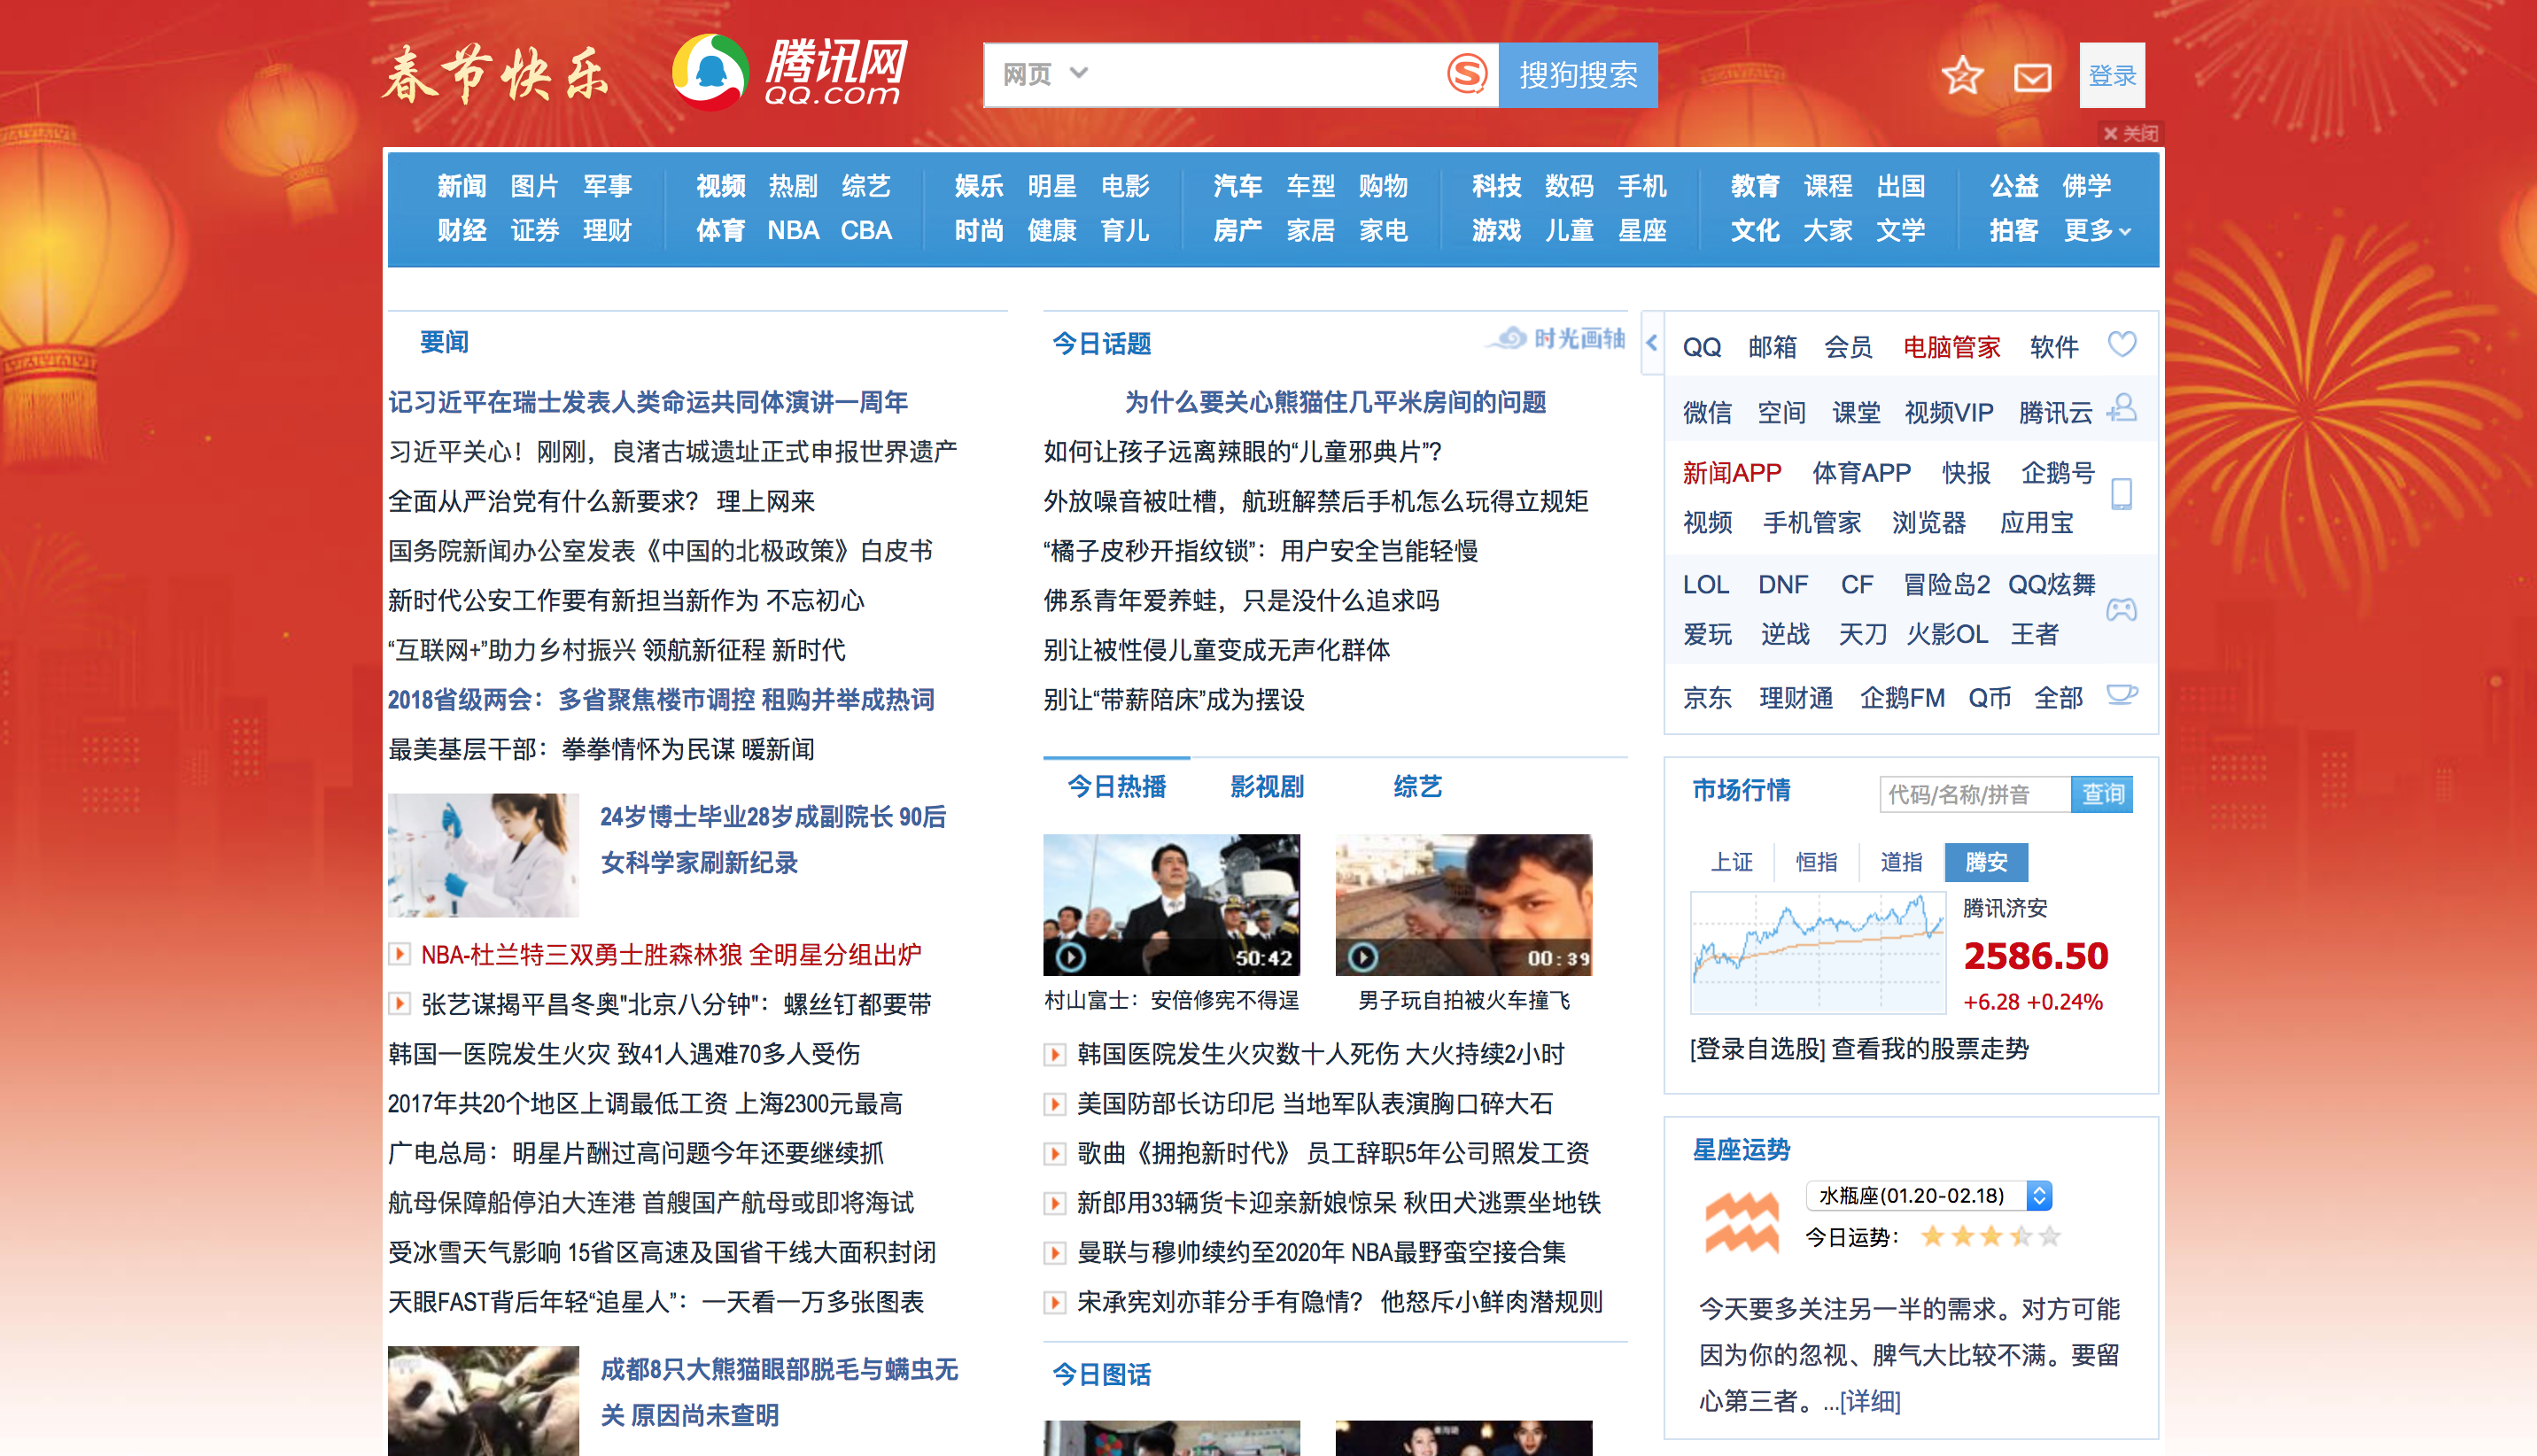
\includegraphics[width=100mm]{Images/QQ.png}
\decoRule
\caption[QQ.com]{QQ's homepage which provide which is mostly used for news.}
\label{fig:QQ.com}
\end{figure}

One element that is quite common on Chinese websites that we can see in QQ as well is it's menu bar (see fig \ref{fig:QQ_menubar}). This menu bar has two rows with a total of 40 options. This type of menu bar is quite common and can be seen at many other Chinese sites.


\begin{figure}[h]
\centering

\includegraphics[width=100mm]{Images/QQ_menubar.png}
\decoRule
\caption[QQ's Menu bar]{A close-up of the menu bar used at QQ.}
\label{fig:QQ_menubar}
\end{figure}

\subsection{BBC}

\subsection{Taobao and Ebay}
Taobao is one of the biggest websites in the world. Taobao is similar to the American Ebay in terms of what the website provide. They both are online shopping websites where you can buy almost everything you need. The design and user-experience focus on the sites are quite different. Ebay has a very sleek design with darker colors and only 20 clickable elements (see fig:\ref{fig:ebay}). Ebay also have expanding menu bar that contains about 6-10 clickable elements (see fig:\ref{fig:ebay_menu}).

\begin{figure}[h]
\centering
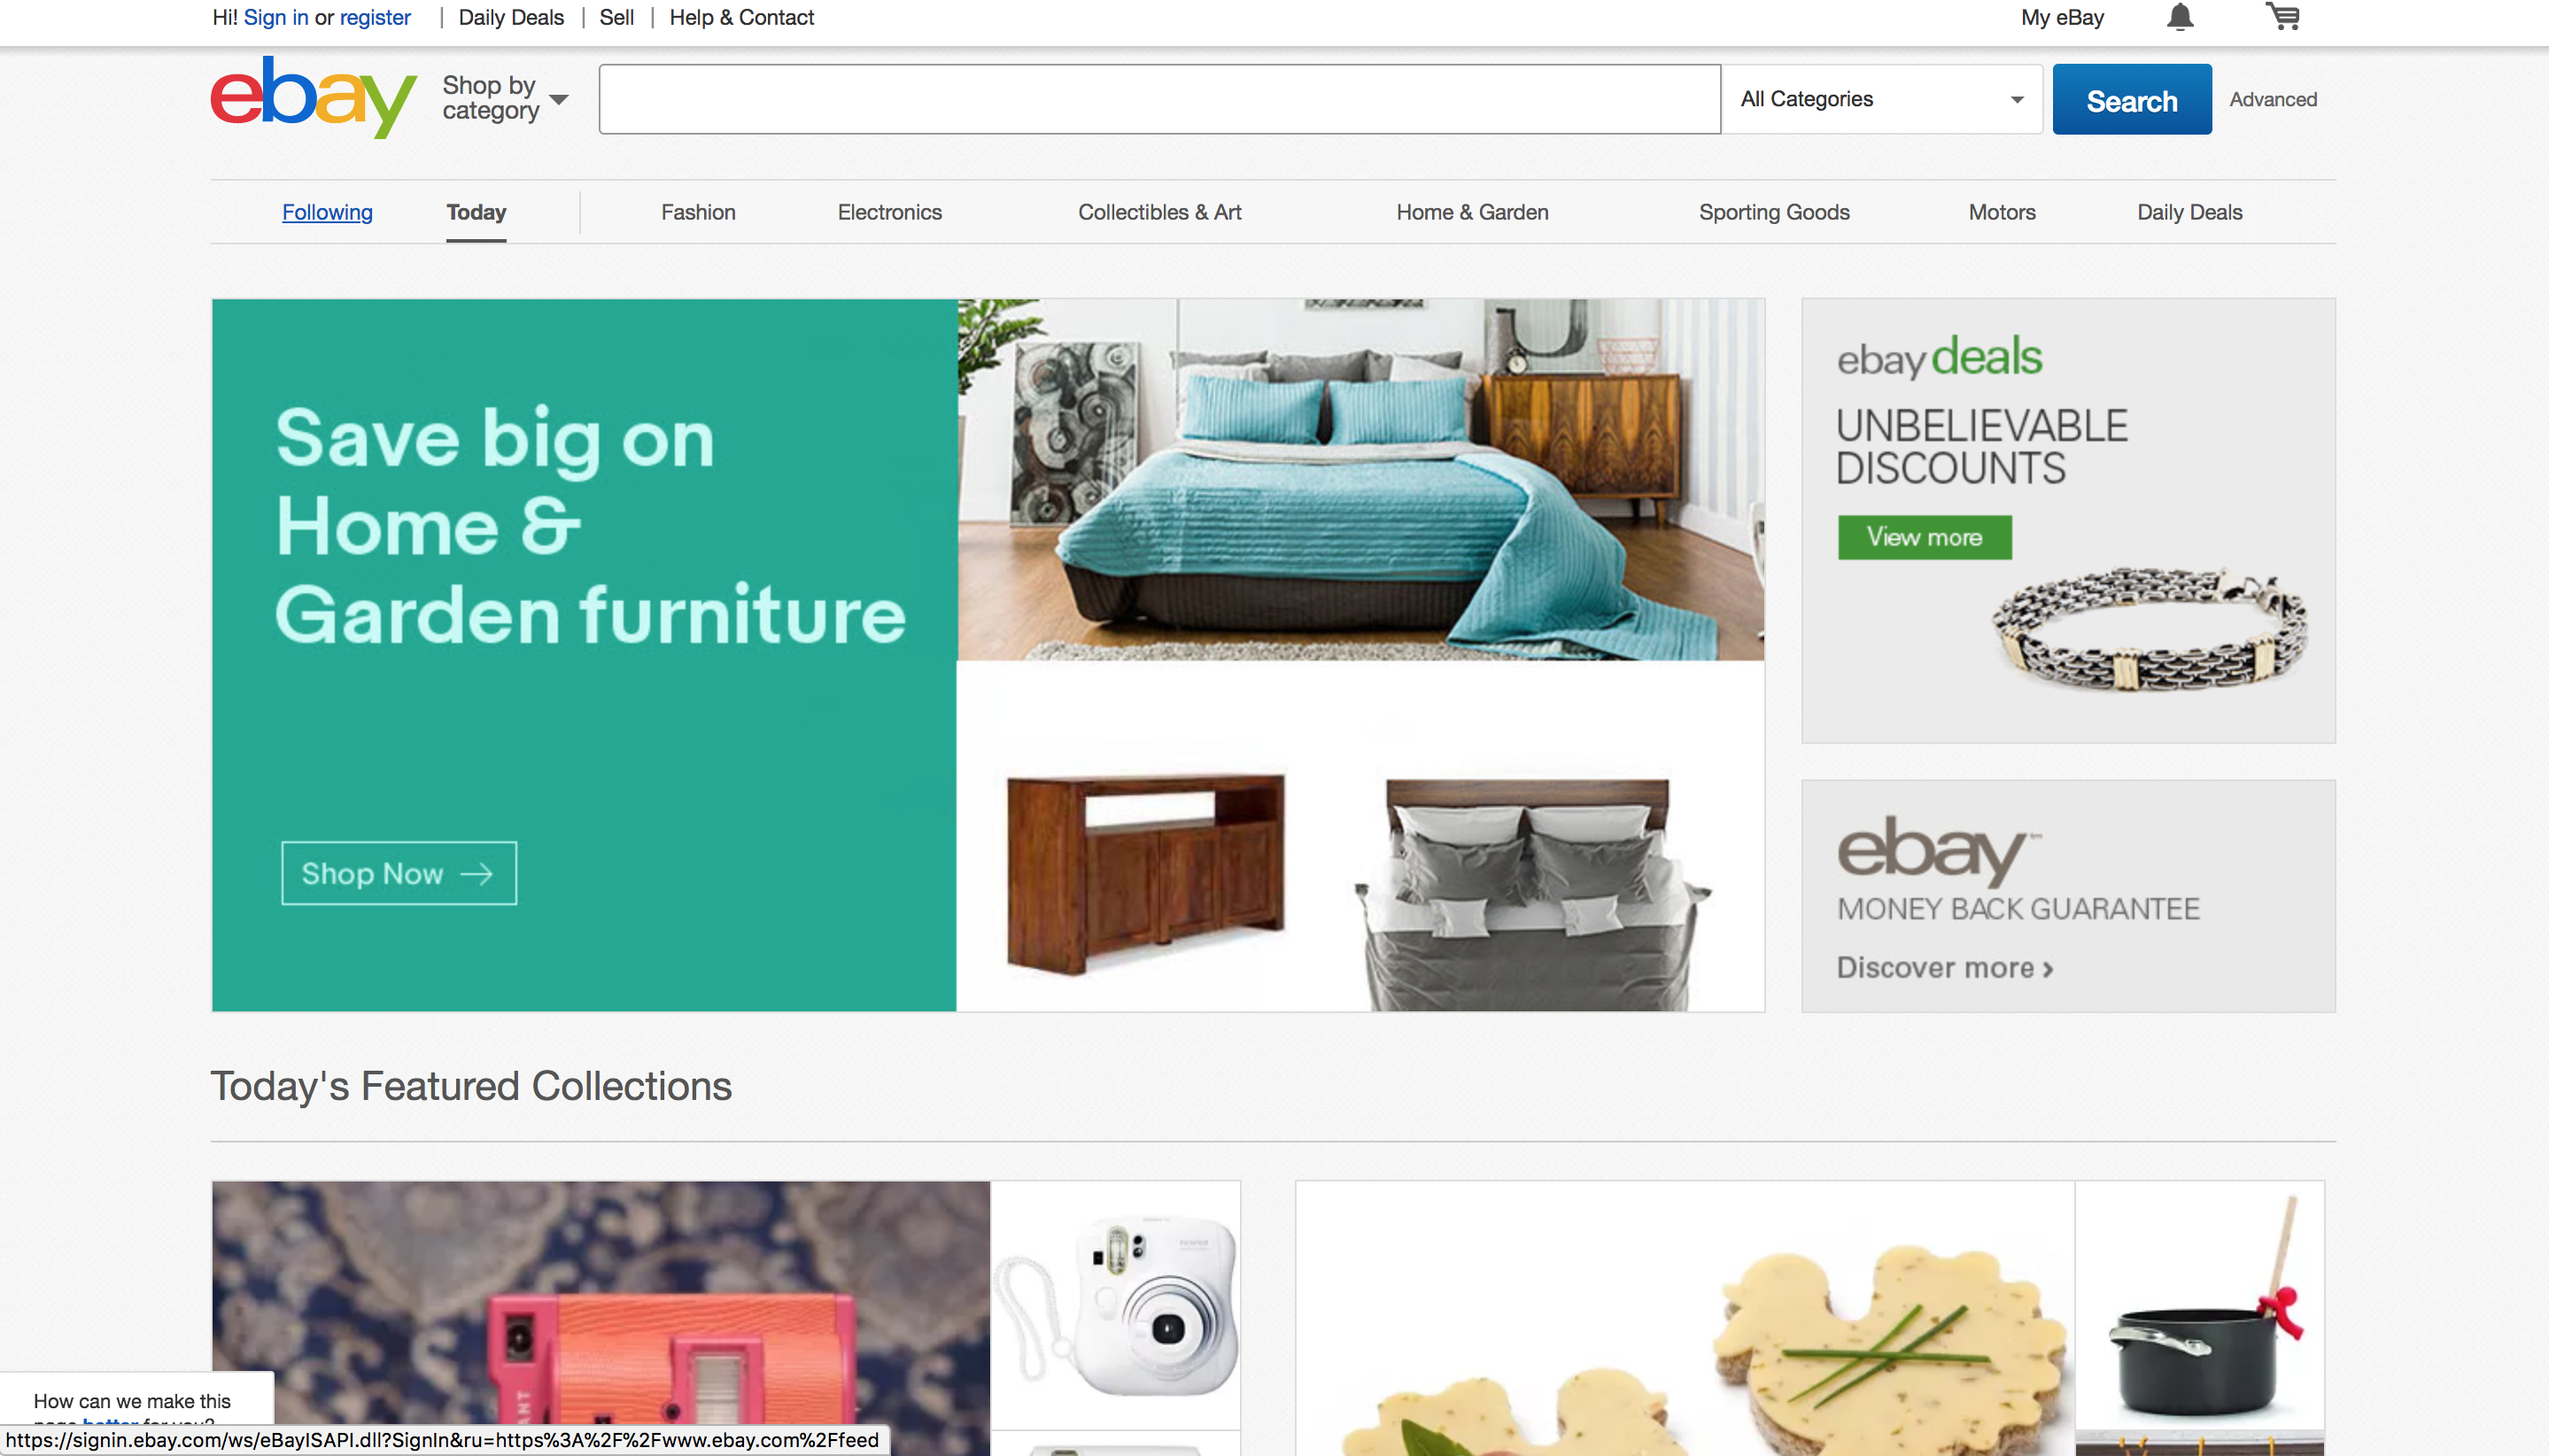
\includegraphics[width=100mm]{Images/ebay.png}
\decoRule
\caption[ebay]{Ebay a popular American online shopping site}
\label{fig:ebay}
\end{figure}

\begin{figure}[h]
\centering
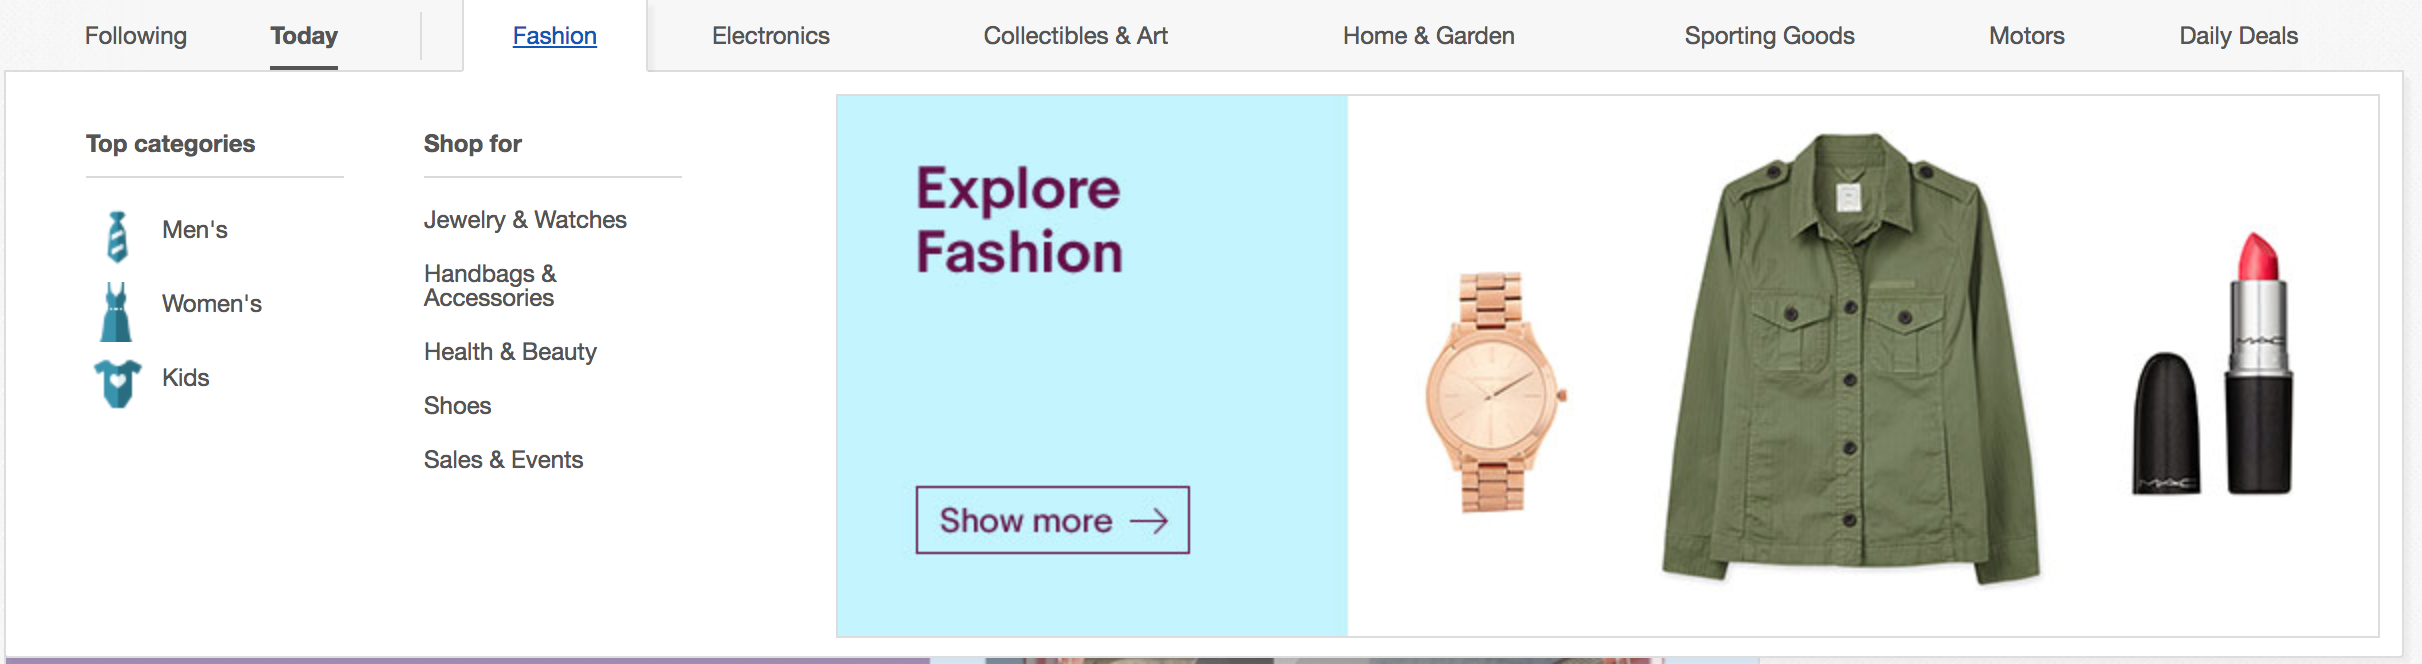
\includegraphics[width=100mm]{Images/ebay_menu.png}
\decoRule
\caption[Ebay's menu bar]{Expanding the menu on Ebay.}
\label{fig:ebay_menu}
\end{figure}

If we look at the Chinese version Taobao we once again can clearly tell the difference in information density (see fig:\ref{fig:taobao}). The main page has about 49 clickable elements. And the menu items on the right hand side can expand and show between 55-80 clickable links and elements (see fig:\ref{fig:taobao_menu}). That is about 8 times more clickable elements compared to Ebay. Another thing to take notice on Taobao is the strong colors, Taobao frequently use very strong red, purple, orange and blue. Ebay keeps more to gray and let their products provide the stronger colors to make you focus on them. 

\begin{figure}[h]
\centering
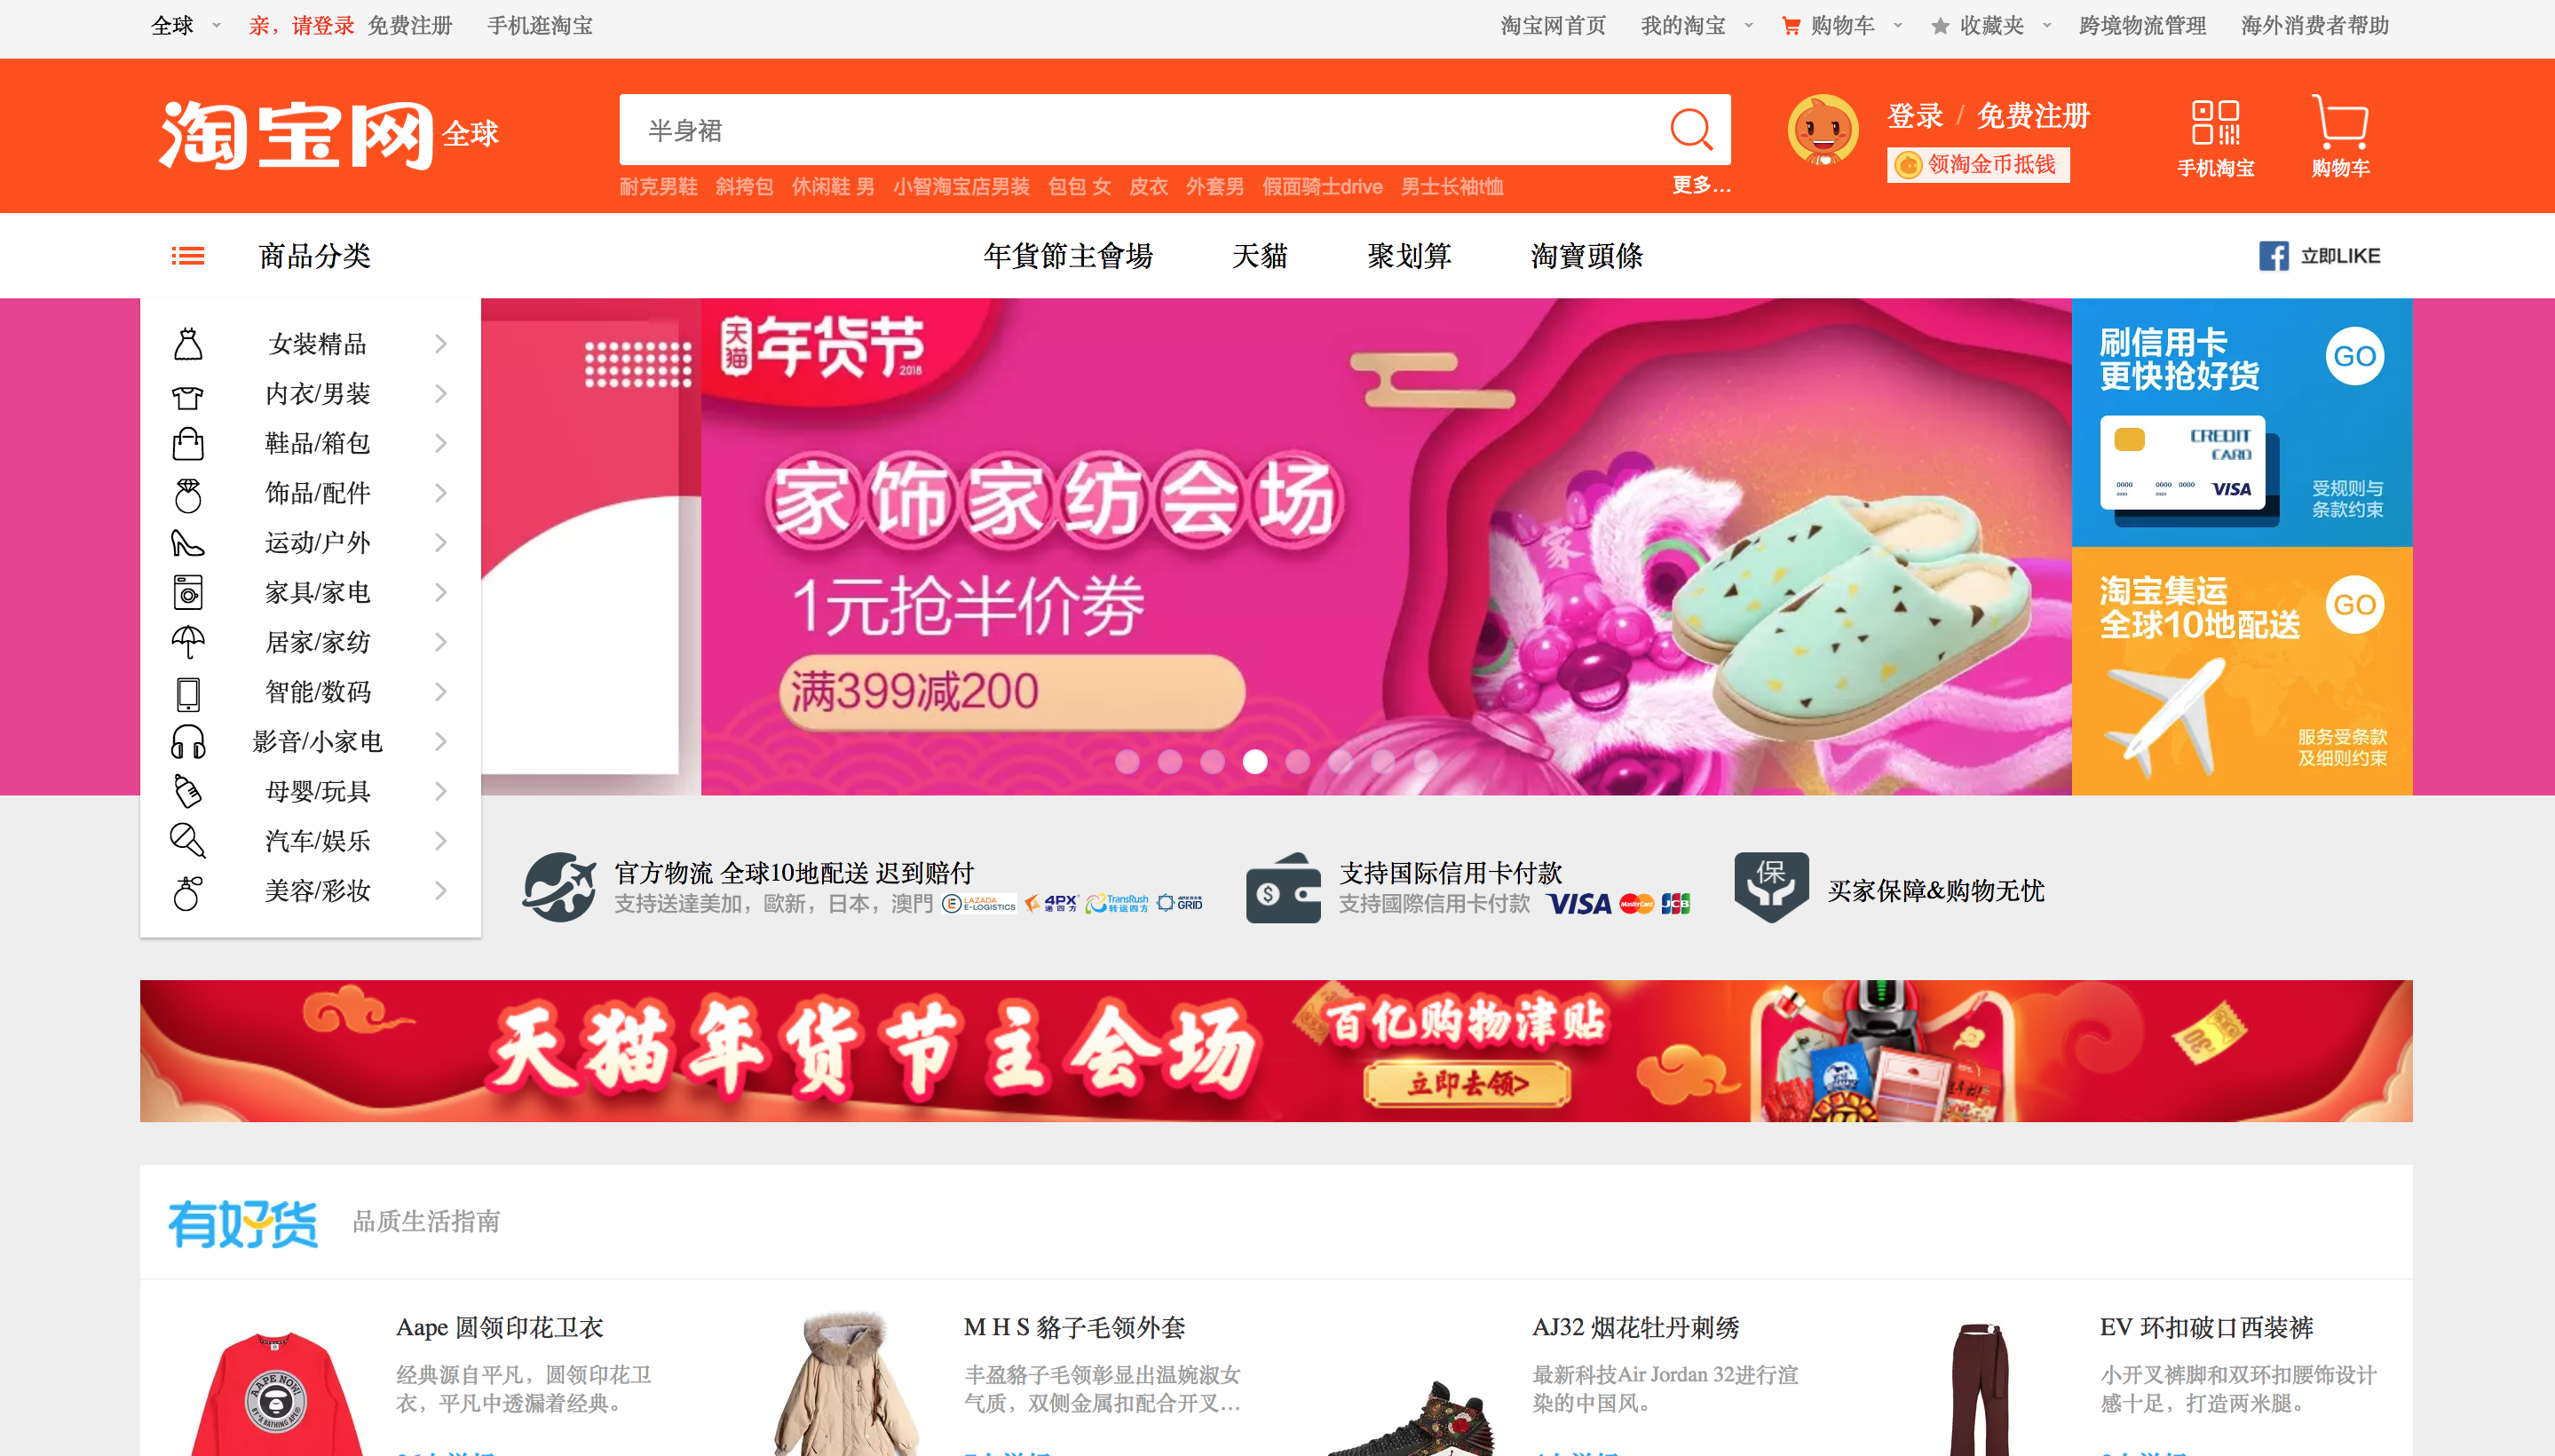
\includegraphics[width=100mm]{Images/Taobao}
\decoRule
\caption[Taobao]{Taobao a popular Chinese online shopping site}
\label{fig:taobao}
\end{figure}

\begin{figure}[h]
\centering
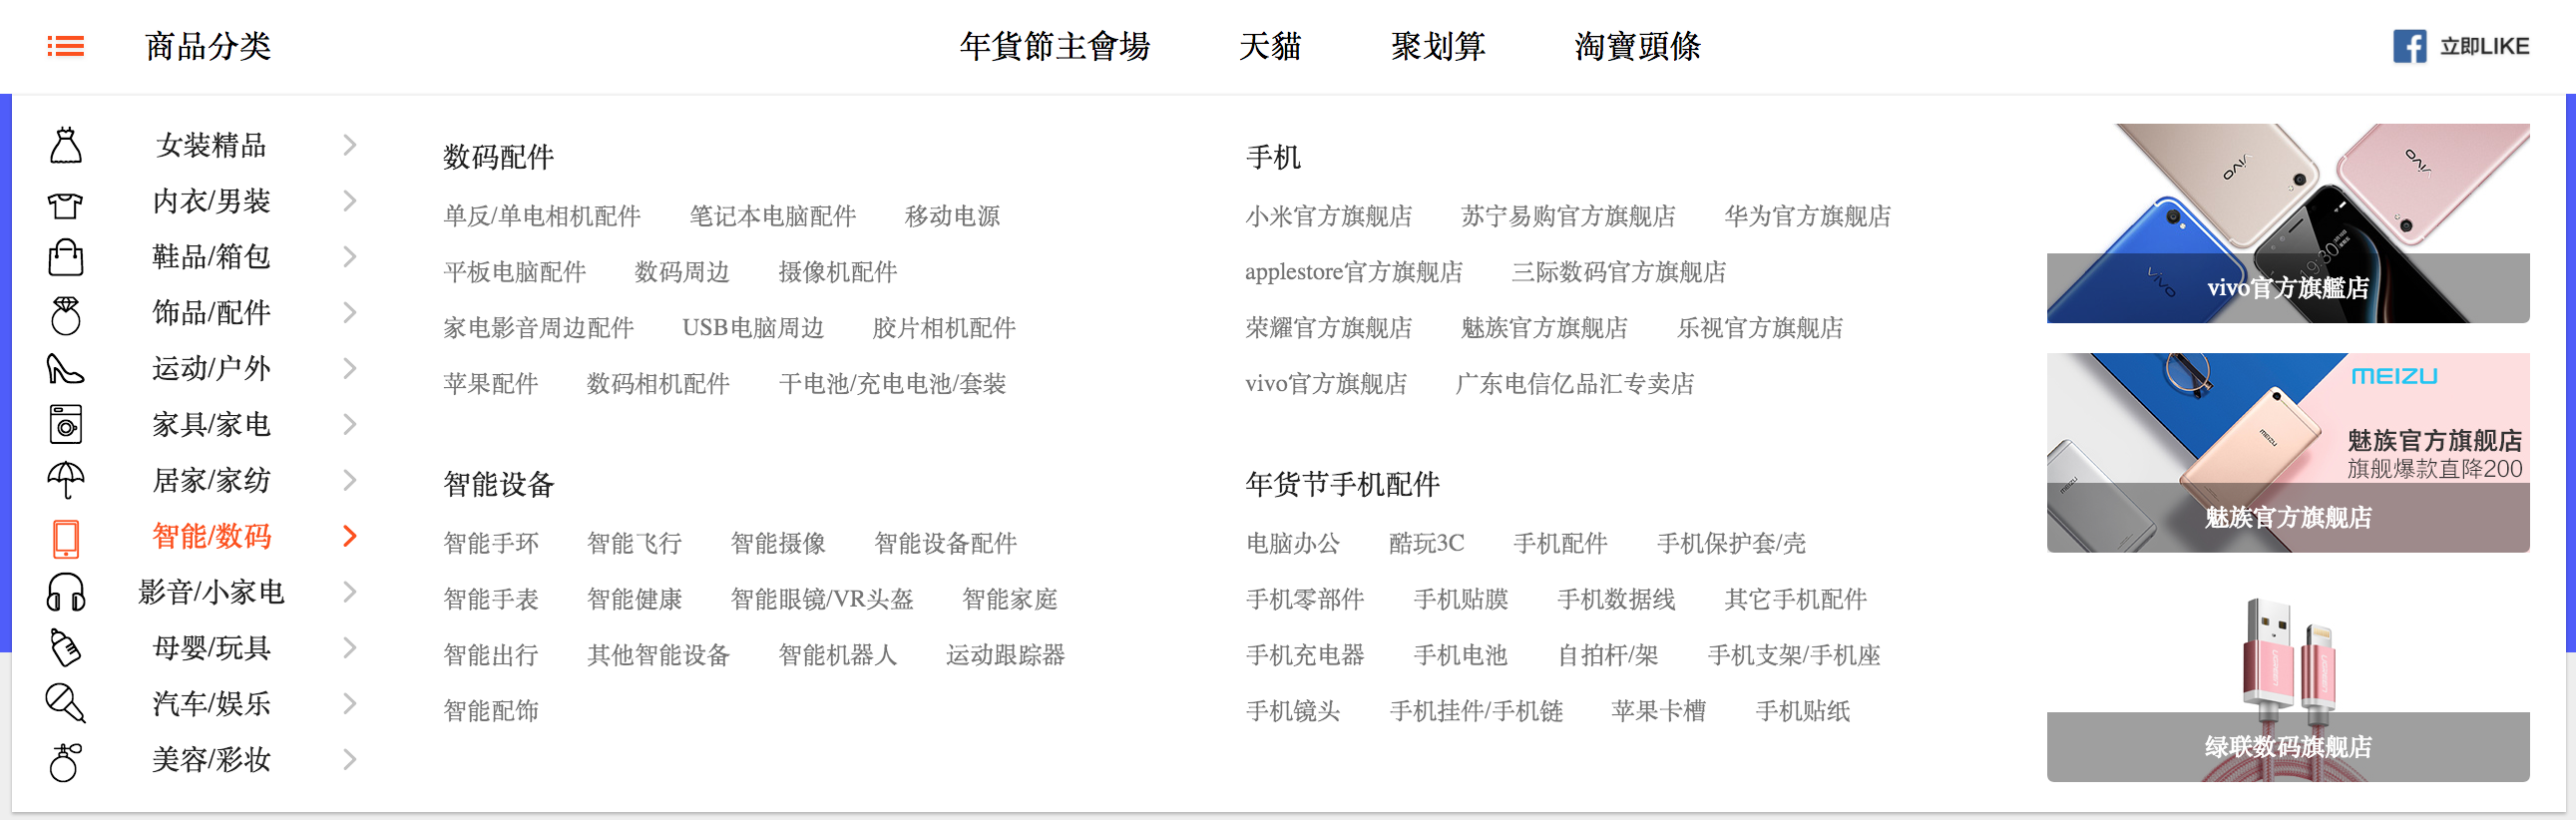
\includegraphics[width=100mm]{Images/Taobao_menu}
\decoRule
\caption[Taobao' menu bar]{Expanding the menu on Taobao.}
\label{fig:taobao_menu}
\end{figure}

\subsection{Analyses of Ctrip}
Many Chinese web sites change quite a lot when changing language. Ctrip is one of these sites. Ctrip is a very common travel site in China which allows you to book hotels, flights, car rental etc. When you select to translate this site to English it does not only translate the site but the whole layout and design of the website change as well (see  fig: \ref{fig:ctrip_chinese} for Chinese version and fig: \ref{fig:ctrip_english} for English version). Except for the brand and name of the website you can barely tell that it is the same site.

\begin{figure}[h]
\centering
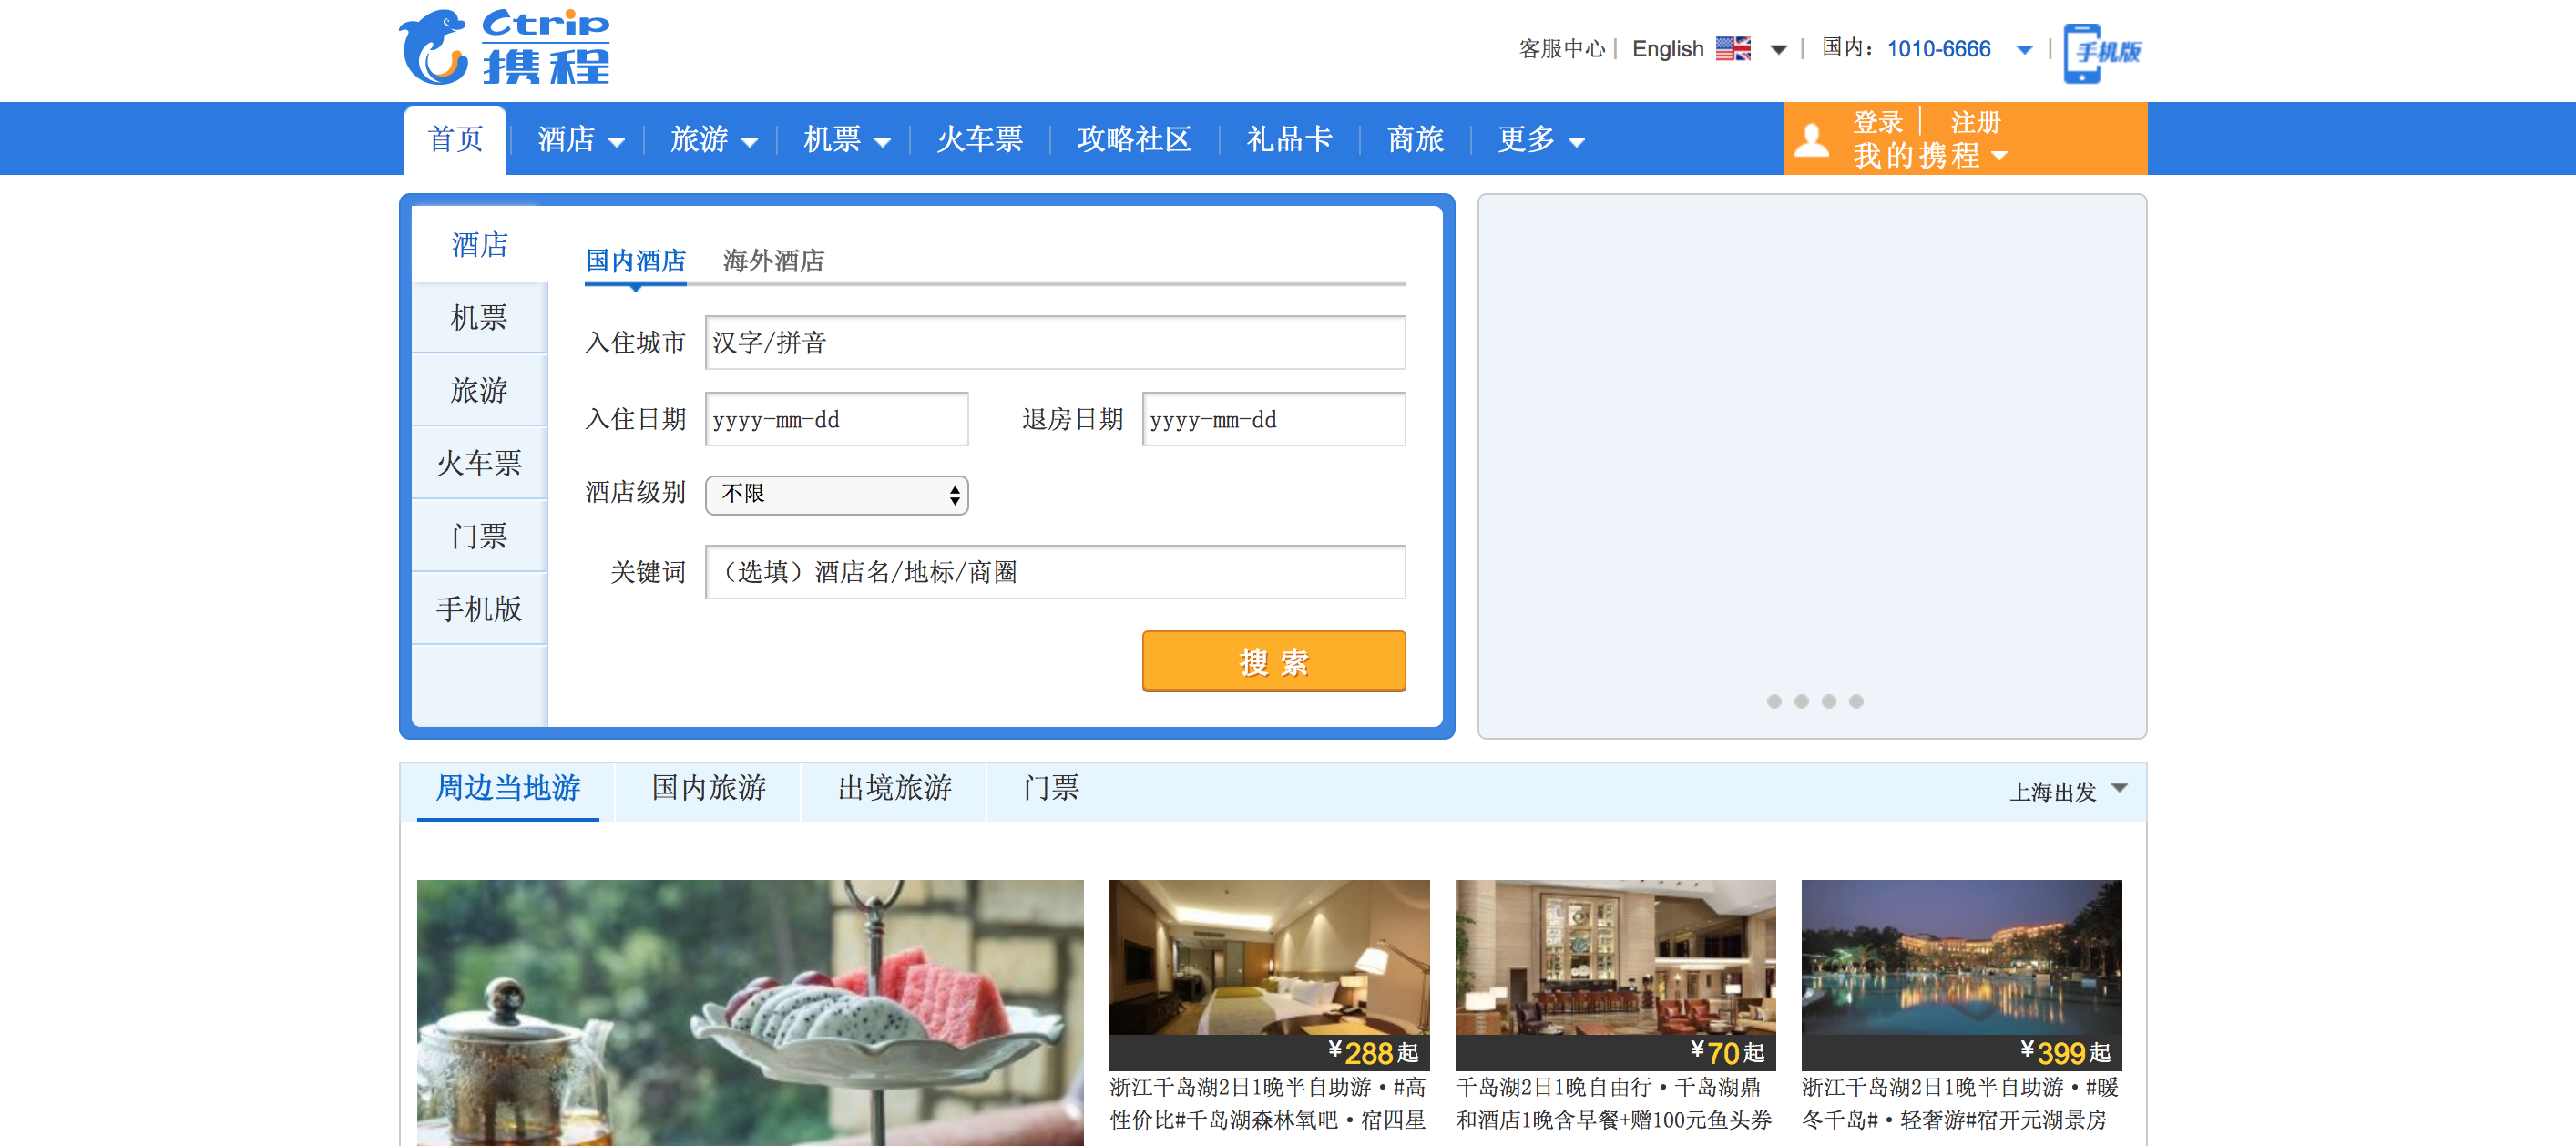
\includegraphics[width=100mm]{Images/ctrip_chinese1}
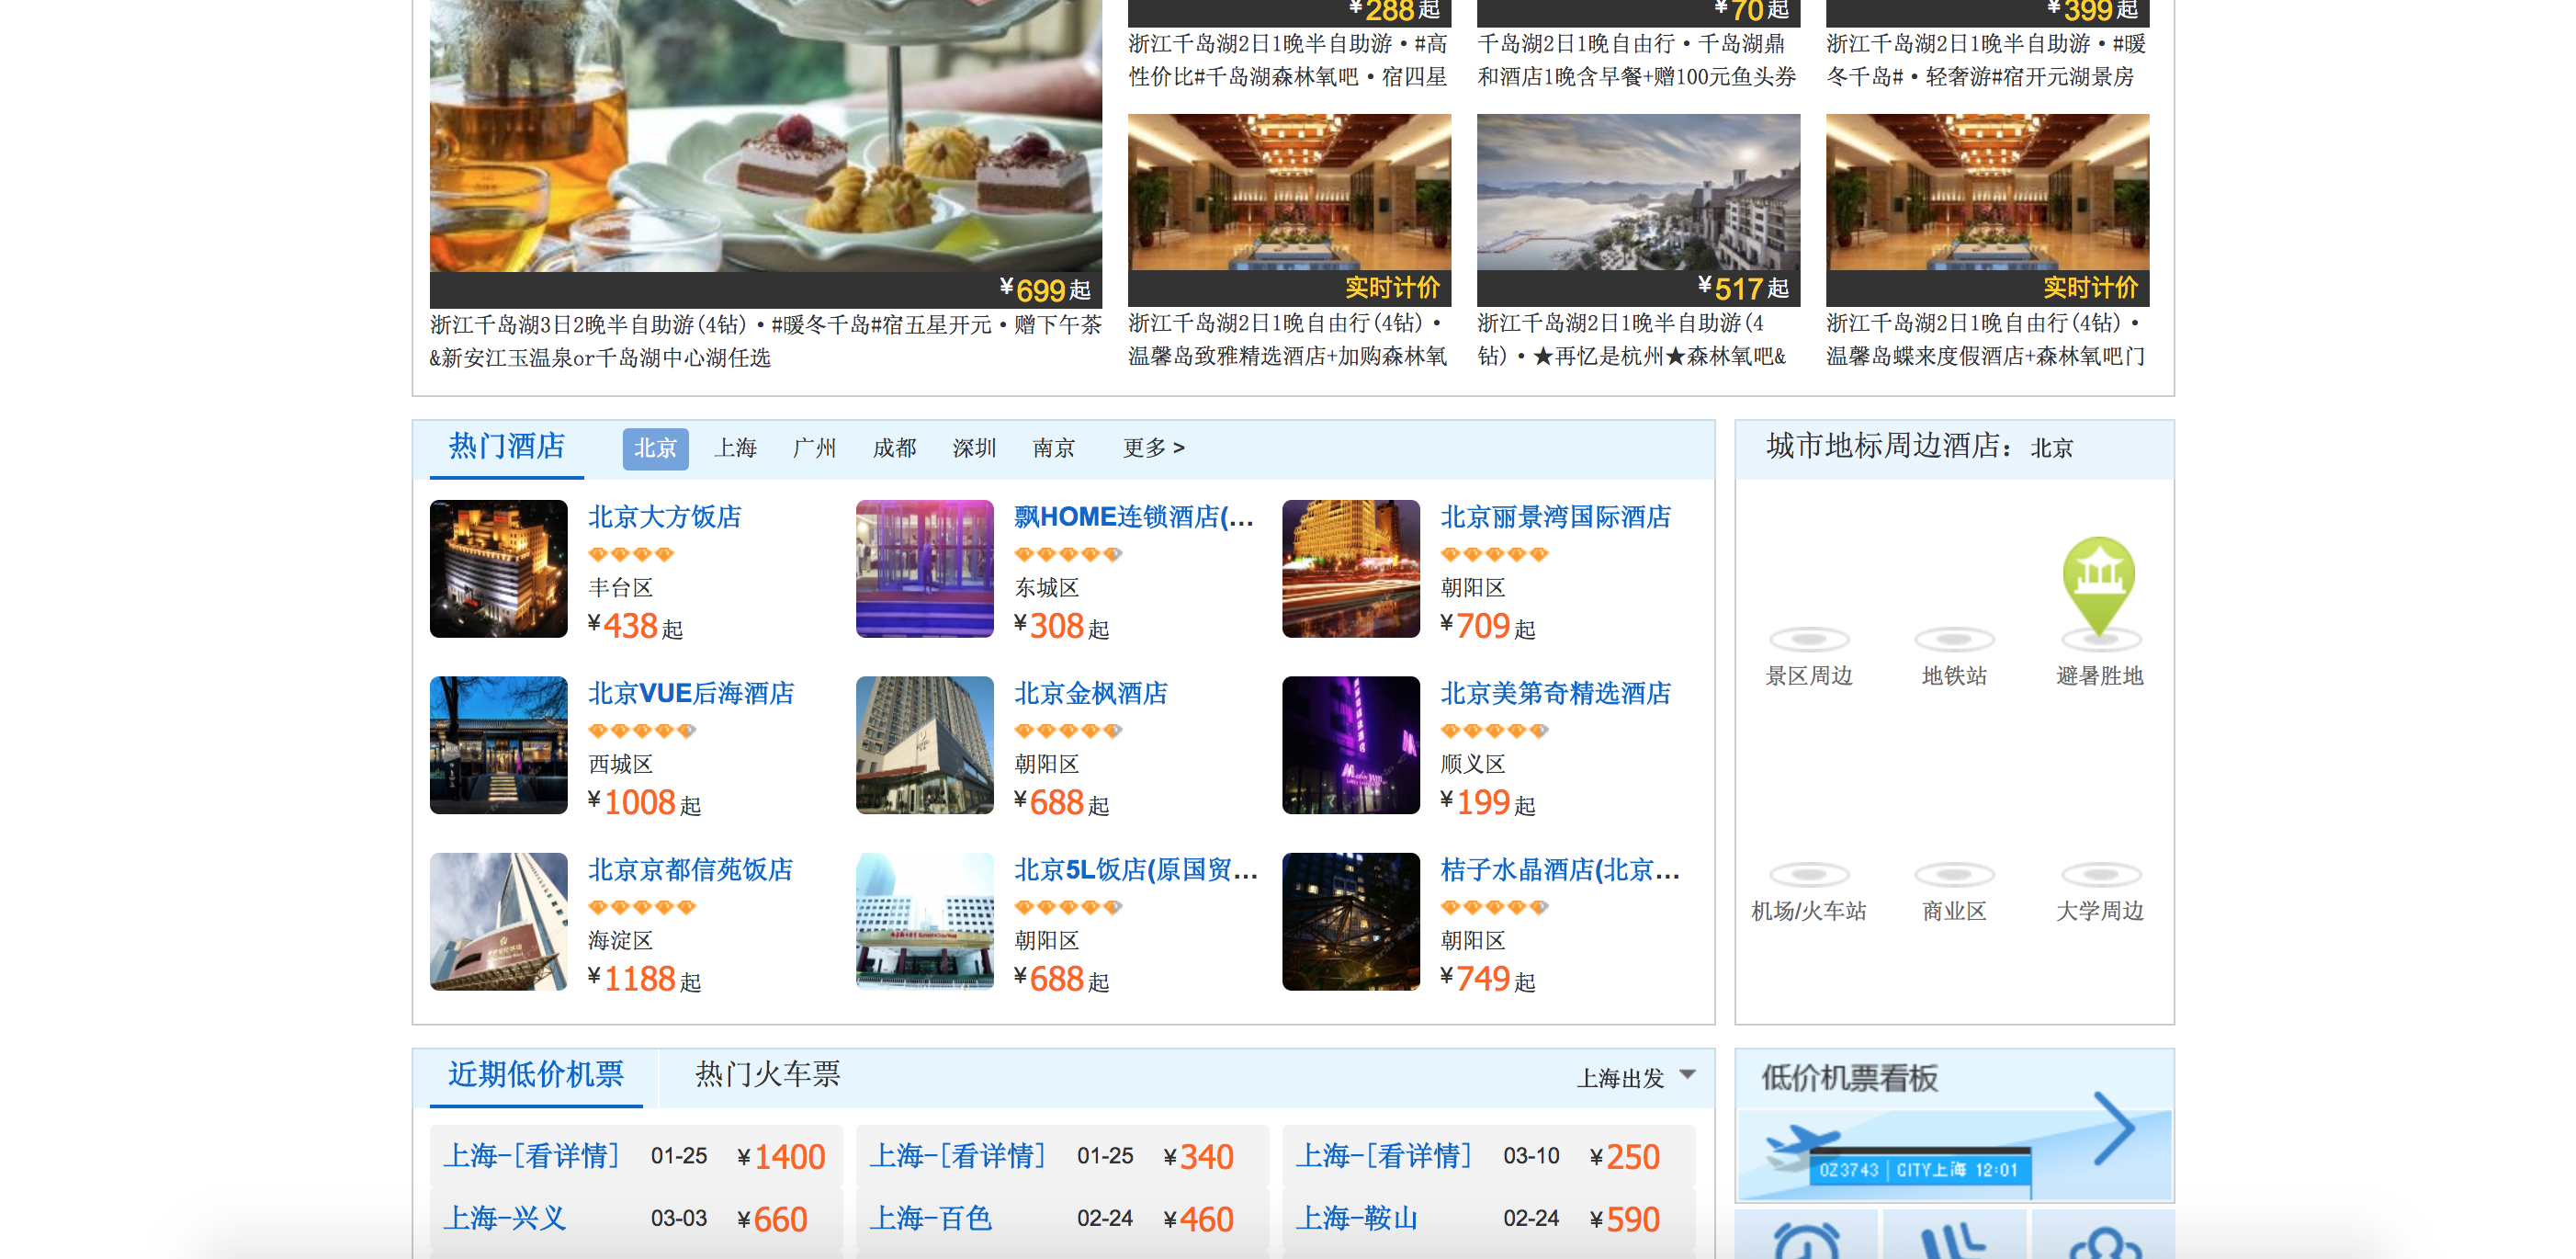
\includegraphics[width=100mm]{Images/ctrip_chinese2}
\decoRule
\caption[Chinese version of Ctrip]{The Chinese version of the travel website Ctrip.}
\label{fig:ctrip_chinese}
\end{figure}

\begin{figure}[h]
\centering
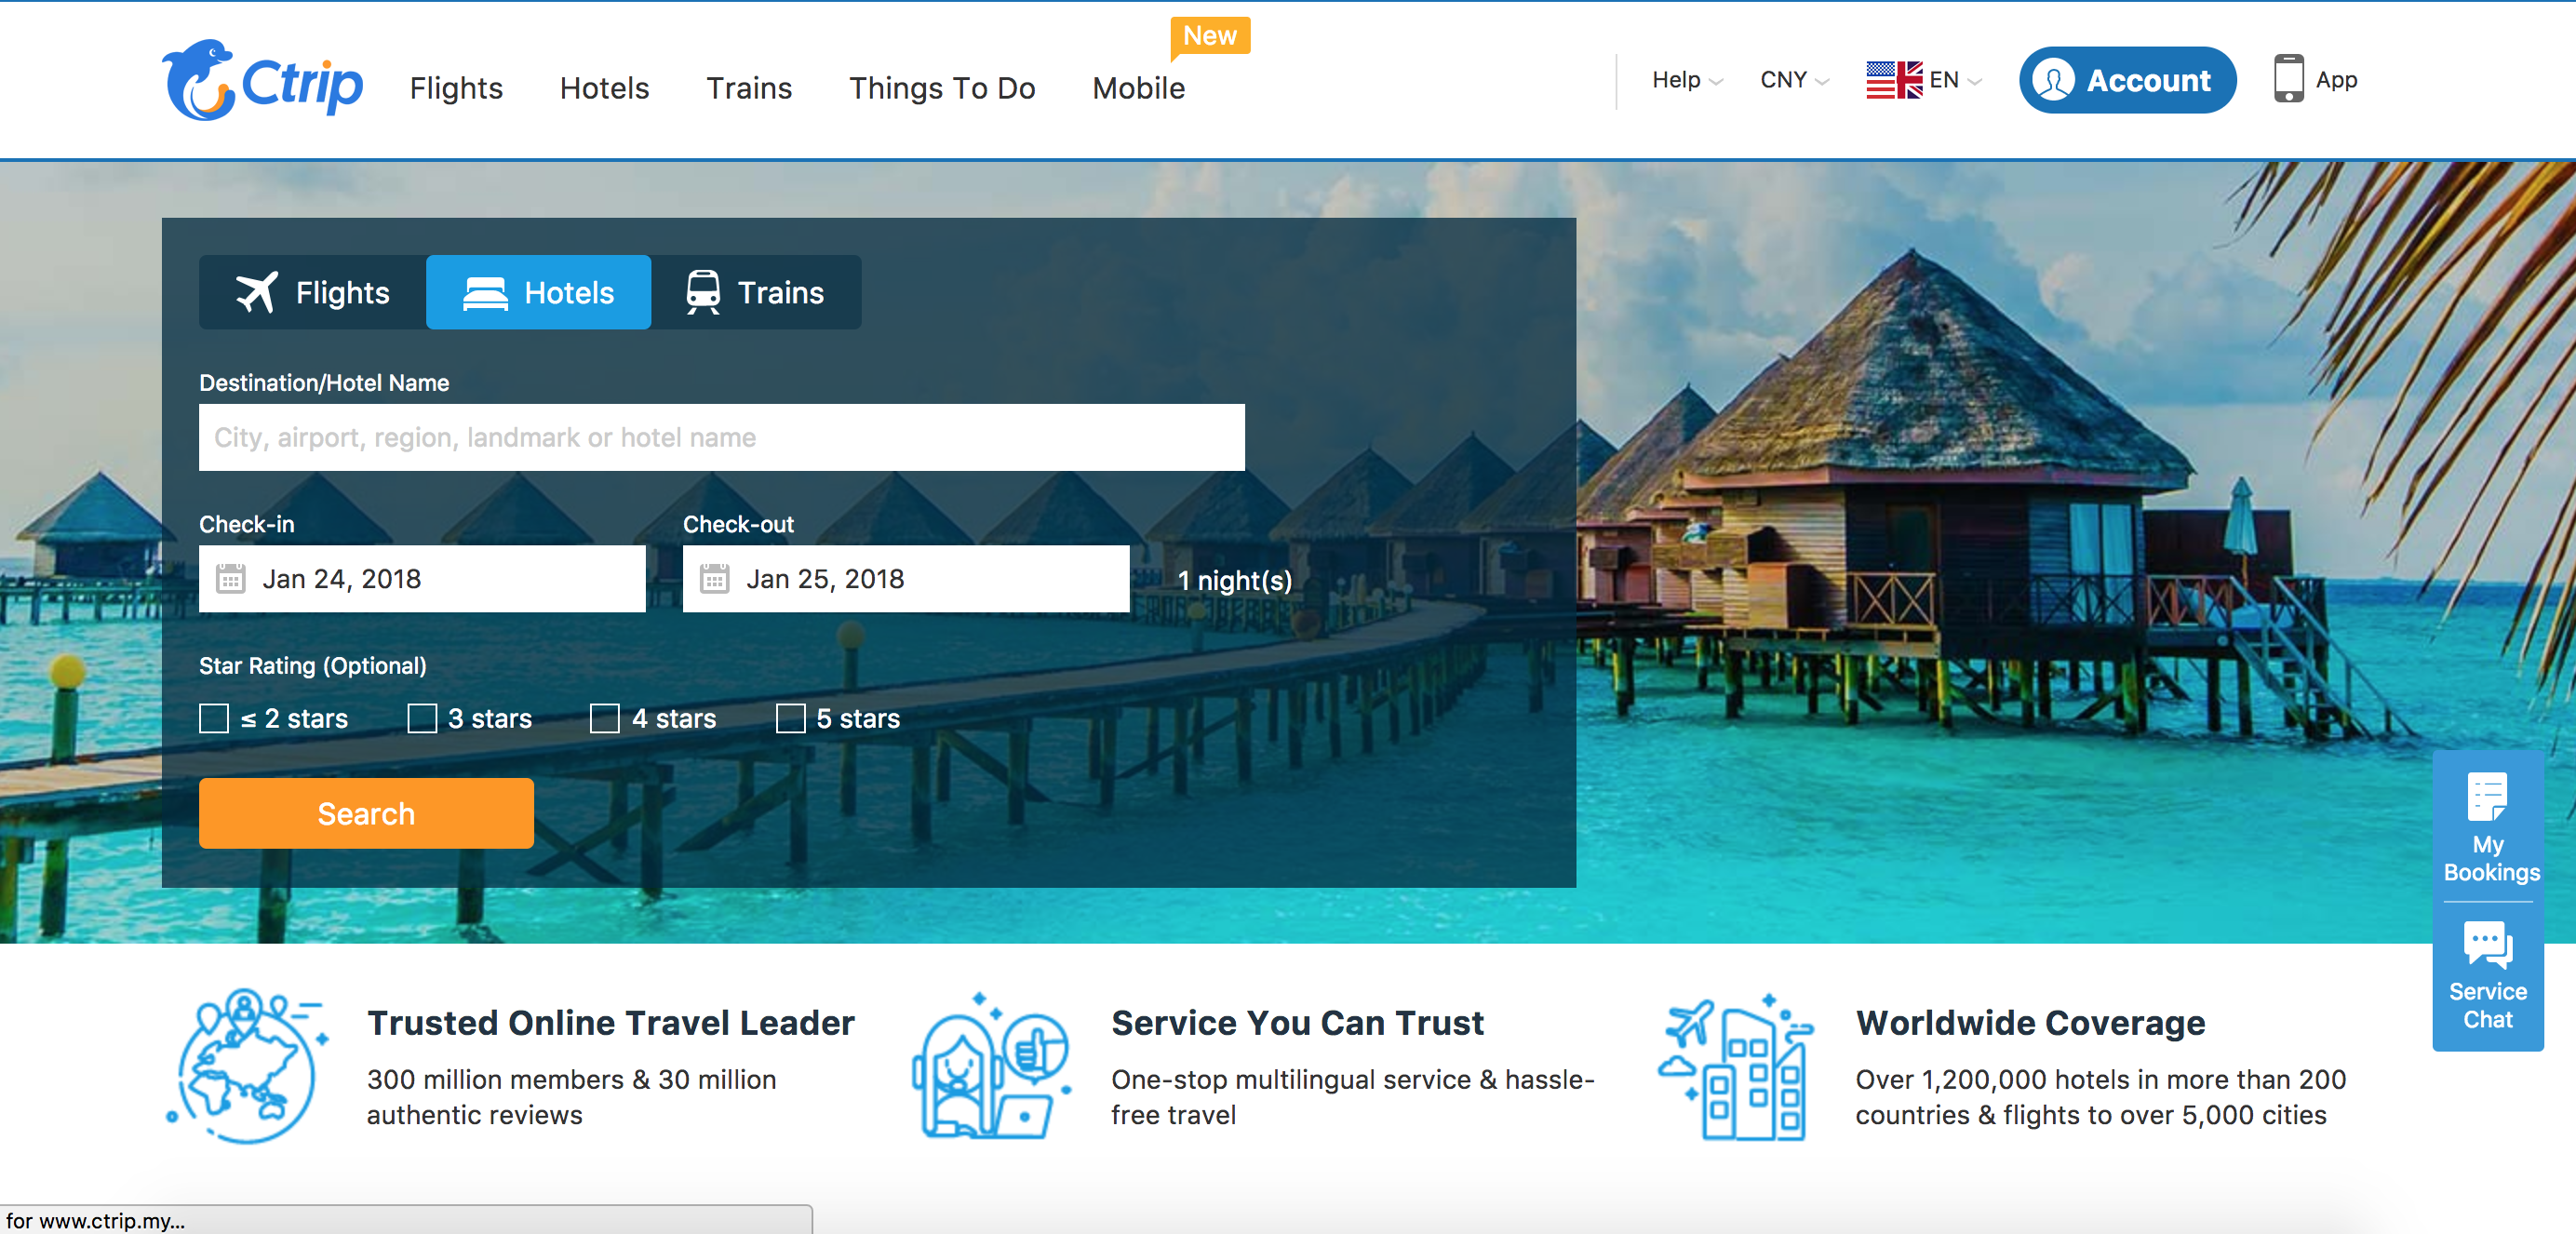
\includegraphics[width=100mm]{Images/ctrip_eng1}
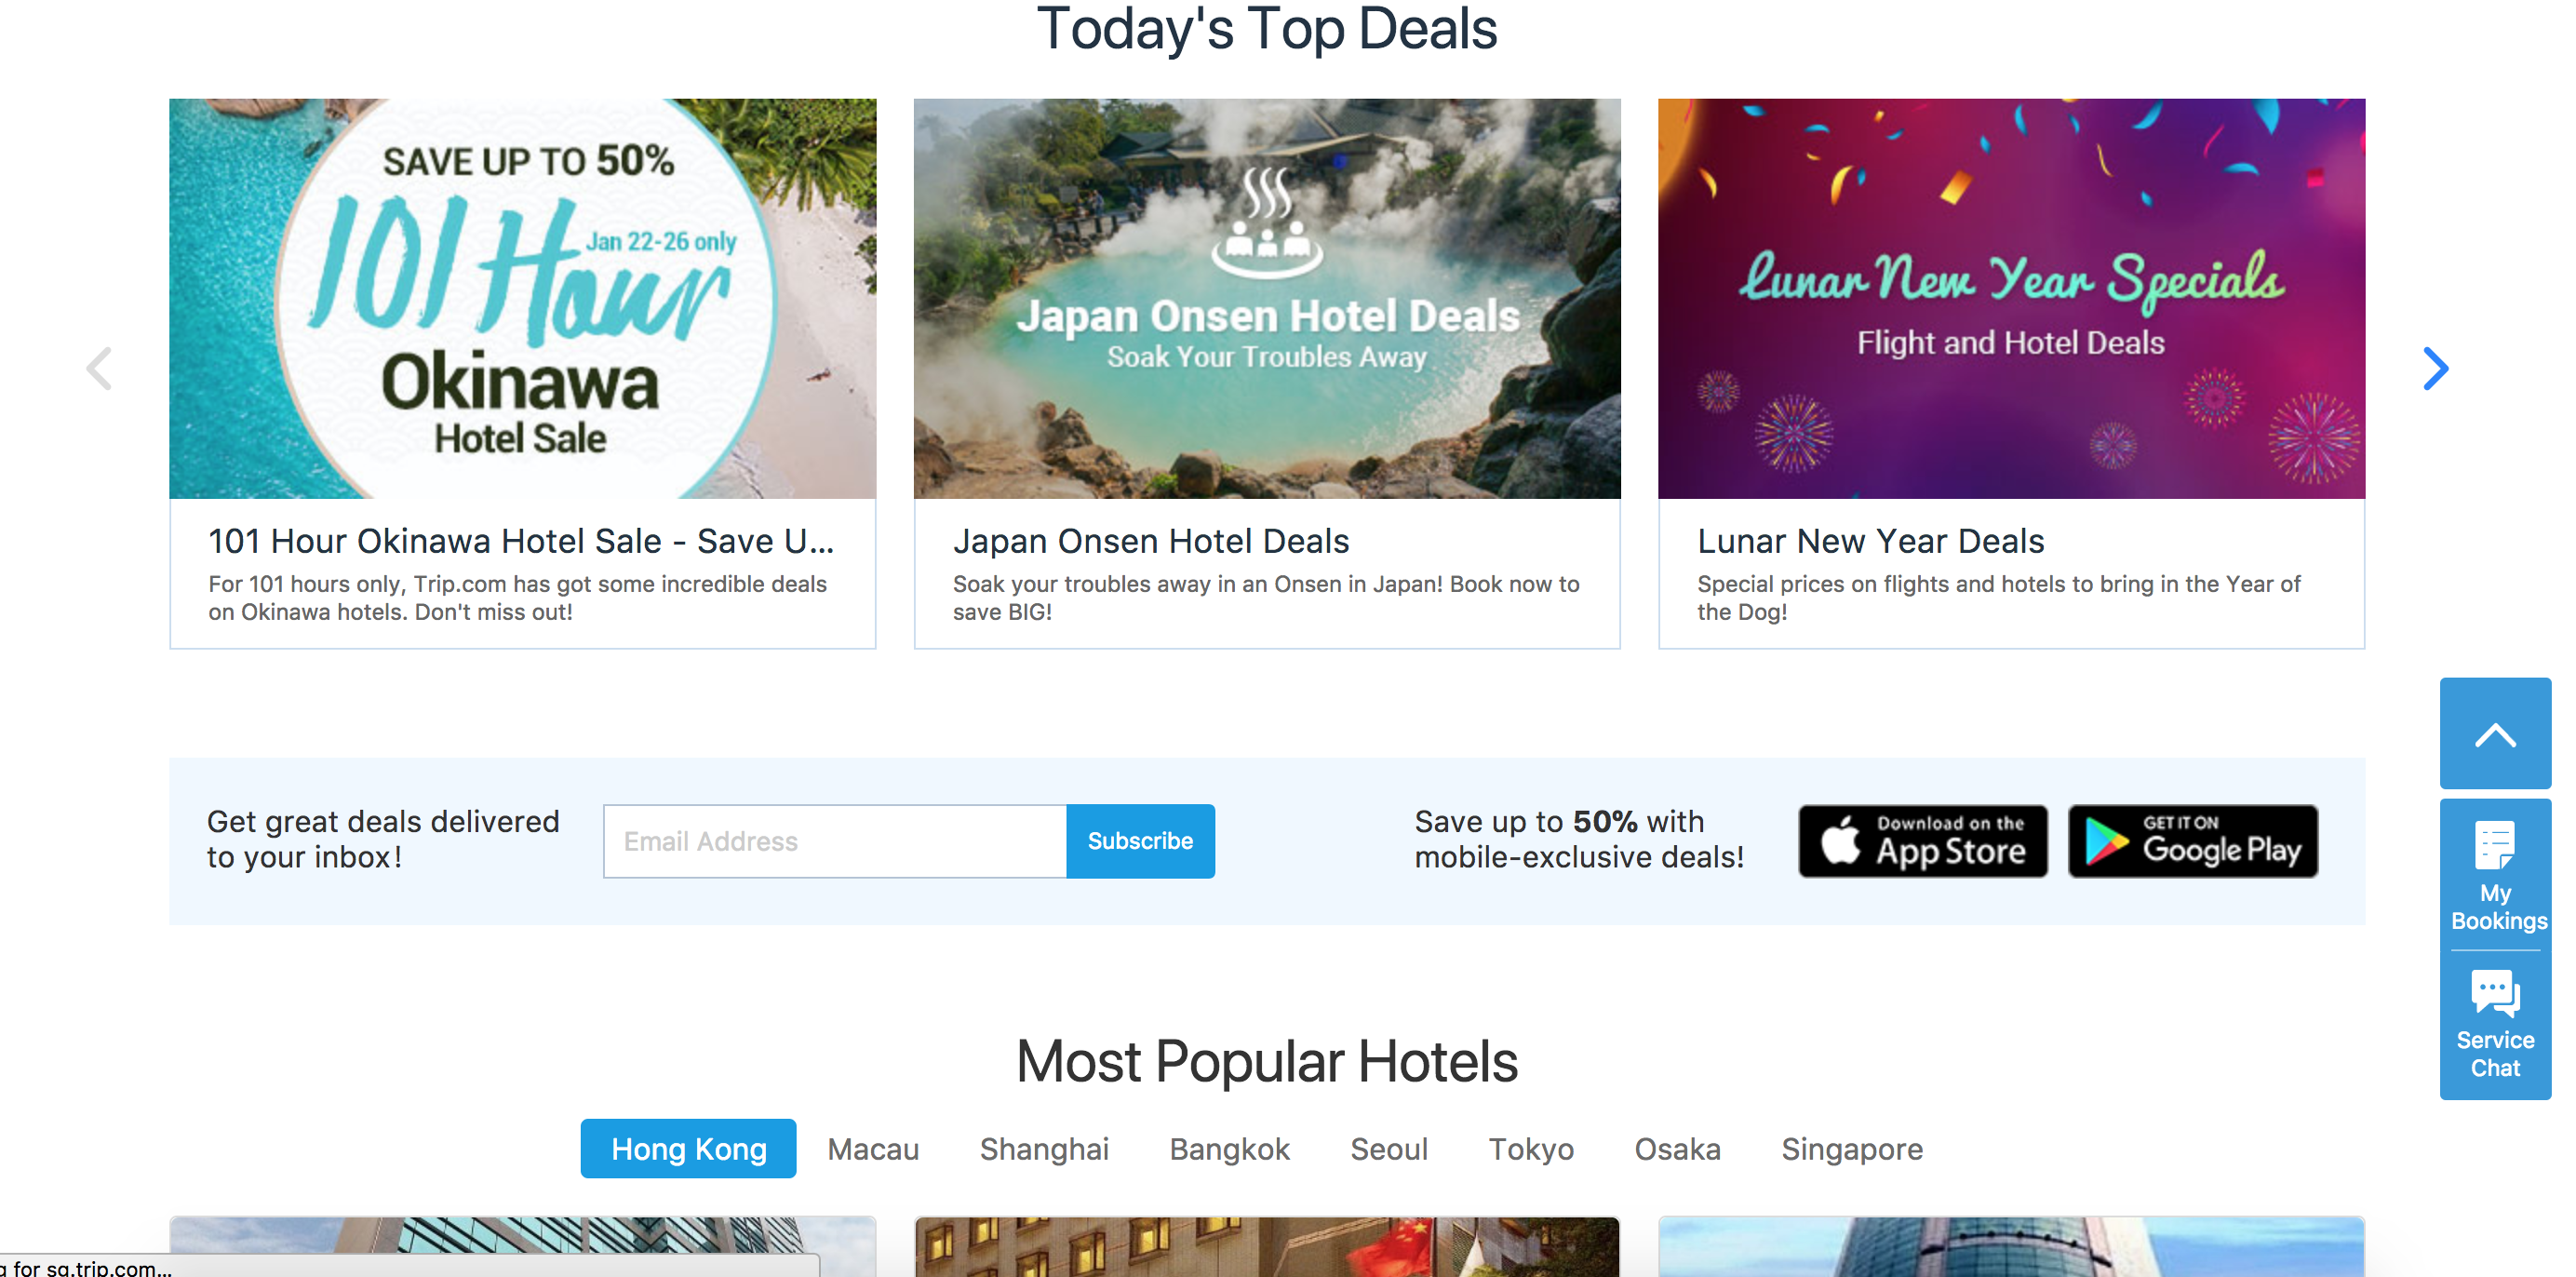
\includegraphics[width=100mm]{Images/ctrip_eng2}
\decoRule
\caption[English version of Ctrip]{The English version of the travel website Ctrip.}
\label{fig:ctrip_english}
\end{figure}
 The main difference we can see between these sites is the density of content. The Chinese version has a lot more content on a smaller area. Counting clickable elements without hovering over anything we can find 40 clickable elements on the Chinese version compared to 26 clickable elements on the English version. When using the Chinese site all links open a separate window instead of a second menu or tab. This is a quite common phenomena found in many sites.
 
 
 
\newpage
 \section{Conclusion Phase 1}
 \subsection{Common Chinese design that differs from western design}
Looking through the websites we can identify several design features (outside of the language differences) that differ in Chinese and western websites. 
\\\\
These are:
 \begin{itemize}
 \item High information density
 \item Colors
 \item Ad content
 \item Navigation
 \end{itemize}
 
 The main factor we could see across all websites is the difference in information density. Chinese websites have significantly higher information density compared to their western counterparts. This is one feature we want to examine more closely in our later study. Colors and navigation will be explored but not prioritized. These will be included to give a more accurate feel of the site instead of focused on. Chinese sites have a higher ad content than many of the western counterparts, this is a feature that not will be looked into in this study.   There are several hypothesis for why Chinese sites are so information dense. Some of these hypothesis are: cultural/trends, historical, holistic vs analytic perceptions (ref or cite..) and language. Because of limitations with understanding of the Chinese language, history and culture we will mainly examine trends and perception.
 \\\\
  To do this we will create two interfaces, one western inspired and one with inspiration from Chinese designs. To make sure that the interfaces will look Chinese and Western we will with the help from professional UX-designers from Sweden and China develop some prototypes. The prototypes will then be tested on both users with Swedish and Chinese heritage respectively. We will later develop a working interface from these prototypes that will be able to measure what the users do in response to certain tasks. Main measurements that will be used are task-success, time-on-task and a modified System usability scale. \cite{brooke1996sus} 
  \\\\
  Four interfaces will be created, with two following a western design and the other two using a Chinese layout. The first interface takes inspiration from the QQ and BBC news site home pages. The goal of implementing these interfaces is to explore how fluidly users from different cultural backgrounds can navigate sites containing high information density (e.g., copious amounts of images and texts ). Both interfaces contain roughly equivalent levels of material and clickable elements; the primary difference is that the western site will be longer, forcing users to scroll down the page. Additionally, some of the information will be mapped in sub-menus using natural mapping for the western site \cite{Norman}. Conversely, the Chinese inspired site will provide most of the material directly on the screen for users to view without any nested menus. 
  \\\\
  Categorization of Data
  \\\\
  Choosing the ux questions:
  In \cite{Holistic_vs_Analytic} has shown that perception differs in western and eastern cultures. \cite{cross_web} further proves that this is true in the case of people observing websites where users with analytic perception follows the F-shaped pattern \cite{pernice2014people}. Holistic people on the other hand does not follow the F-shaped pattern when browsing through a website. \cite{cross_web} One Interesting aspect to look into is how this affect performance when looking for specific elements. To do this we will select elements both in accordance to the F-shaped pattern and elements outside of this pattern. By testing the performance on both analytical and holistic minded people we should hopefully get a indication if there is any difference and how well people follow the F-shaped pattern when looking for a specific element. The test will be unsupervised which means that we will have to get a larger test audience to get any significant results. To test this we will create test for the sites BBC and QQ where we will ask the test subject to find elements inside the F-shaped pattern range and also outside
  F-shaped pattern vs non F-shaped (\cite{cross_web})
  Information density
   
 \subsection{Limitations}
 Even if many of the biggest websites in china are quite information dense there are several websites that have adopted a sleeker look for their sites/services. Two big examples of this is the messenger application WeChat which is very big in china and the the Alipay service website. I will not focus on sites like this and there might be a trend in china that is moving towards a sleeker look. In this report i have specifically chosen the some of the most popular regularly used sites that differ from the western design standard. In the case of Taobao it might seem very difficult for many westerners to use but it is as of now one of the biggest websites in the world. There are also cases of websites more or less copying western websites because they are blocked in China. A typical example of this is youku and youtube, these types of sites will not be focused on in this report either.
 
 \section{Lägg till}
 Undersök lite angående functionalitet samt vilka du kan lägga till i sidan 
% Chapter Template

\chapter{Phase 2 - Prototyping} % Main chapter title

\label{Chapter5} % Change X to a consecutive number; for referencing this chapter elsewhere, use \ref{ChapterX}

%----------------------------------------------------------------------------------------
%	SECTION 1
%----------------------------------------------------------------------------------------
The goal of Phase 2 is to quickly create prototypes for our design that achieve what we want for the project. The prototypes will then be tested so that the actual website will have some testing behind it before building and thereby enable a quicker development.

\section{Method}


\section{Results}
\subsubsection{Low-fi Prototype}

\subsubsection{High-fi Prototype}

\section{Conclusion Phase 2}



\subsection{Limitations} 
% Chapter Template

\chapter{Phase 3 - Building the Interfaces} % Main chapter title

\label{Chapter6} % Change X to a consecutive number; for referencing this chapter elsewhere, use \ref{ChapterX}

%----------------------------------------------------------------------------------------
%	SECTION 1
%----------------------------------------------------------------------------------------
The goal for this phase is to develop the beta-test,test it, update according to feedback and deploy it. After the web test has been deployed it will be accessible. Several different technologies will be used and described in this chapter to make all of this possible.
\section{Method}
To be able to perform the test on users all over the world without actually having to be there a web based test had to be constructed. The test was made using several different technologies and hosted on aws. 

Several things had to be taken into consideration such as: slower network in china, possibility of web connection getting interrupted, measuring correct behaviours, making sure a completable devices was used for the test (mobile device would not at all test the same thing).


\subsection{Front-End}
The most important front-end technology on this website are React, Redux and Redux-Sagas. These three libraries create most of the functionality in website and they work very closely together. With React we show the user what we want him or her to see. All the users behaviours are stored in Redux (imagine a database for the browser), then depending on the updates in Redux, React appropriately up dates the information the users see. Some of the actions a user does triggers a Saga (Example: Pressing the finish button). That Saga then makes a asynchronous call to our API and send over the data stored in Redux to our mysql database hosted on AWS in Seoul. 
\\\\
Our front-end consist of four different pages. Homepage, bbc, qq, sus and done. The names of these pages are taken from the material that inspired them. The bbc site is not a actual bbc site but is named so since it is inspired from the bbc website. These namings is not something the users see and therefore does not affect them it's only to make it clear what page that is currently being disused. The flow of the test is as follows: The user starts at the Homepage, depending on the last test made by someone the user will either end up at the bbc page or the qq page. Depending on the language selected by this user they will see the page in the selected language. After finishing the bbc or qq test the user will be taken to the questionnaire on the sus page. After this is completed the user will arrive at the done page which contain a simple message thanking the user for their participation and provide my contact information if they have any questions. 

\subsubsection{Homepage}
The homepage is the first page the user will see. This page is responsible for gathering information needed to decide how the rest of the test will be set-up. The homepage will start by asking the user if they want to do the test in Chinese or English. The test will then proceed to give the user information about the test in their chosen language. The web page will then query the database to check which of the sites that have the least number of tests done (bbc or qq). The user will then be see a description of the test in the selected language (see \ref{fig:homepage} ). After the user finishes reading the description and press "start" the site will start the test.

\begin{figure}[h]
	\centering
	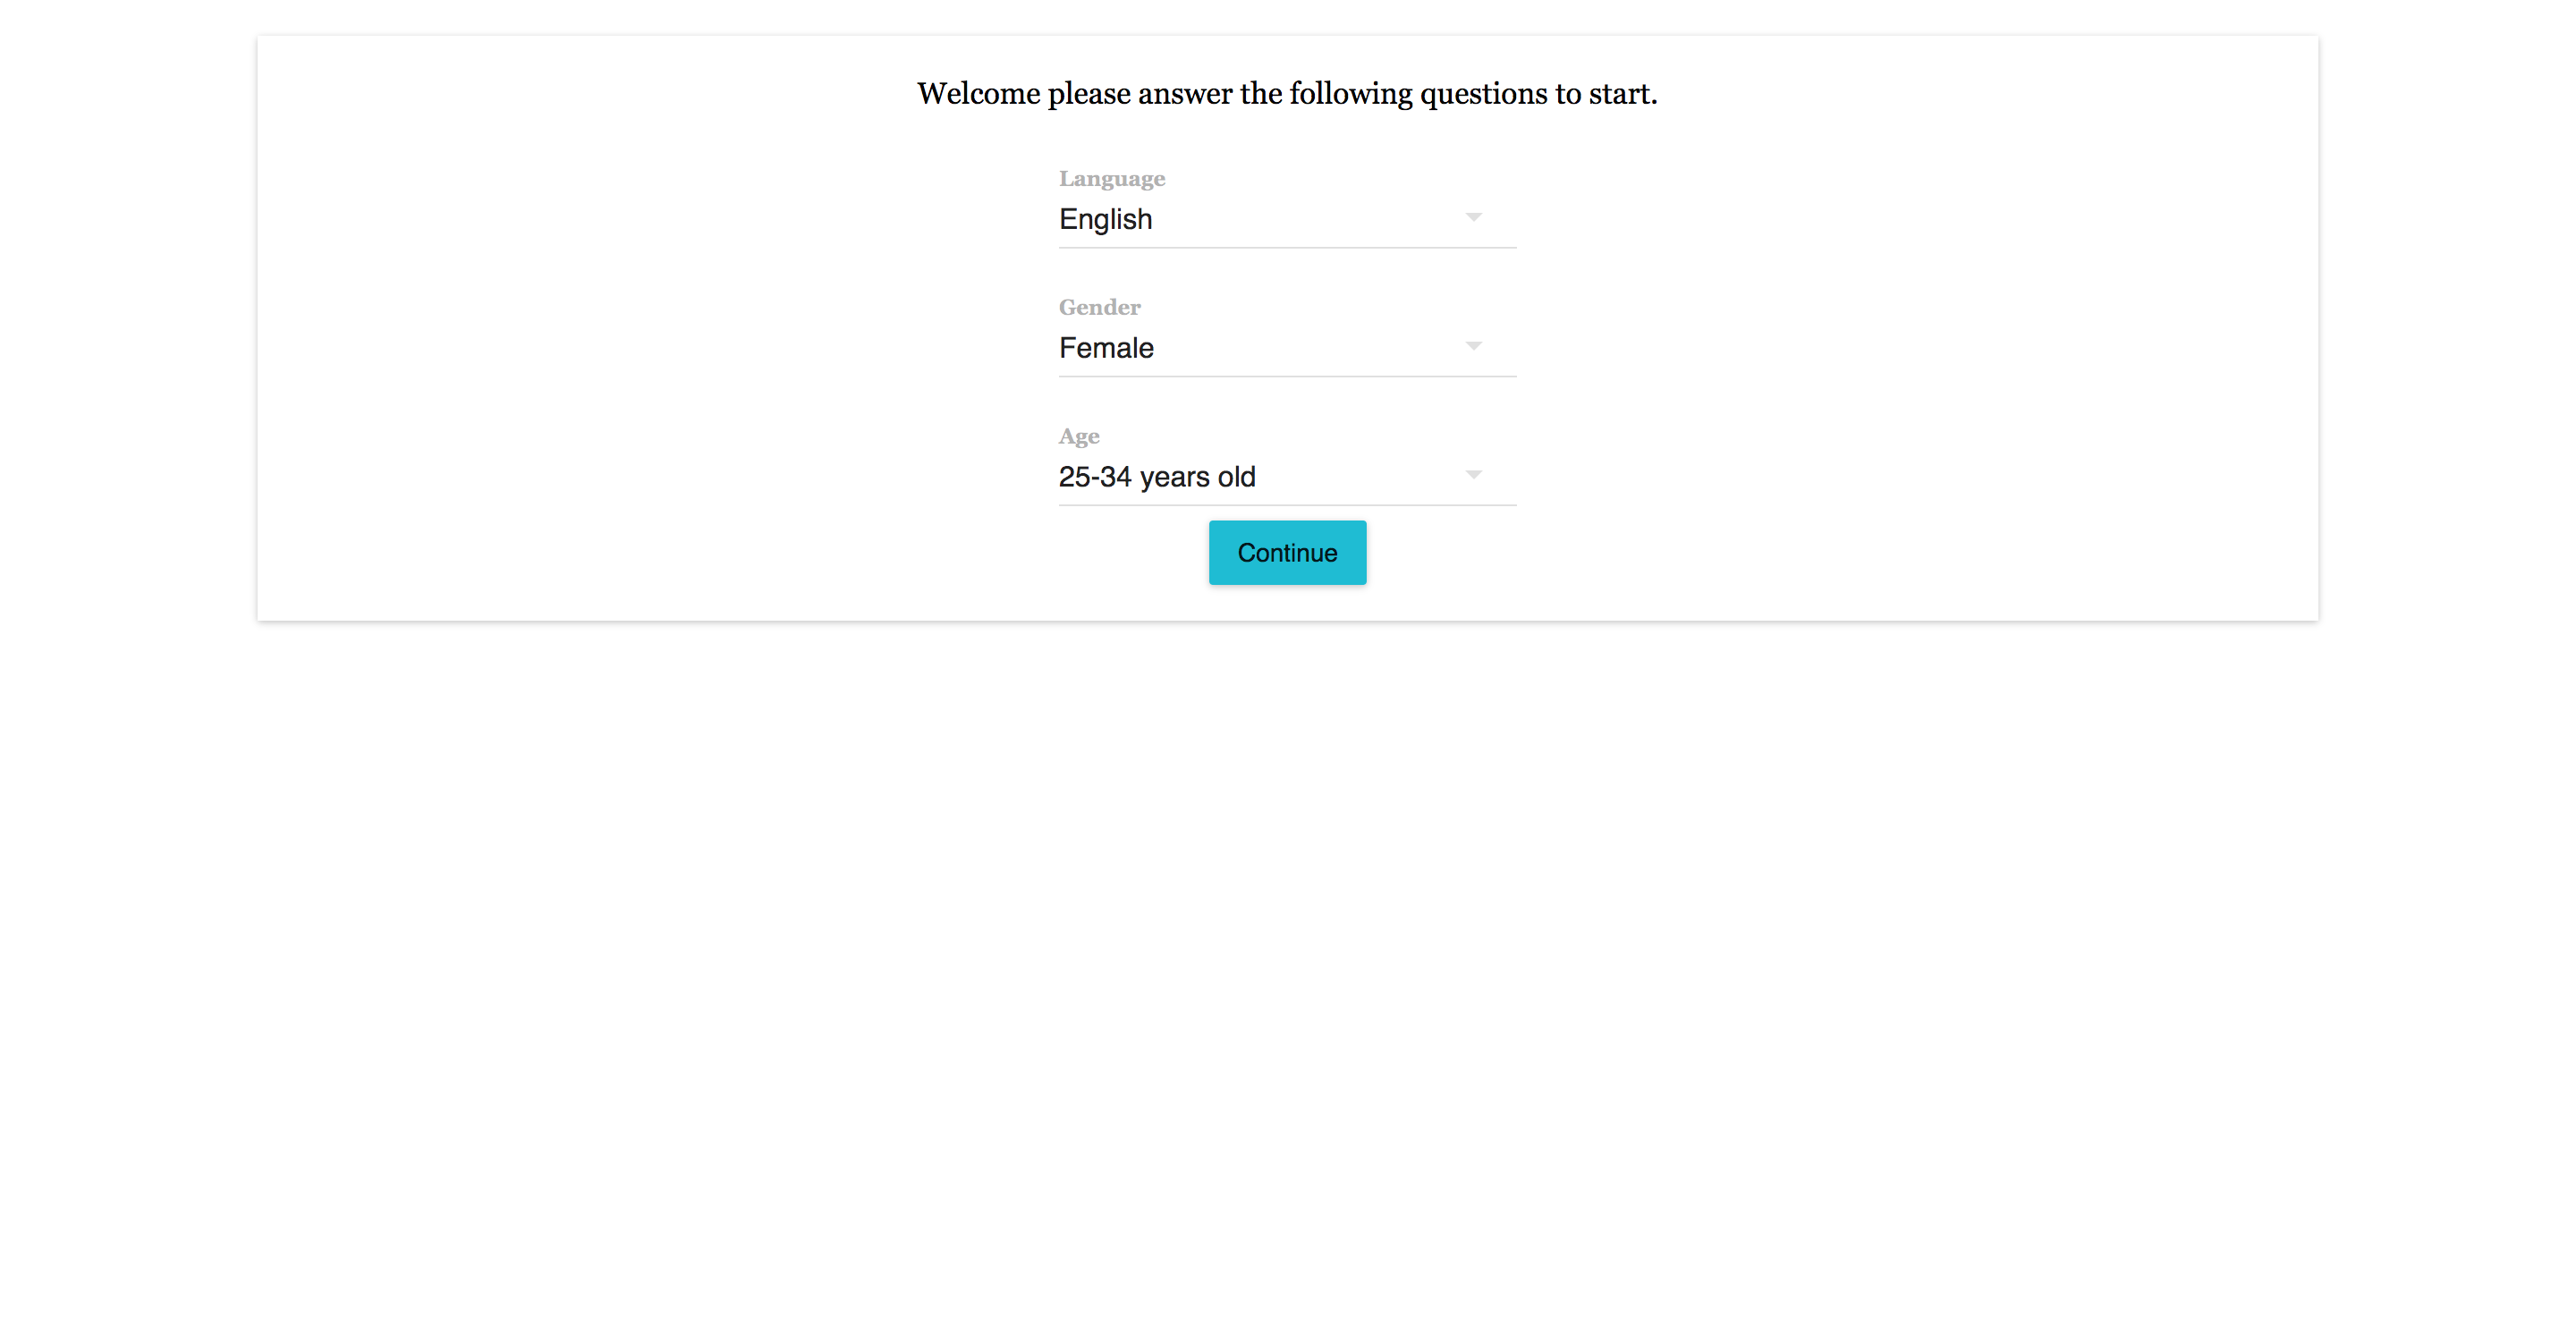
\includegraphics[width=100mm]{Images/homepage.png}
	\decoRule
	\caption[Homepage]{Image of the first page the user is greeted with. }
	\label{fig:homepage}
\end{figure}

\begin{figure}[h]
	\centering
	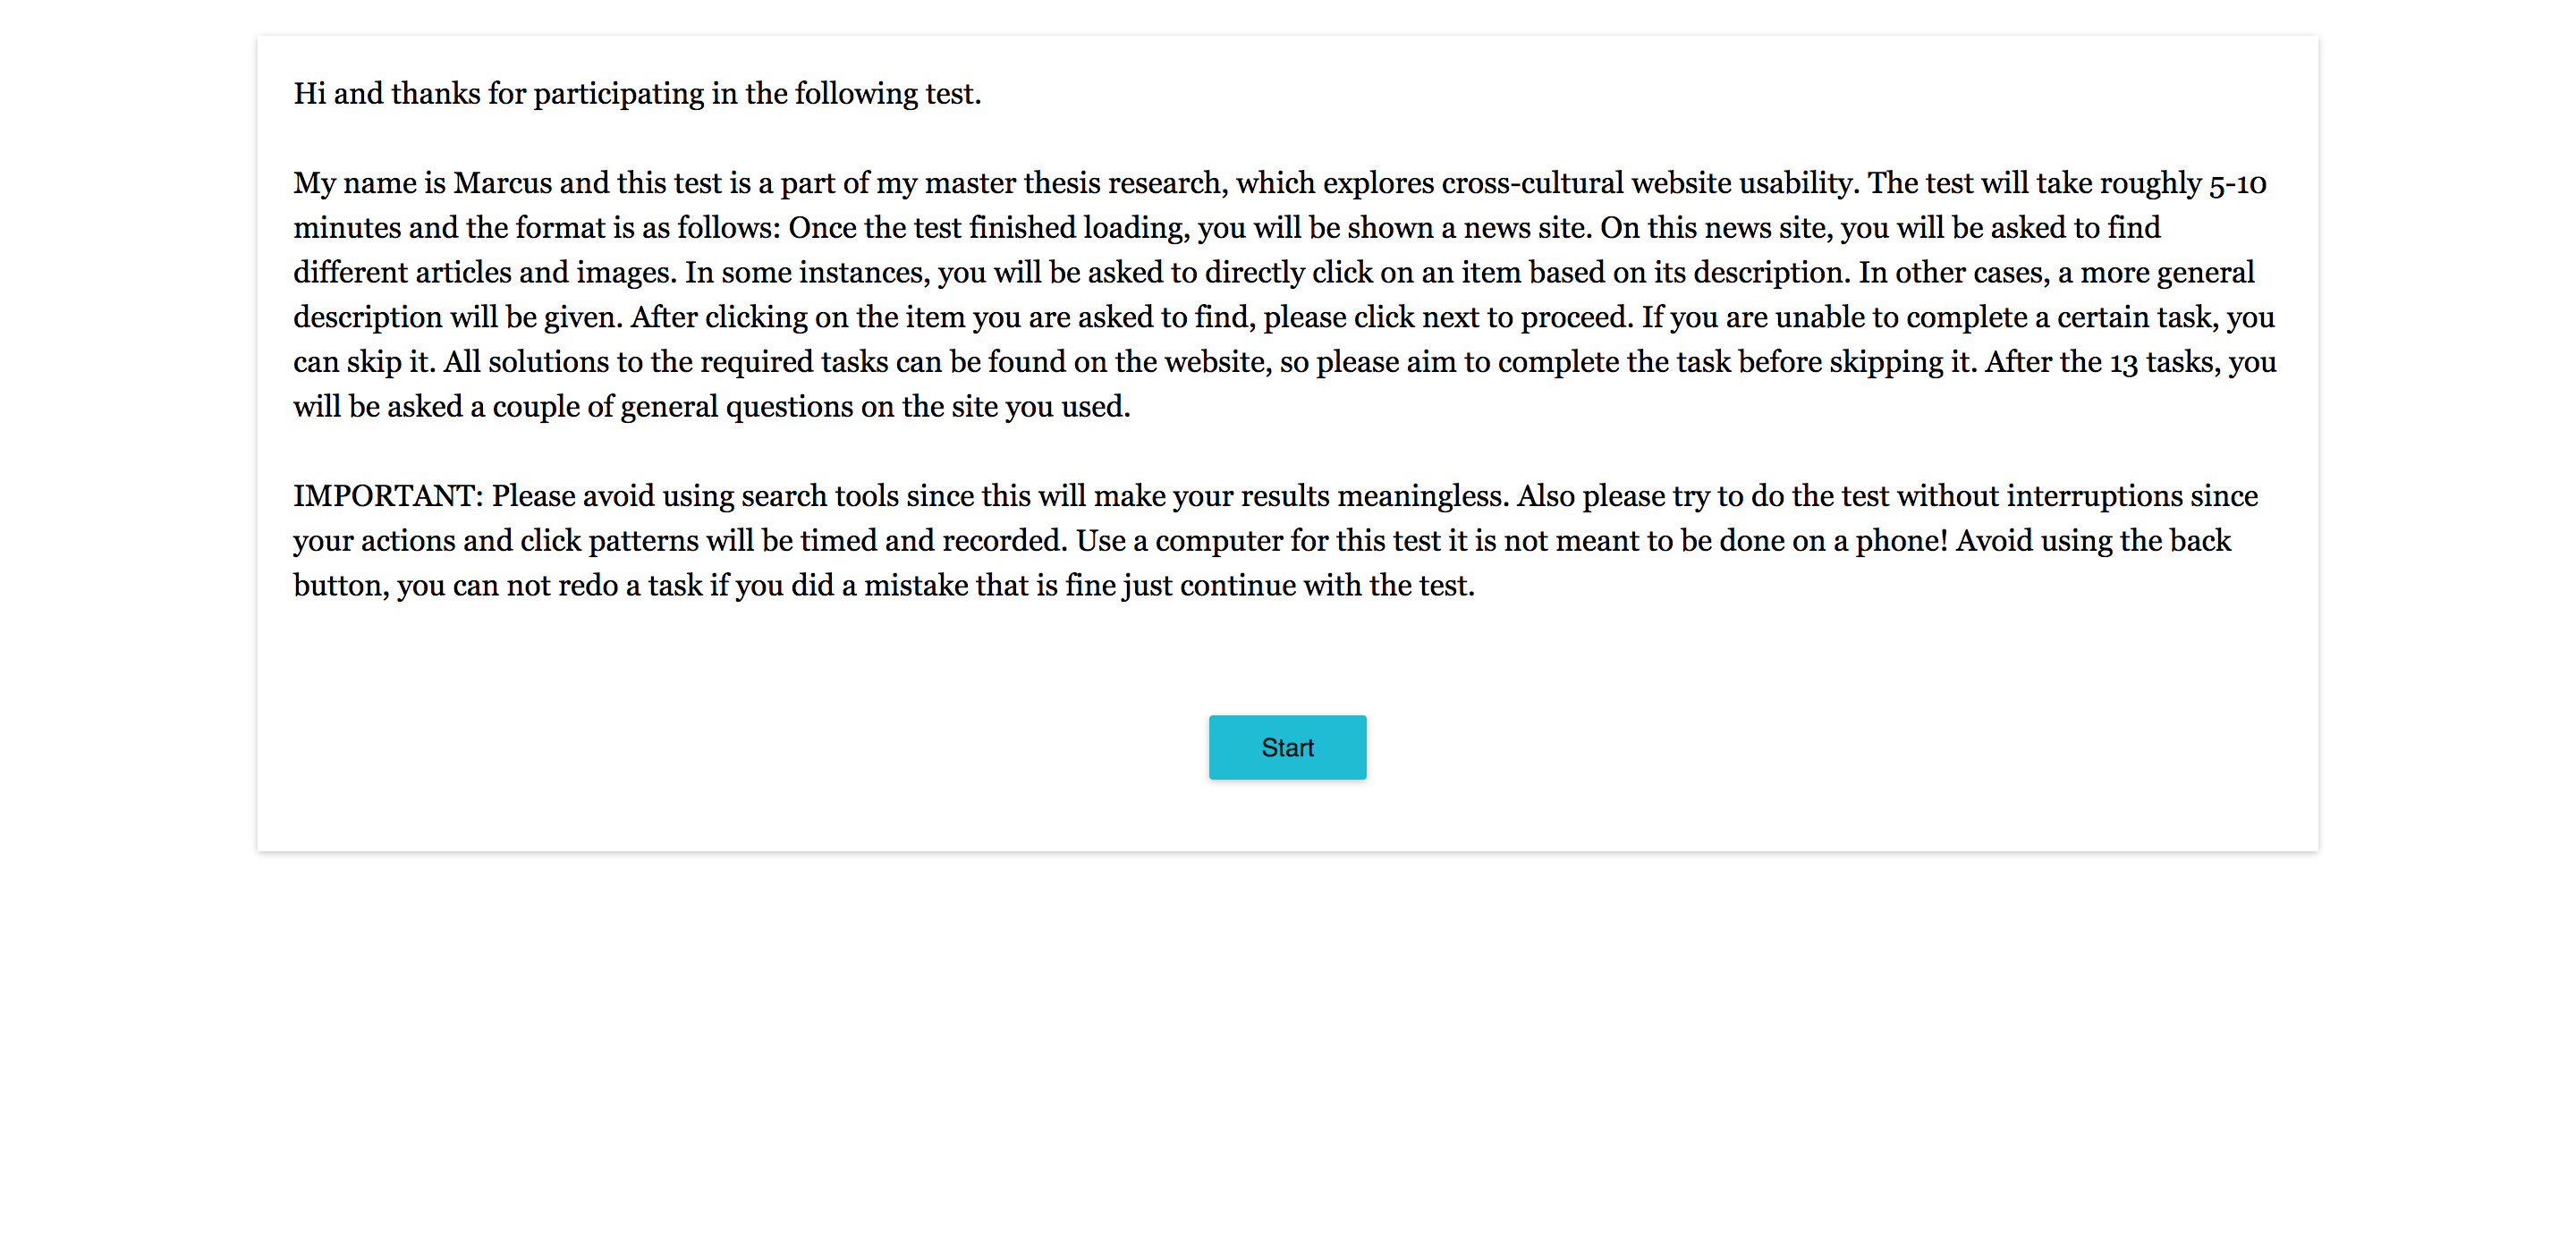
\includegraphics[width=100mm]{Images/homepage_text_en.png}
	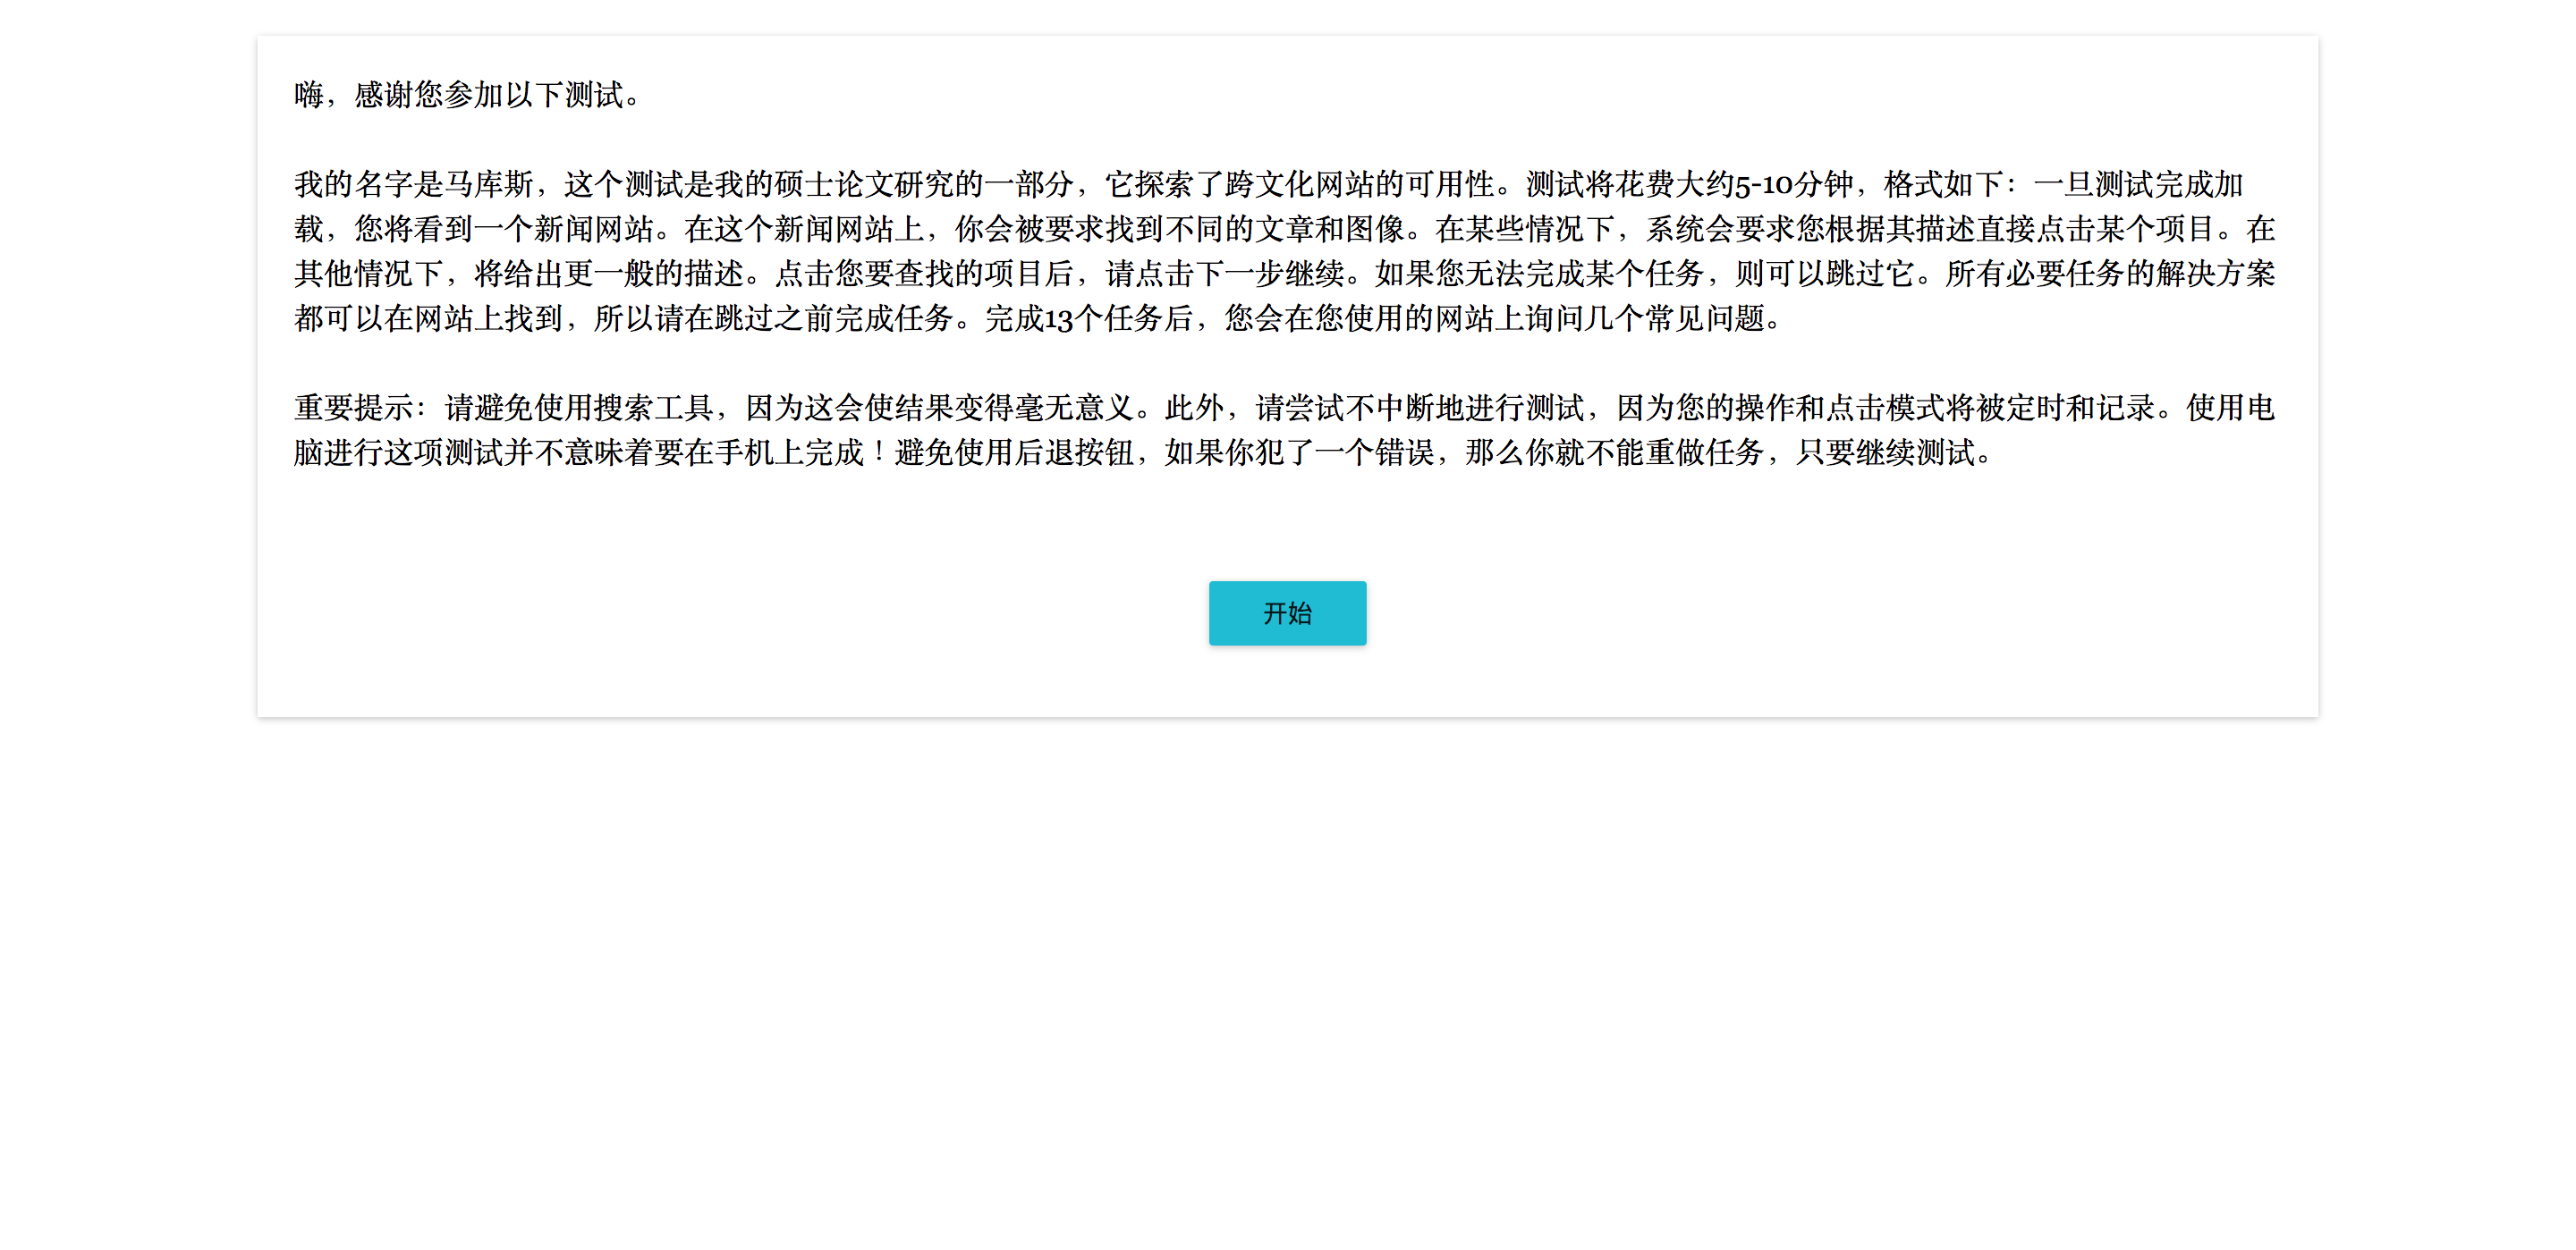
\includegraphics[width=100mm]{Images/homepage_text_zh.png}
	\decoRule
	\caption[Homepage]{Description in chinese and english.}
	\label{fig:homepage_desc}
\end{figure}
\subsubsection{BBC and QQ}
Both the bbc and qq inspired sites have the same basic layout. When the user arrives at the page a pop-up will appear with a loading bar, this is to make sure the user can't start the test until all the images has been loaded from the server. When all the images have been loaded the user will be able to start the test (see ref....).  
\\\\
All the news in this test has been translated so they have both the English and Chinese versions available depending on what language the user selected from the Homepage. Once the user starts the test a timer starts, the user is not able to see this timer. Each click the user does is recorded, the time it takes to complete the task and if the user gets the correct task or not. The number of questions the user have left to complete is also shown. The questions and what the user has most recently clicked is shown in a bar at the bottom of the screen (see \ref{fig:user_view}). Once the user finishes the test their answers are sent to the database via the API and they are redirected to the SUS site. 
\begin{figure}[h]
	\centering
	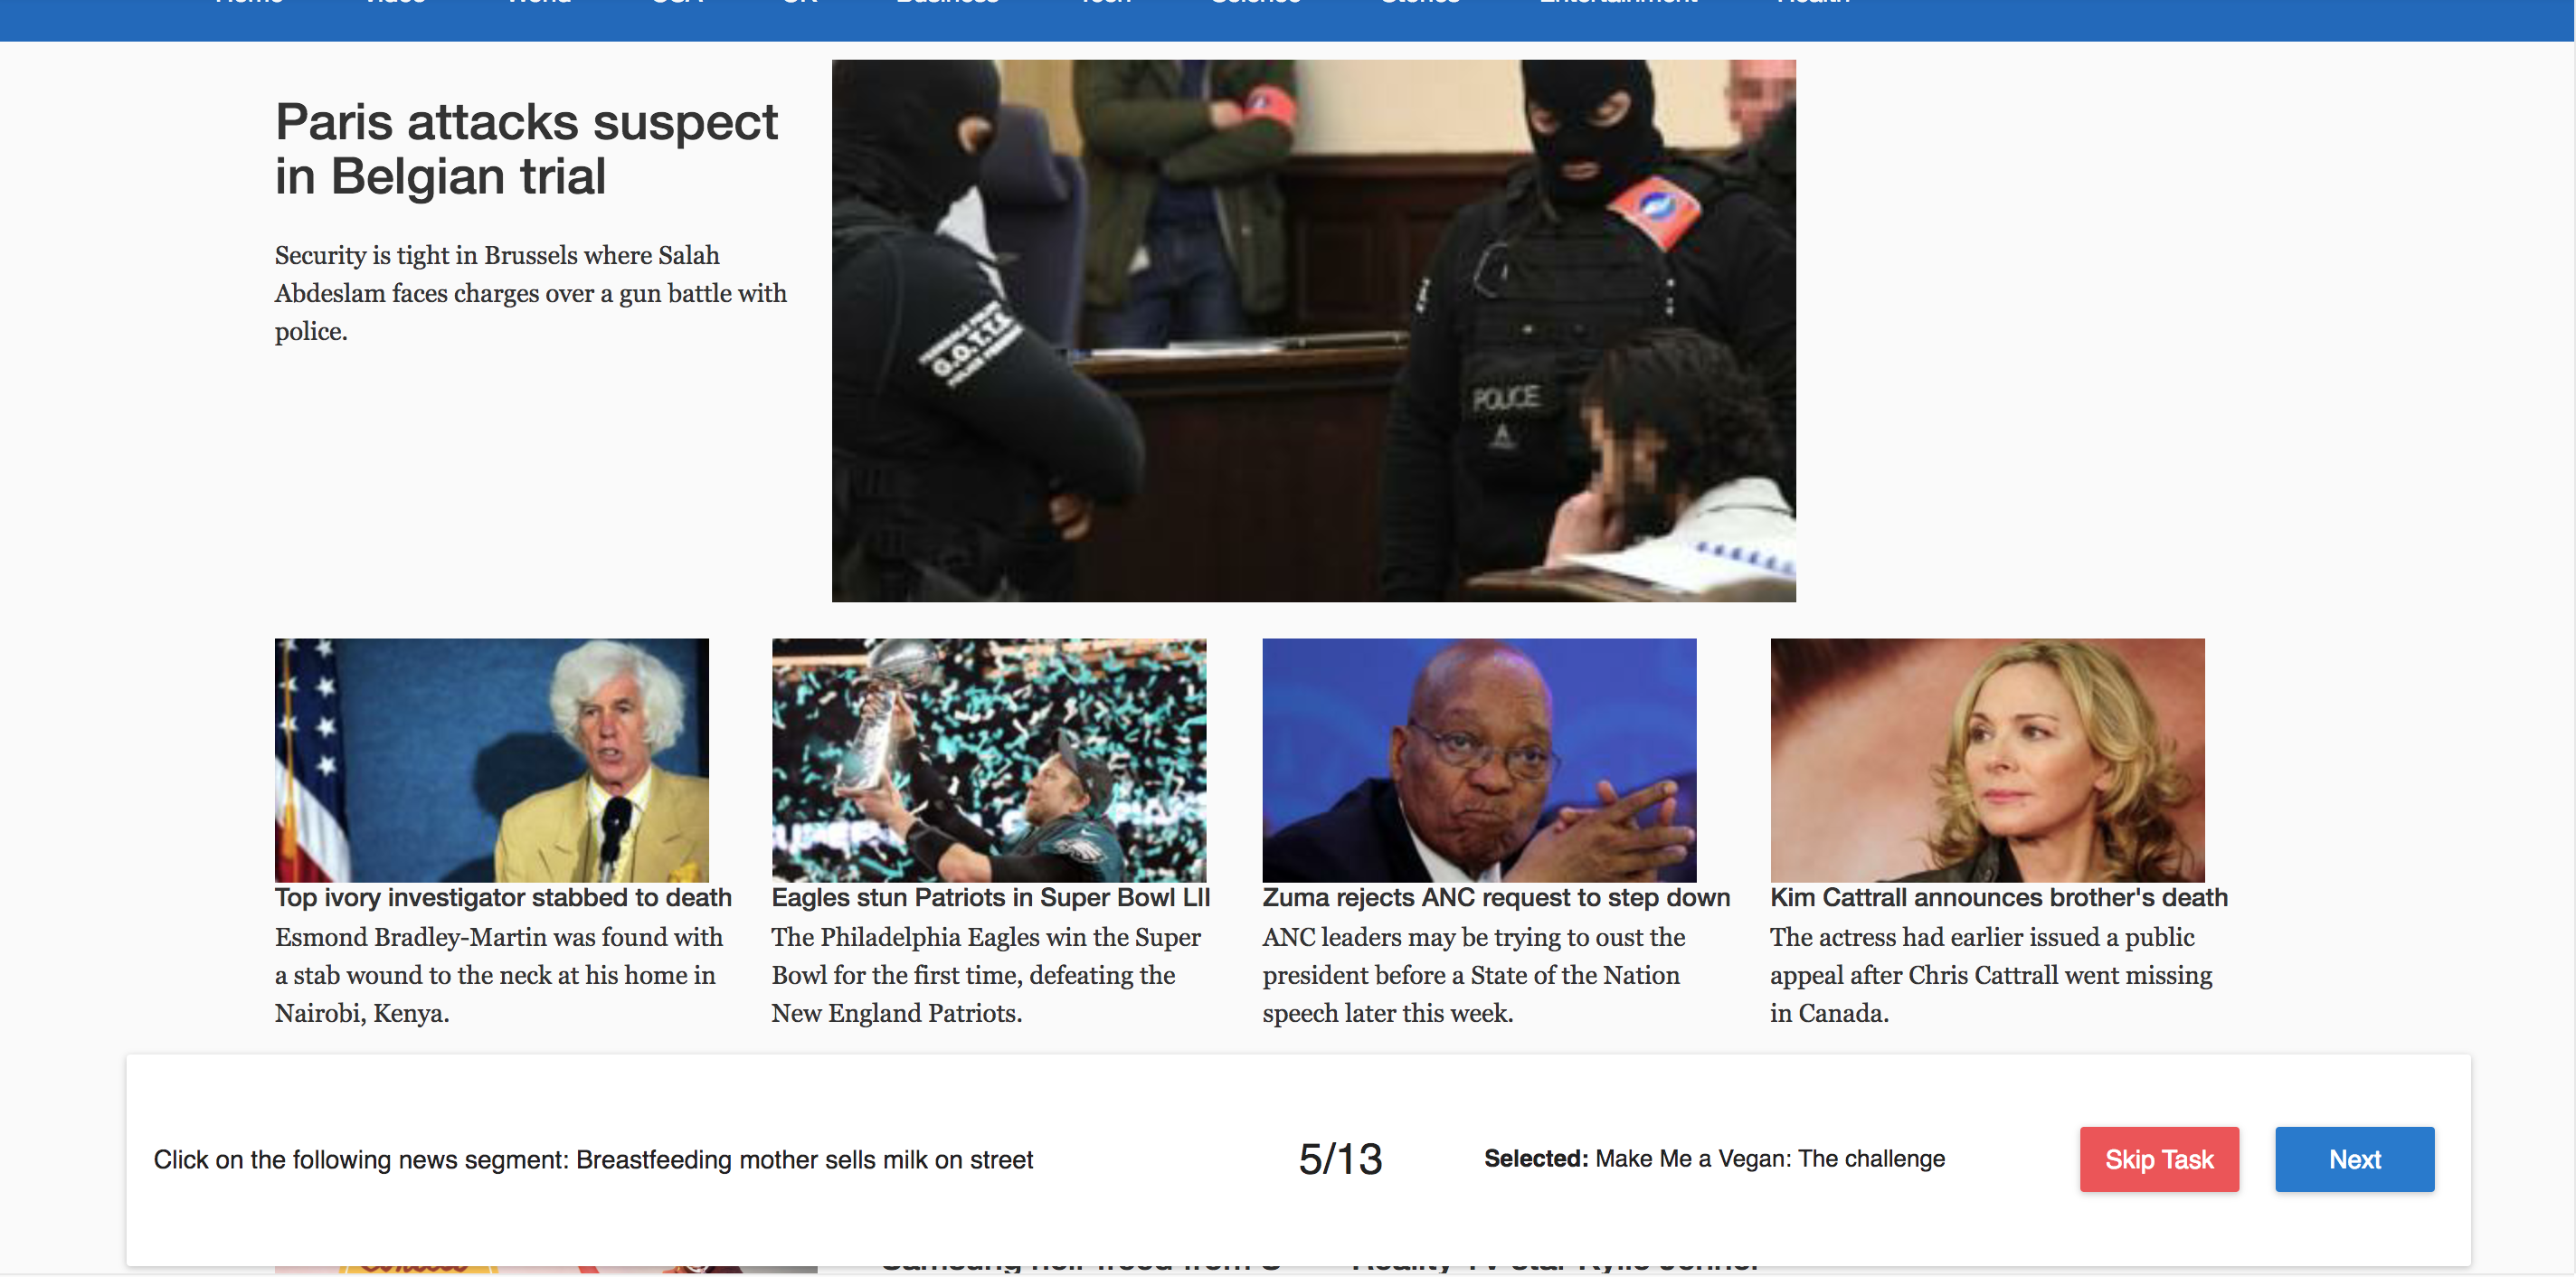
\includegraphics[width=70mm]{Images/view_bbc.png}
	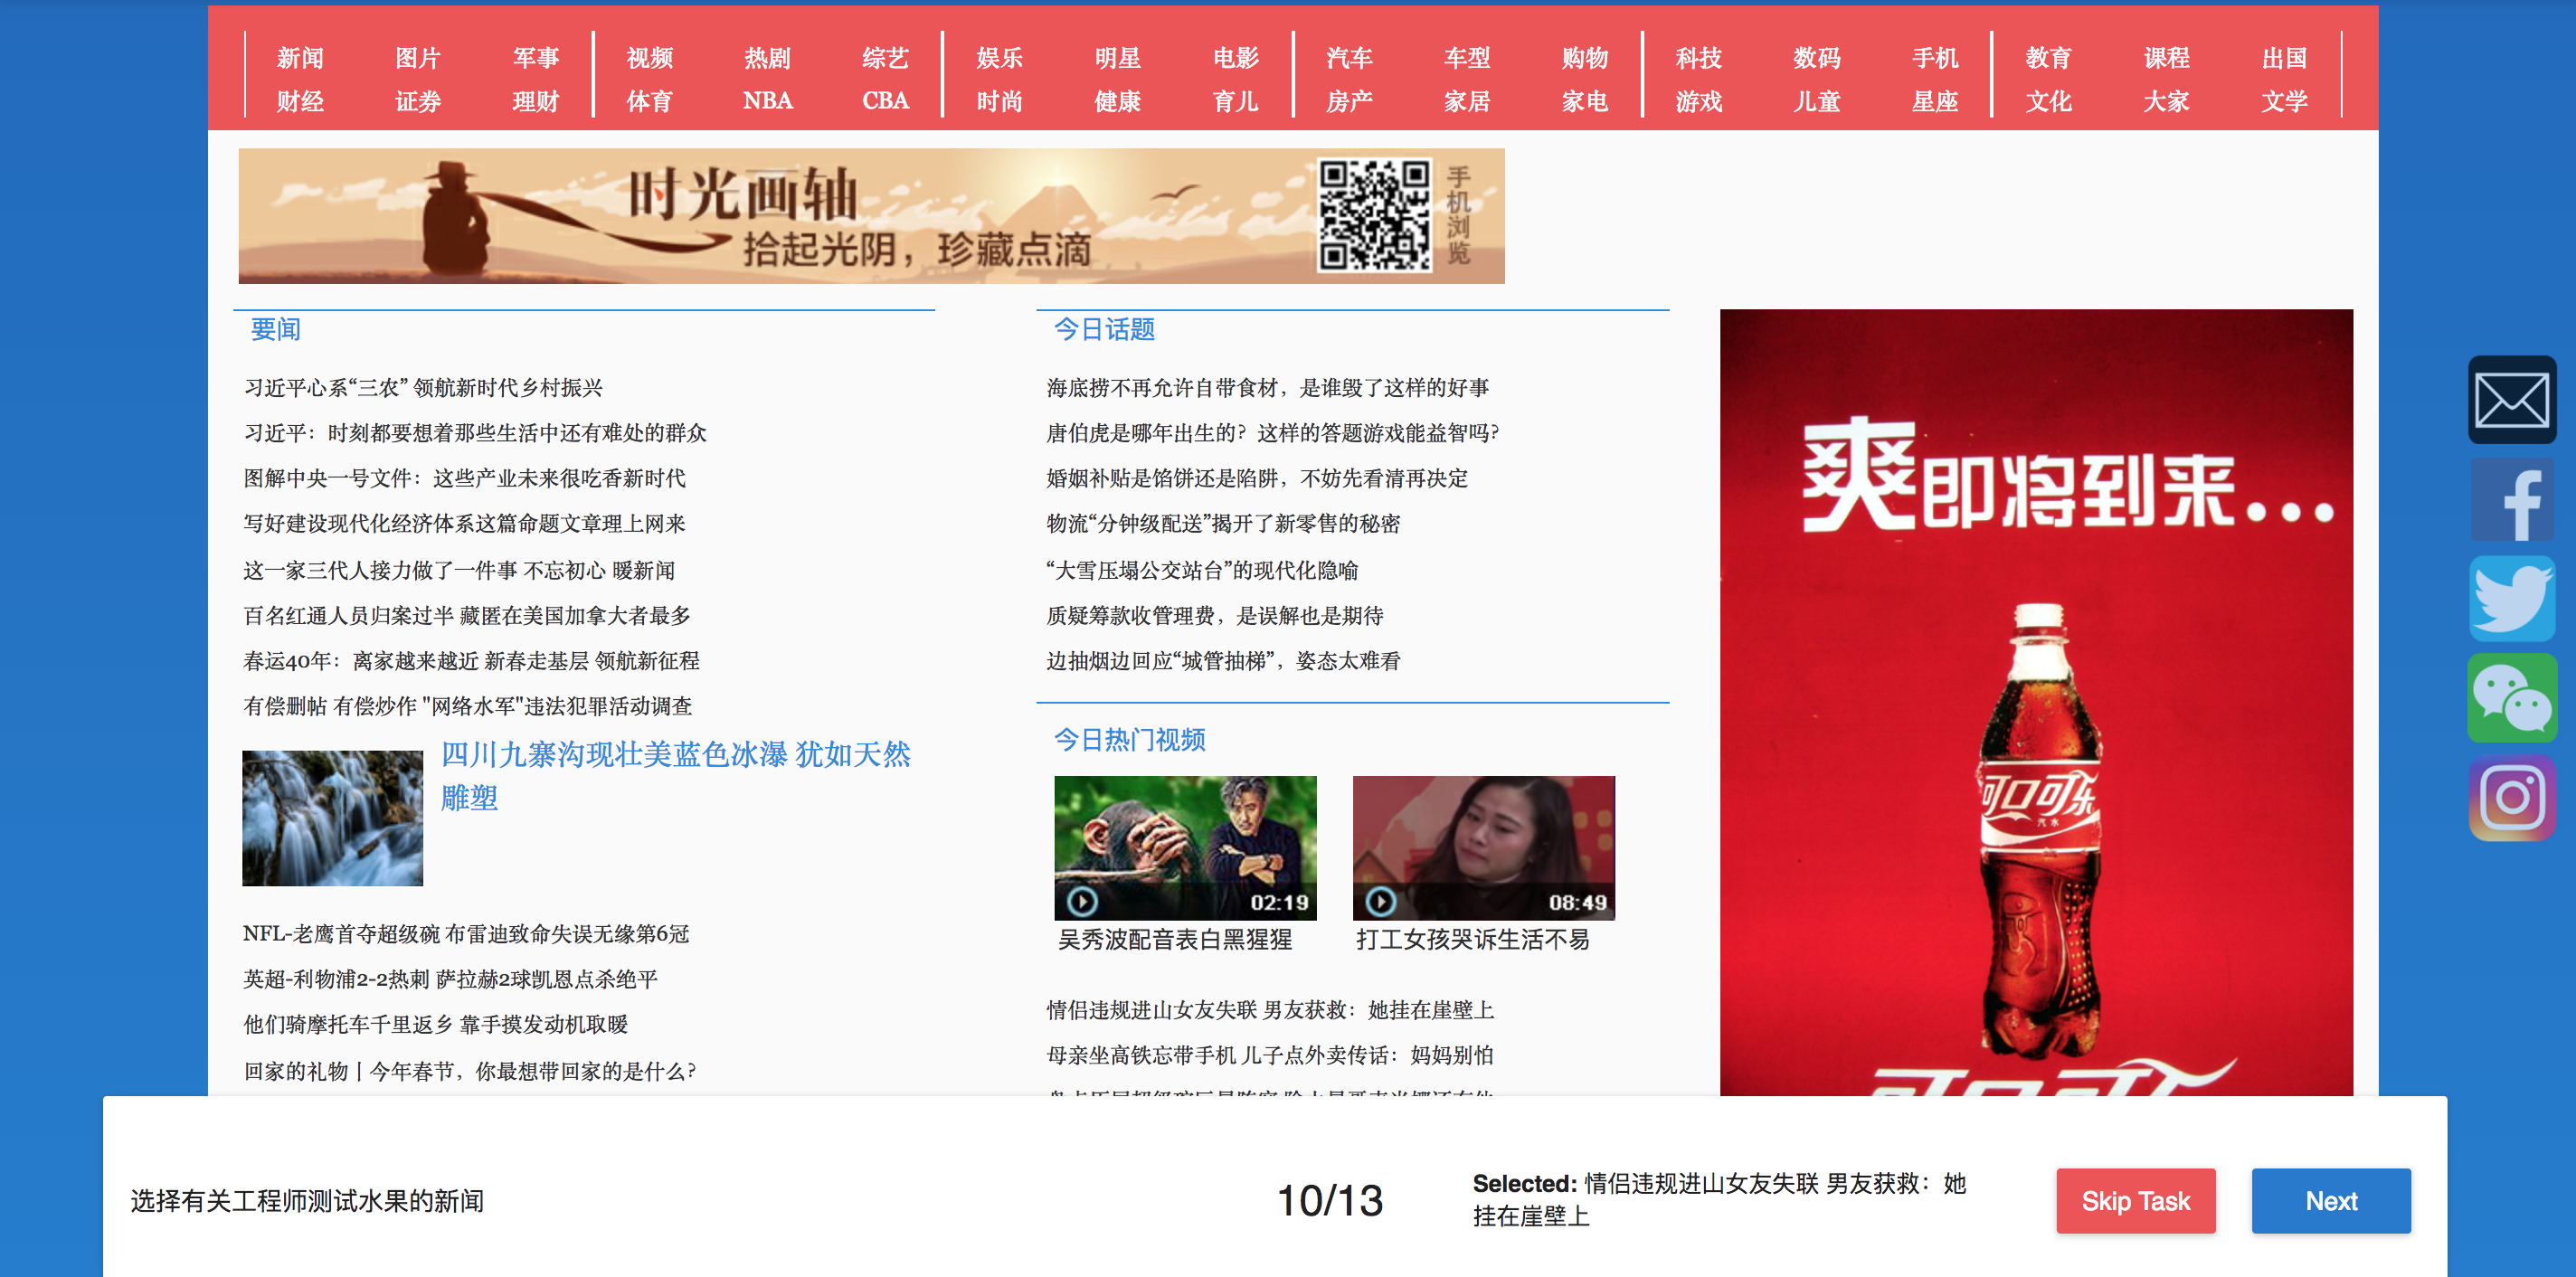
\includegraphics[width=70mm]{Images/view_qq.png}
	\decoRule
	\caption[Users View]{A example of what it might look for a user when testing bbc and qq inspired websites.}
	\label{fig:user_view}
\end{figure}
\begin{figure}[h]
	\centering
	\includegraphics[width=70mm]{Images/qq_site_zh.png}
	\includegraphics[width=70mm]{Images/qq_site_en.png}
	\decoRule
	\caption[QQ]{The full view of QQ site in english and chinese}
	\label{fig:qq_site}
\end{figure}
\begin{figure}[h]
	\centering
	\includegraphics[width=70mm]{Images/bbc_site_zh.png}
	\includegraphics[width=70mm]{Images/bbc_site_en.png}
	\decoRule
	\caption[BBC]{The full view of BBC site in english and chinese}
	\label{fig:bbc_site}
\end{figure}


\subsubsection{SUS}
This site consists of the before mentioned predefined questions designed to get a understanding for what the user fleet about the website, test and design (See fig \ref{fig:sus_site}). Once the user has answered all the questions and pressed finish their answers will be sent to the database via the api. The user will then be rerouted to the done site where they will see a message thanking them for participating in the test (See fig \ref{fig:done_site}).


\begin{figure}[h]
	\centering
	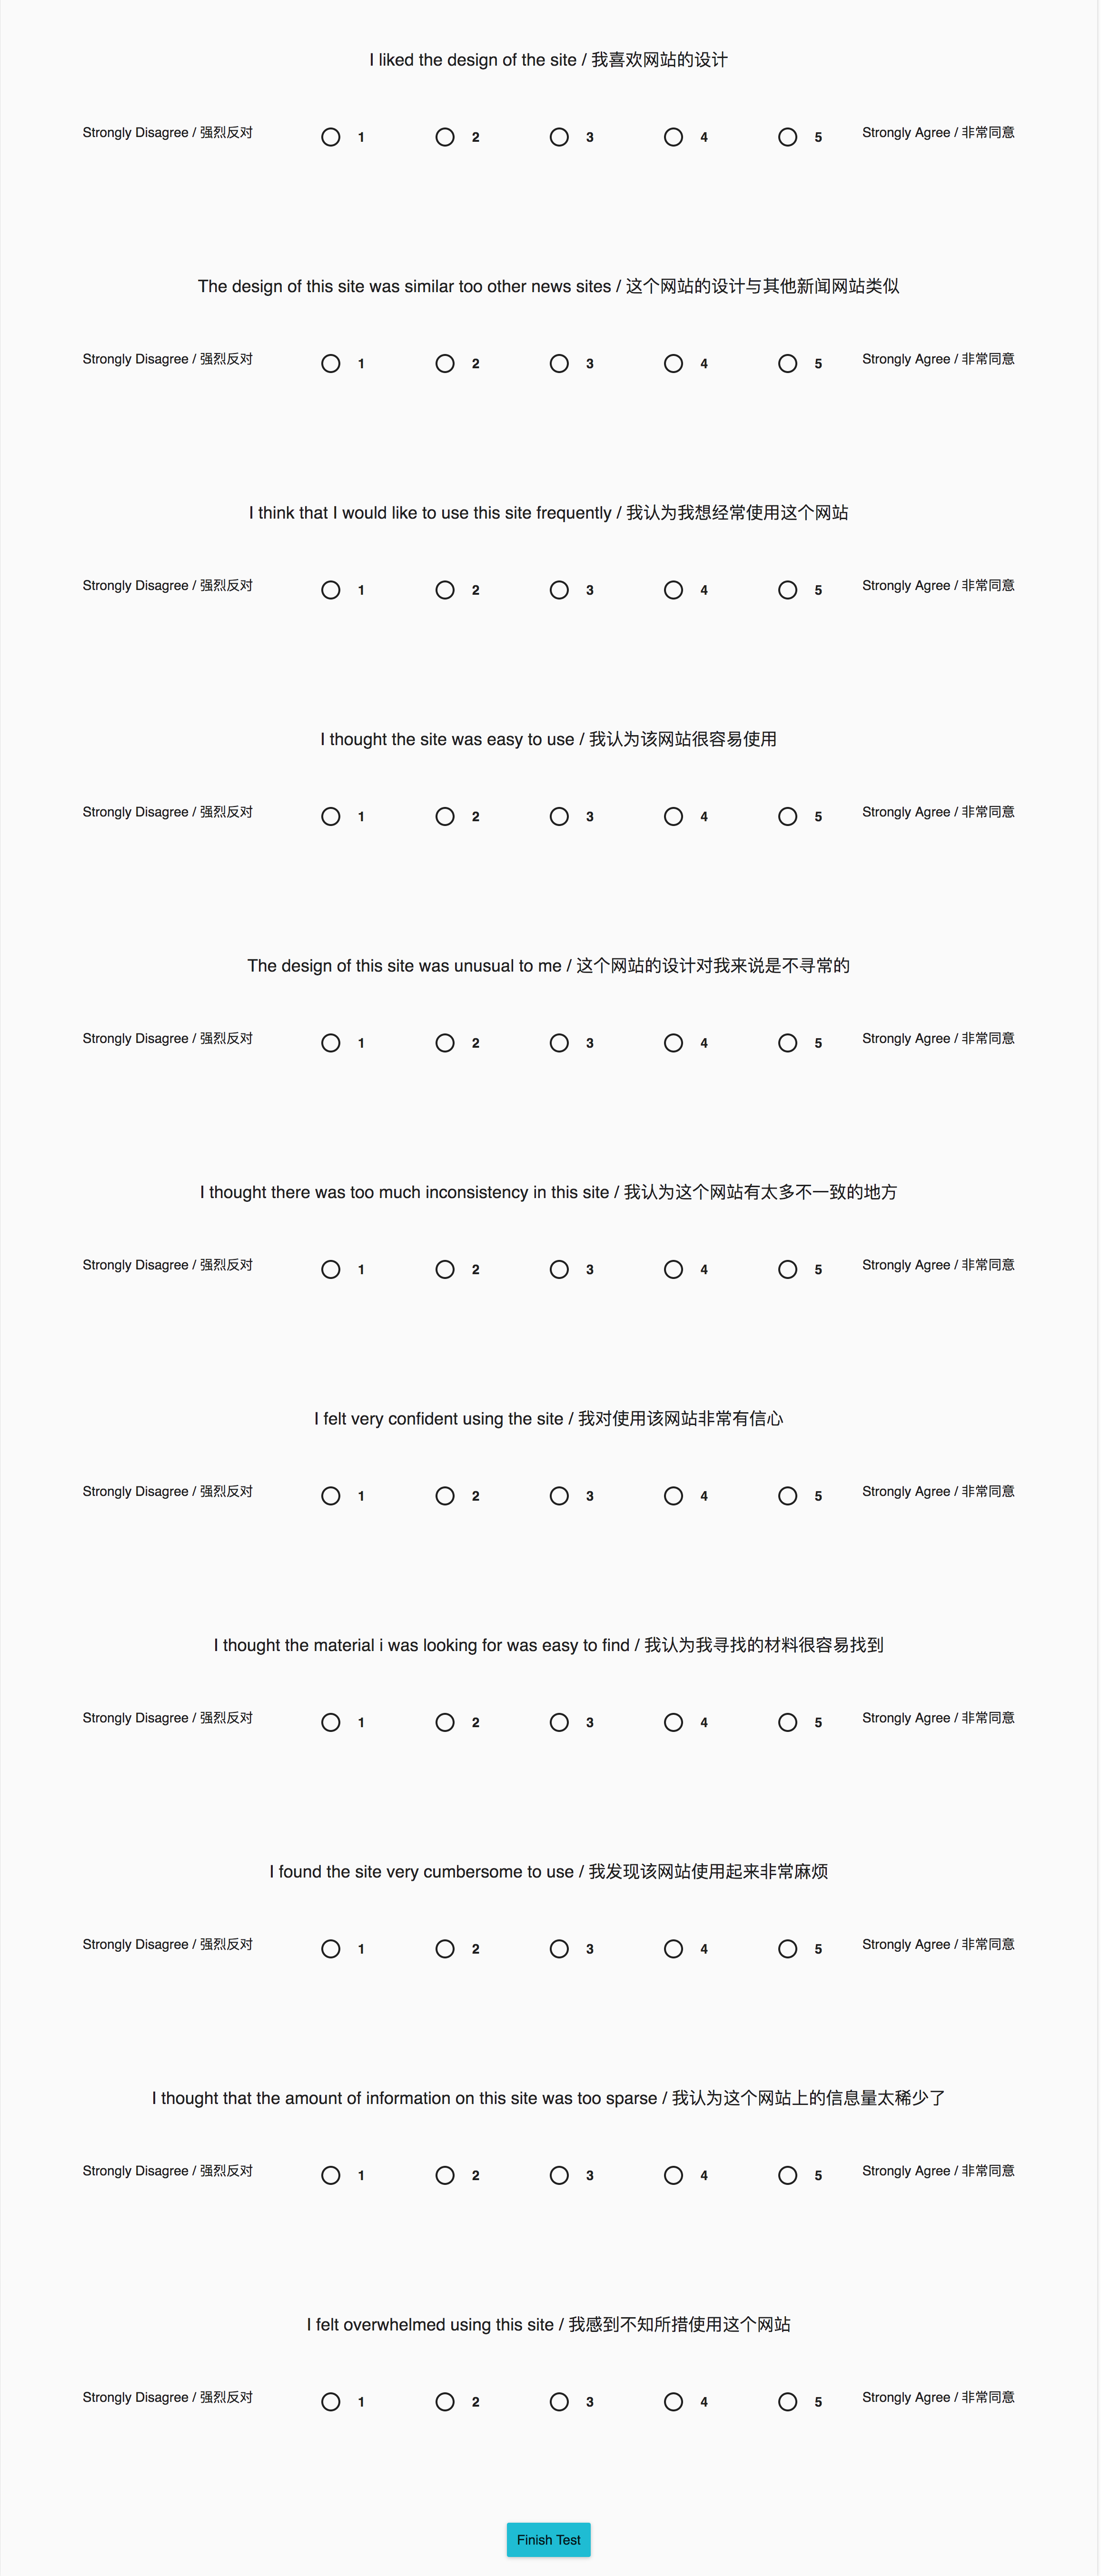
\includegraphics[width=70mm]{Images/sus.png}
	\decoRule
	\caption[SUS]{The sus site}
	\label{fig:sus_site}
\end{figure}
\begin{figure}[h]
	\centering
	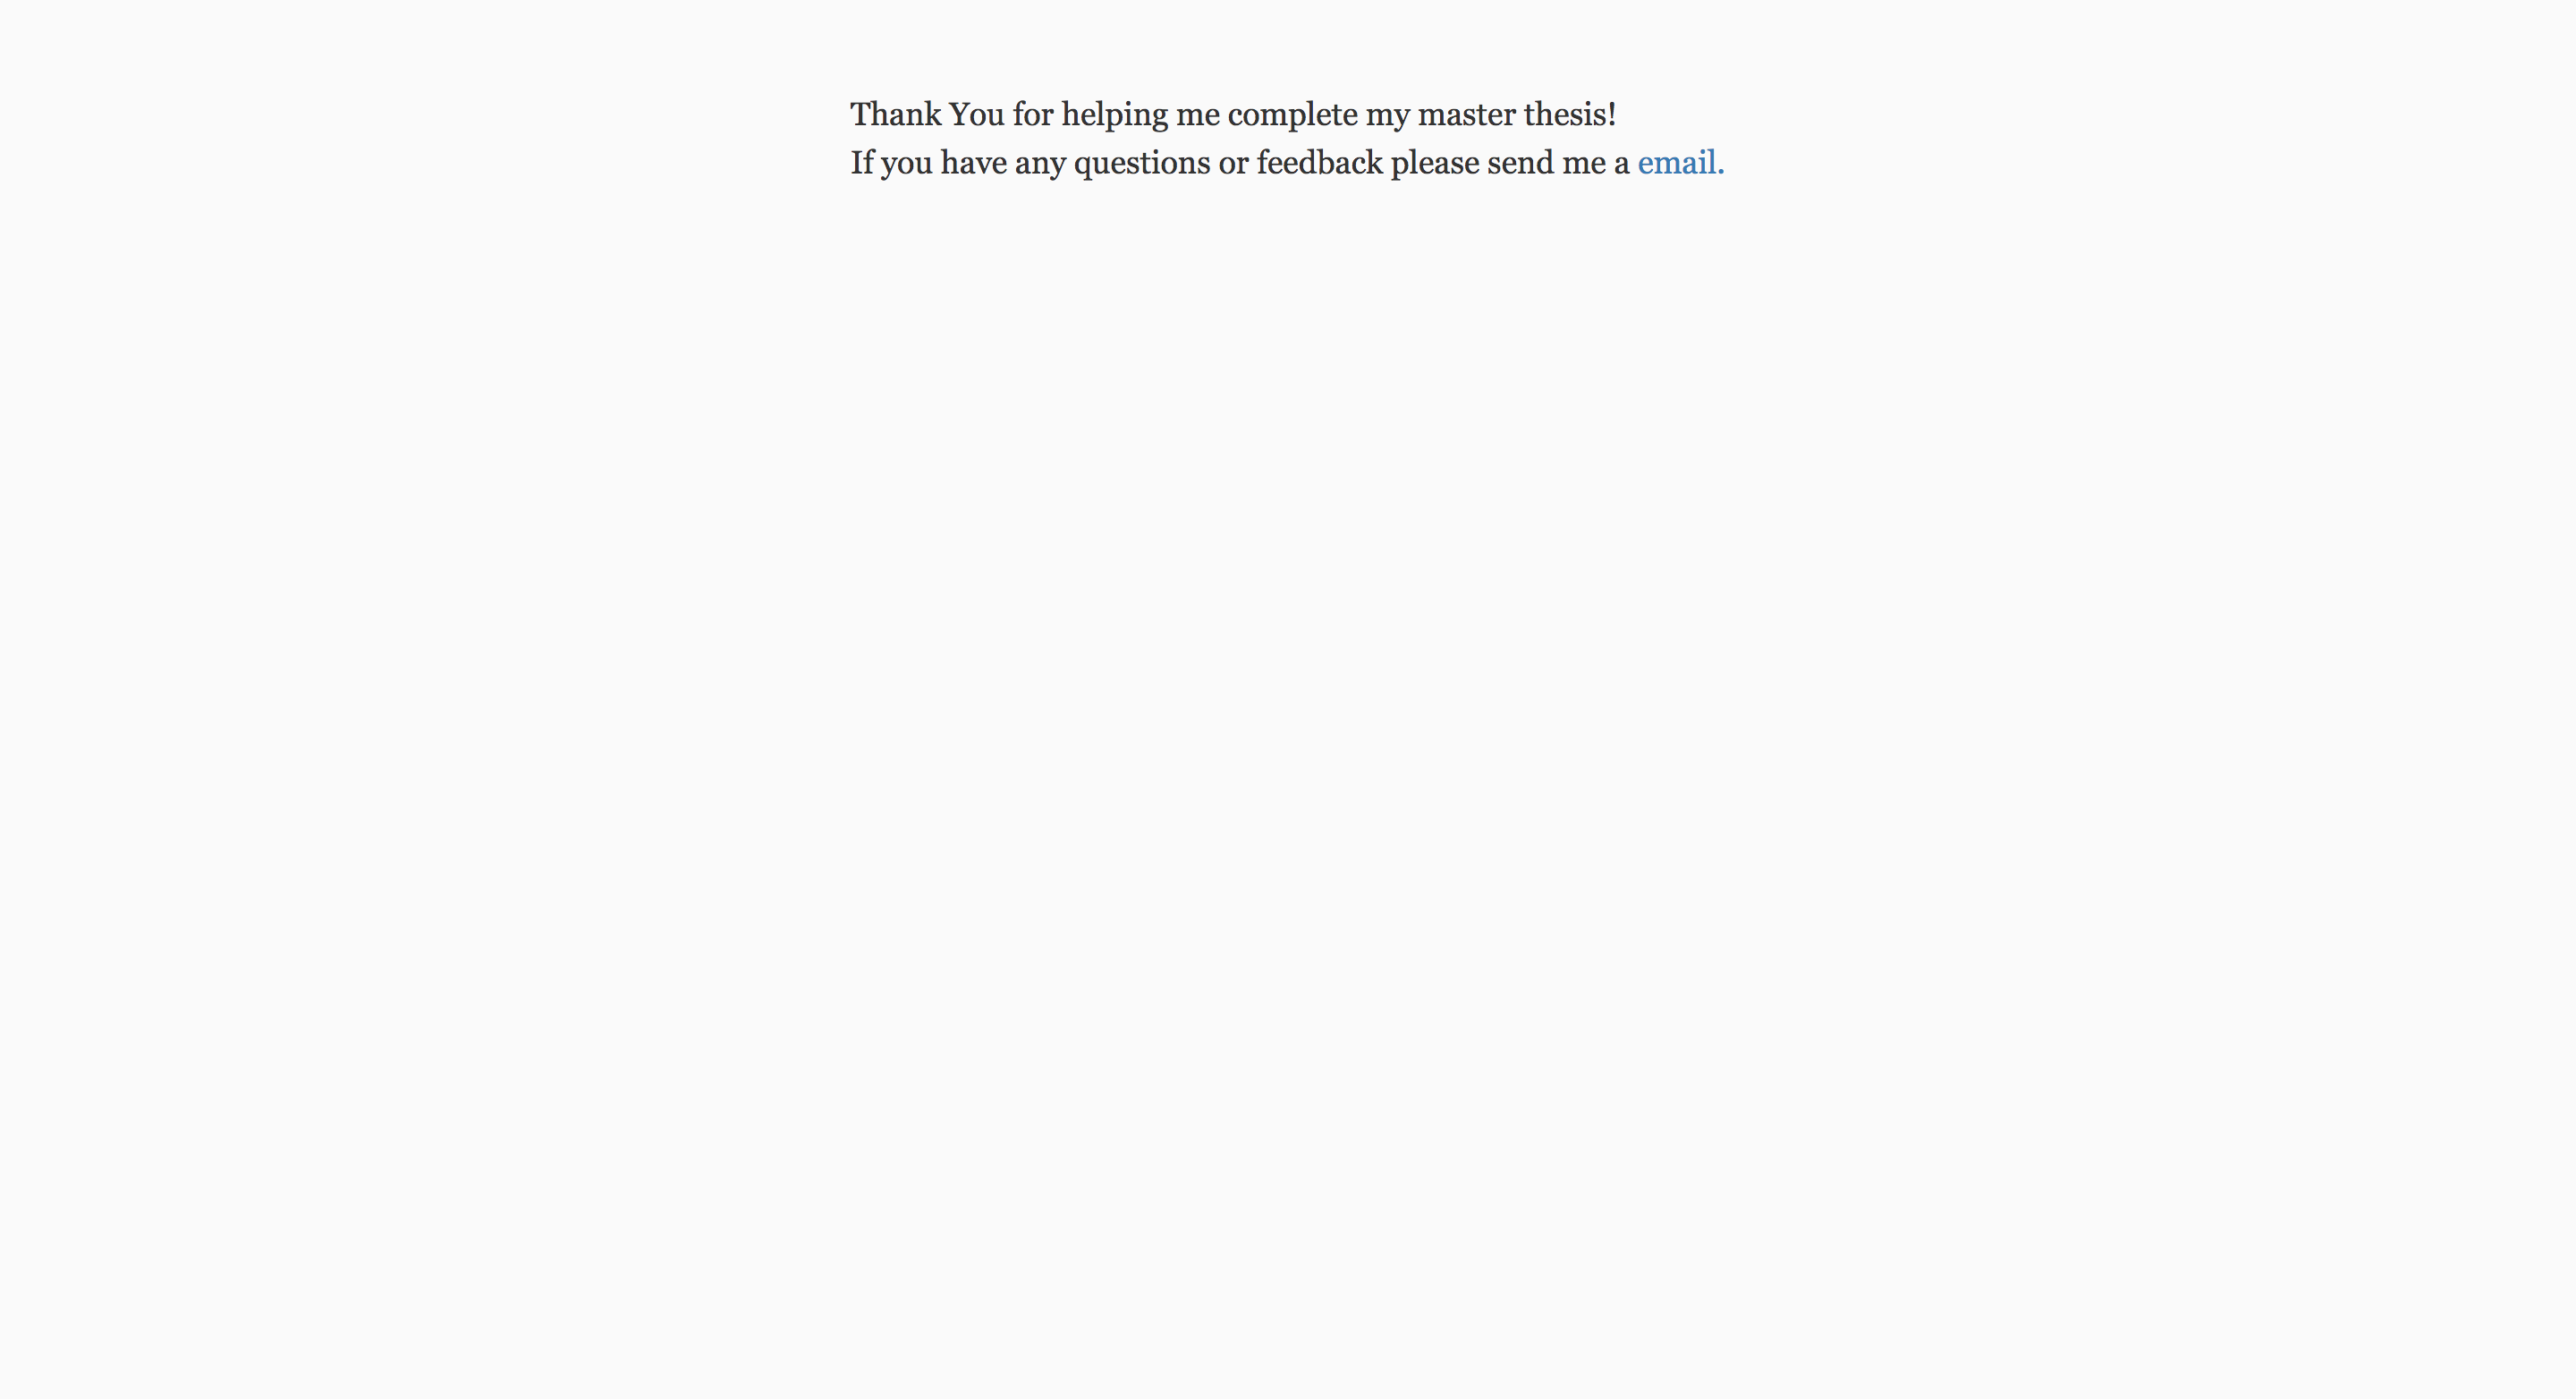
\includegraphics[width=100mm]{Images/done.png}
	\decoRule
	\caption[Done]{Last site the user is shown when they have finished the test. }
	\label{fig:done_site}
\end{figure}


\subsection{Database}
The database consists of five diffrent tables: Main, Actions, Questions, Sus and QuestionTexts. (See fig: \ref{fig:db_schema} for figure of the full database) 
\\\\
The Main mainly is used to identify the user where each user has a unique row. The table has four columns Id, Site, Language and Age. The id in the main table is the main id to identify a user. This same id can be found for each user in all other tables except QuestionTexts. 
\\\\
The Questions table contain all the answers from the users, the table has seven columns: Id, MainId, QuestionId, Correct, StartTime, EndTime, Correct, TotalTime. MainId and QuestionId is foregin keys referencing the ids in the Main and QuestionsTexts tables.
Each row in the Question table contain a answer from a user.
\\\\
The Action table contain all the click-actions a user did per question. The table contain seven columns: Id, QuestionsId, PosX, PosY, ScreenWidth, ScreenHeight, RelativeTime. Where QuestionsId is a foregin key referencing the Id in Questions. Each row in the Action table contain a action made by the user.
\\\\
The Sus table simply contains all the users answers to the Sus questions. The QuestionTexs table contain all the questions the user are asked in the test

\begin{figure}[h]
	\centering
	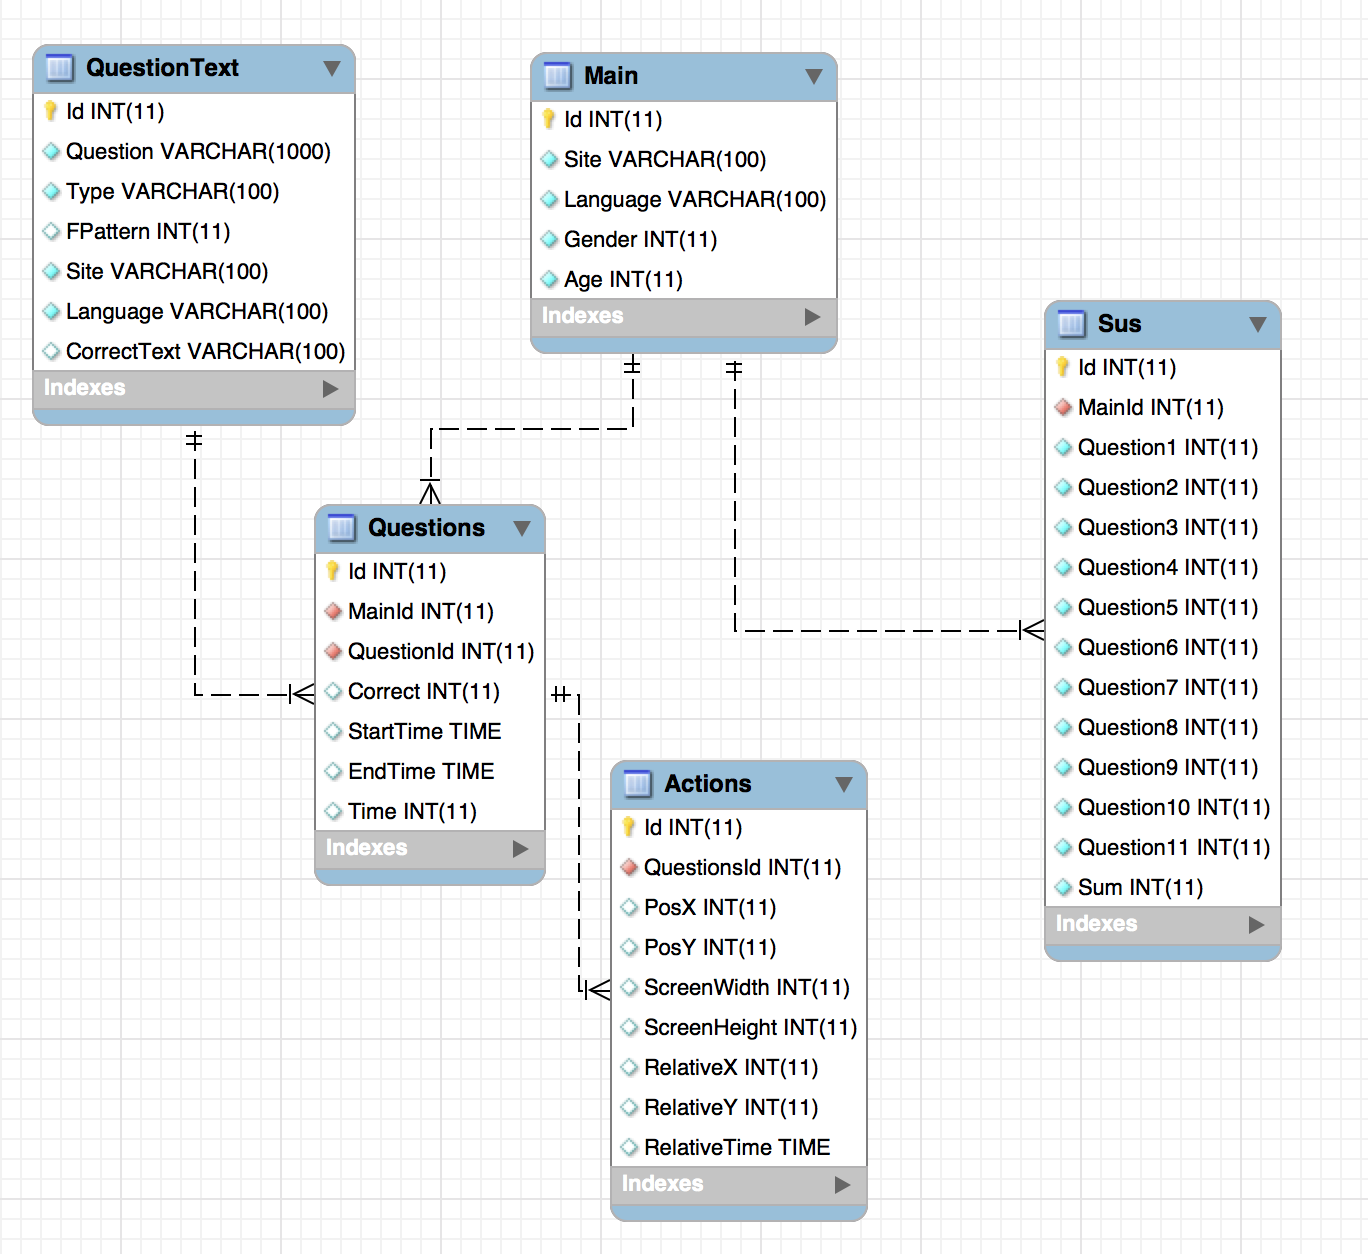
\includegraphics[width=100mm]{Images/db_eer.png}
	\decoRule
	\caption[Database Schema]{A EER schema of the mysql database. Yellow icons show the tables primary key, red the foreign keys and blue/white the atributes.}
	\label{fig:db_schema}
\end{figure}

\subsection{Api}
A express Api was set up to handle communication between the front-end and database. The Api takes the information that is sent from the users front-end code and transform it into a format that works for the sql database. The Api then quires the database and insert the new data into the database tables.

\subsection{Hosting AWS}
To host this app on AWS we used the feature called "Elastic Beanstalk" also called eb. Eb allowed us to easily launch a application that automatically set up a EC2 instance, auto scaling, load-balancing, RDS. The services was set up in Seoul. This to decrease the loading time for China as much as possible. Since Seoul also have very good network connections to the rest of the world this does not increase the loading time in Europe and the US that much. A lot of time had to be spent changing parts of the code so it would run on AWS servers.

\subsection{Beta-tests}
Once a working version of the test was created. A beta test was made to find possible bugs in code and improve user-experience in terms of font-size and design of the testing parts.
The beta-tests where made in the form of letting users try to finish the test while It was supervised. Notes where taken about possible misunderstandings, bugs and improvements that could be made to the test. Some examples of notes that was taken during the beta tests can be seen below. 

\begin{enumerate}
	\item Make selected bigger so the user can easier see what they have done.
	\item Should we log scrolling?
	\item Some correct question gets logged as incorrect in database in-spite of being correct.
	\item Waiting for sus site is very slow. Is it waiting for the database?
	\item Left top-side of qq site is too small, because of commercial?
	\item Wrong spelling in some news.
	\item Skip task not working.
	\item Some correct question gets loged as incorrect in database in-spite of being correct.
	\item Change so the size of the page is constant no matter the screen size. (Looked very bad on a big screen right now.)
	\item Start time not working correctly on some questions.
	\item Remove video from questions, does not give any relevant information.
\end{enumerate}

The beta was tested on about ten people where six did the English version of the test and four the Chinese version. After about eight tests almost no new information about usability problems and bugs where found so it was concluded to finish the beta testing and launch the test.

\subsection{Launch}
The launch of the test when fairly quickly with AWS. During the launch the performance of the site was monitored closely and we could thereby see that loading times increased when several people used the site at the same time and not all results where logged in the database. It was quickly concluded this was beacuse a problem with the database connection from the api and within the matter of minutes this bug was fixed and the site was updated. It can be estimated that about 4-5 test results where lost due to this mistake.

\subsection{How the test was conducted}
it was sent out so only one test person did the test once. No repeats of the test where made

\section{Results} (CHANGE)
We received quite a few responses from both English and Chinese users. In total we revived about 99 replies from people who did the test. 40 of these where from Chinese users and 59 from English speaking users. Of these users 61 where male and 38 female.  
 
 The majority of the test subjects are students studying at university. Most of the english speaking students are from Lunds University and the majority of the Chinese speakers are from xxxxx university in China. The rest of the test subjects are a mix of people from the Swedish and Chinese Tetra pak offices.
 The age of the test subjects are quite similar as can be seen in the graph below (/ref here for graph!).
 
(Bild från age grafen)
 

\section{Discussion}
The programing is the largest and most time consuming part of this thesis and there were several requirents of the code for the tests results to be useful. (OBS BORDE DHA MED ALLA REQUIREMTENTS NÅGONSTANTS. The requirements from the code can be seen in (REF TO REQ HERE). On top of previusly decided requirements the following where also added when it was realised that they where needed: 
 \begin{enumerate}
 	\item Users are not allowed to use ctrl-search
 	\item What site the user will test on should be controlled, this so we receive equal amount of tests for both sites.
 	\item 
 \end{enumerate}

The results are from the raw data. This means that the data will have to be cleaned before able to be used. Some examples of what have to be removed are: 

\begin{enumerate}
	\item Tests done on Phone
	\item Questions where the user has left the test.
	\item Tests where the user only skipped through all the questions
\end{enumerate}






\section{Conclusion}
Vad som behövde ändras efter beta, samt panik updatering på mysql databasen, hur vissa trots text försökte göra på mobil
 
% Chapter Template

\chapter{Phase 4 - Analyzing Data} % Main chapter title

\label{Chapter7} % Change X to a consecutive number; for referencing this chapter elsewhere, use \ref{ChapterX}

%----------------------------------------------------------------------------------------
%	SECTION 1
%----------------------------------------------------------------------------------------
The goal with this phase is to use the language python combined with mysql quires to get the data from the database. Clean the data and then analyse the results and test it for statistical significance.

\section{Work process}
The main technologies used for this phase was Python using several different libraries and mysql to querie the database in Seul, South Korea.

data gathering process:
To gather the data from the MySQL database several queries were made with conditions that specified what specific data to be gathered. This data then loaded into a data frame in python. Eight different data frames were created. Four containing information about the user's actions on each question these were the following: English speaking BBC users,  Chinese BBC users,  English QQ and Chinese QQ users. Four other data frames with the same constraints were created but instead of containing the user's responses and times it took to answer the different questions, these contained the users questionnaire answers.
\\\\
Once the data was gathered is was scanned for irregularities these were often either removed or replaced by a mean value as is commonly done in machine learning and other data mining/data analysis fields. The most obvious errors were the ones where the data had the wrong shape because of a bug. These were simply fixed or removed one example of this is one user who had twice the amount of answers to the questions with the exact same information. In that case, one of each row containing a duplicate was simply removed. Another type of faulty data where the user's complete input was removed was the cases where a user had skipped through all his/her questions. Resulting in all incorrect answers with times spent on each question close to zero, these users were simply removed another type that was removed were users who did the test from a mobile device. From this type of data cleaning, 16 users were removed (total users was calculated after these had been removed). Another type of data that needed to be cleaned where some questions where the users simply had an extremely high mean time of a question that was out of proportion to the rest of the mean times. This seemed to happen randomly and is likely due to a user leaving the test to do something else and then return. In these cases, a cap of 400 seconds where set and any question mean-time that was higher than that was removed. The 400-second cap was used because the largest normal average was around 100-200 seconds after that we only got a couple of odd outliers with times from 500 seconds and up. There were some smaller oddities that had to be handled as well but we will not go into these in detail in this report. The data was removed by two different ways, if a user had to be removed it was simply unselected in the SQL query to the database. If on the other hand a value had to be modified or a single question result dropped this was done in the python script on the data frame.



 
%-----------------------------------
%	SUBSECTION 1
%-----------------------------------
\section{Analysis }
To analyse whether the differences in mean correct results from the BBC site and the QQ site were statistically significant, I first calculated the average proportion of correct responses from each respective site per question. Specifically, I used Python to find the average correct responses for each group as well as to plot these results on a bar graph (see figure xx). Additionally, for both sites, I calculated the average amount of time it took per user to submit their answer given that the users' answer was correct. The number of seconds it took users per question, on average, to find the accurate answers were then plotted as bar graph using Python (see figure xx). Finally, to examine whether the differences in mean time and proportion of accurate answers for English versus Chinese users on the BBC and QQ sites were statistically significant, I performed an independent samples t-test analysis on the mean values using Python. 

\section{Questionnaire }
At the end of the study, users were requested to complete a set of 11 self-reported questionnaire questions gauging the likeability of the site design (e.g. "I liked the design of the site", "The design of this site was unusual to me", etc.) and perceived navigability of the site (e.g., "I thought this site was easy to use", "I felt very confident in using the site", etc.).  Users were asked to respond to the questions on a 1 to 5 Likert scale, where 1 reflected strongly disagree and 5 represented strongly agree. However, the directionality of the responses - if they reflected positive or negative perceptions of the sites - depended on the weight of the questions (i.e., "I liked the design of the site" reflects a positively weighted question while "I felt overwhelmed using this site" reflects a negative weight). Given that the directionality of the questions was not uniform, I first normalized the data prior to calculating the overall likeability of the BBC and QQ sites. Additionally, I dropped responses from question two as this question simply asks users whether they believe the news site was similar to other news sites, as this does not measure likeability or navigability of the site, it was excluded from this analysis. 
 
% Chapter Template

\chapter{Results} % Main chapter title

\label{Chapter8} % Change X to a consecutive number; for referencing this chapter elsewhere, use \ref{ChapterX}

%----------------------------------------------------------------------------------------
%	SECTION 1
%----------------------------------------------------------------------------------------
Each test was only done once per user meaning that all the users only saw the QQ site or the BBC site in their language. The questionnaire contained the same questions no matter which site the user performed their test on.

\section{BBC English}
For the BBC English website, there were a total of 29 participants. Most respondents were in the age ranges of 18-24 and 25-35 with few outliers. All users who saw the site were self-proclaimed English speakers and were asked to navigate the BBC website using English, these users only saw the BBC English site and not the BBC Chinese site. On average, native English speakers using the BBC site, correctly responded to task queries 88\% of the time (see fig \ref{fig:bbc_results}). Additionally, the mean time per question used to answer questions accurately was 21.5 seconds. To complete the tests, users took an average of 5.5 minutes, where the mean time spent per question was 25.3 seconds (see fig \ref{fig:bbc_results}). For questions that fell within the F-shaped pattern, participants used roughly 19.1 seconds to answer a question. Conversely, users took 31.8 seconds to answer questions outside the F-shaped pattern. The difference between how long it took English users to find answers within the F-shaped pattern (19.1 seconds) and outside the F-shaped pattern (31.8 seconds) proved to be statistically significant (t = 2.8479, p < 0.05), indicating that English speakers were quicker when navigating the BBC site within the F-pattern compared to outside. 
\\\\
The Questionnaire results can be seen in \ref{sec:sus_res}. The overall calculated result for the BBC English site based on the Questionnaire is 4.88. Where 0 is the lowest score and 10 is the highest.

\section{BBC Chinese}
For the BBC Chinese website, there were a total of 21. Again, most respondents were in the age ranges of 18-24 and 25-35 with few outliers, indicating a rather homogeneous response group. All users who saw the site were self-proclaimed Chinese speakers and were asked to navigate the BBC website using Chinese, these users only saw the BBC Chinese site and not the BBC English site. On average, native Chinese speakers using the BBC site, correctly responded to task queries 74\% of the time (see fig \ref{fig:bbc_results}). Additionally, the mean time per question used to answer questions accurately was 24 seconds. To complete the tests, users required roughly of 5.9 minutes, where the mean time spent per question was 27.3 seconds (see fig \ref{fig:bbc_results}). For questions that fell within the F-shaped pattern, Chinese participants used roughly 24.4 seconds to answer a question. Conversely, Chinese users took 28.6 seconds to answer questions outside the F-shaped pattern. The difference between how long it took Chinese users to find answers within the F-shaped pattern (24.4 seconds) and outside the F-shaped pattern (28.6 seconds) proved to be statistically significant (t = 5.3301, p < 0.05), indicating that Chinese speakers were, surprisingly, slightly quicker when navigating the BBC site within the F-pattern compared to outside. 
\\\\
The Questionnaire results can be seen in \ref{sec:sus_res}. The overall calculated result for the BBC English site based on the Questionnaire is 5.51. Where 0 is the lowest score and 10 is the highest.

\section{Differences between Chinese and English BBC users
}
When comparing the results of Chinese users and English users for BBC, English users, who answered 88\% of questions accurately, tended to get questions correct more often. In comparison, Chinese users only answered 74\% of questions correctly on the BBC site. The difference in the number of correct responses were found to be not statistically significant at the p=0.05 level of significance (t = 1.8893, p>0.05). Interestingly, there appeared to be no difference between the proportion of questioned answered correctly between the Chinese and English BBC users. Additionally, although Chinese users spent more time on average to respond to questions, taking an average of 5.9 minutes whereas English users only took 5.5 minutes, the two groups were not statistically different in their mean response time rates (t = -0.49, p > 0.05). These results indicate that there is no major difference, beyond random chance, that Chinese users or English differ from each other in terms of time spent on answering questions and the tendency to answer questions correctly. 

\begin{figure}[h]
	\centering
	\includegraphics[width=100mm]{Images/bbc_correct_res.png}
	\includegraphics[width=100mm]{Images/bbc_time_res.png}
	\decoRule
	\caption[BBC Results]{The Correct and Mean time per correct question results from the bbc page.}
	\label{fig:bbc_results}
\end{figure}
\newpage

\section{QQ English }
For the QQ English website, there were a total of 30 participants. All respondents were in the age ranges of 18-24 and 25-35. All users who saw the site were self-proclaimed English speakers and were asked to navigate the QQ website using English, these users only saw the QQ English site and not the QQ Chinese site. On average, native English speakers using the QQ site correctly responded to task queries 87\% of the time (see fig \ref{fig:qq_results}). Additionally, the mean time per question used to answer questions accurately was 17.7 seconds (see fig \ref{fig:qq_results}). To complete the tests, users took an average of 4.3 minutes, where the mean time spent per question was 19.3 seconds. For questions that fell within the F-shaped pattern, participants used roughly 17.6 seconds to answer a question. Conversely, users took 20.7 seconds to answer questions outside the F-shaped pattern. The difference between how long it took English users to find answers within the F-shaped pattern (17.6 seconds) and outside the F-shaped pattern (20.7 seconds) proved to be statistically significant (t = -3.1606, p < 0.05), indicating that English speakers were quicker when navigating the QQ site within the F pattern compared to outside. 
\\\\
The Questionnaire results can be seen in \ref{sec:sus_res}. The overall calculated result for the BBC English site based on the Questionnaire is 2.62. Where 0 is the lowest score and 10 is the highest.

\section{QQ Chinese}
For the QQ Chinese website, there were a total of 21 participants. Again, all respondents were in the age ranges of 18-24 and 25-35, indicating a rather homogenous response group. All users who saw the site were self-proclaimed Chinese speakers and were asked to navigate the QQ website using Chinese, these users only saw the QQ Chinese site and not the QQ English site. On average, native Chinese speakers using the QQ site correctly responded to task queries 85\% of the time (see fig \ref{fig:qq_results}). Additionally, the mean time per question used to answer questions accurately was 18.5 seconds (see fig \ref{fig:qq_results}). To complete the tests, users required roughly of 4.9 minutes, where the mean time spent per question was 22.5 seconds. For questions that fell within the F-shaped pattern, Chinese participants used roughly 22.6 seconds to answer a question. Conversely, Chinese users took 22.4 seconds to answer questions outside the F-shaped pattern. The difference between how long it took Chinese users to find answers within the F-shaped pattern (22.6 seconds) and outside the F-shaped pattern (22.4 seconds) proved to be statistically significant (t = -5.907, p <0.05), indicating that Chinese speakers were, slower when navigating the QQ site within the F pattern compared to outside. 
\\\\
The Questionnaire results can be seen in \ref{sec:sus_res}. The overall calculated result for the BBC English site based on the Questionnaire is 4.46. Where 0 is the lowest score and 10 is the highest.

\section{Differences between Chinese and English QQ users}
When comparing the results of English users and Chinese users for QQ, English users, who answered 87\% of questions accurately, tended to once again get questions correct more often. Again, by comparison, Chinese users, who got 85\% of questions correct, answered fewer questions accurately on the QQ site. The difference in the number of correct responses were not statistically significant at the p=0.05 level of significance (t = 0.42, p>0.05). Interestingly, there appeared to be no difference between the proportion of questioned answered correctly between the Chinese and English QQ users, just as for the BBC users. Additionally, although Chinese users spent more time on average to respond to questions, taking an average of 4.9 minutes whereas English users only took 4.3 minutes, the two groups were not statistically different in their mean response time rates (t = -0.49, p > 0.05), once again, the results are similar to BBC. These findings suggest there is no major difference, beyond random chance, that Chinese users or English differ from each other in terms of time spent on answering questions and the tendency to answer questions correctly.

\begin{figure}[h]
	\centering
	\includegraphics[width=100mm]{Images/qq_correct_res.png}
	\includegraphics[width=100mm]{Images/qq_time_res.png}
	\decoRule
	\caption[QQ Results]{The Correct and Mean time per correct question results from the qq page.}
	\label{fig:qq_results}
\end{figure}

\section{Questionnaire Results} 
\label{sec:sus_res}

\begin{center}
	\begin{tabular}{ | p{5cm} | l | l |  l | l |}
		\hline
		Question & QQ Chinese & QQ English & BBC Chinese & BBC English \\ \hline
		1: I liked the design of the site &
		2,52 &
		1,6 &
		2,95 & 
		2,34  \\ \hline
		2: The design of this site was similar too other news sites &
		3,9 &
		1,97 &
		3,24 &
		3,45  \\ \hline
		3: I think that I would like to use this site frequently &
		2,19 &
		1,33 &
		2,33 &
		1,97  \\ \hline
		4: I thought the site was easy to use &
		2,48 &
		1,6 &
		3,14 &
		2,72  \\ \hline
		5: The design of this site was unusual to me &
		2,71 &
		3,73 &3
		2,52 &
		2,41  \\ \hline
		6: I thought there was too much inconsistency in this site &
		3,1 &
		3,67 &
		2,71 &
		2,89  \\ \hline
		7: I felt very confident using the site &
		2,52 &
		2,1 &
		2,9 &
		2,76 \\ \hline
		8: I thought the material i was looking for was easy to find &
		2,38 &
		1,73 &
		2,9 &
		2,48 \\ \hline
		9: I found the site very cumbersome to use &
		3,48 &
		3,93 &
		3,05 &
		3,07 \\ \hline
		10: I thought that the amount of information on this site was too sparse &
		2,43 &
		2,33 &
		2,9 &
		2,69 \\ \hline
		11: I felt overwhelmed using this site &
		2,81 &
		4,23 &
		2,71 &
		2,76 \\ \hline
		
	\end{tabular}
\end{center}

\begin{figure}[h]
	\centering
	\includegraphics[width=150mm]{Images/sus_res.png}
	\decoRule
	\caption[Questionnaire Results]{The results from the Questionnaire}
	\label{fig:sus_results}
\end{figure}



 
% Chapter Template

\chapter{Conclusion} % Main chapter title

\label{Chapter9} % Change X to a consecutive number; for referencing this chapter elsewhere, use \ref{ChapterX}

%----------------------------------------------------------------------------------------
%	SECTION 1
%----------------------------------------------------------------------------------------

\section{Stuff i don't know where to put yet....)}


\subsection{Subsection 1}

Nunc posuere quam at lectus tristique eu ultrices augue venenatis. Vestibulum ante ipsum primis in faucibus orci luctus et ultrices posuere cubilia Curae; Aliquam erat volutpat. Vivamus sodales tortor eget quam adipiscing in vulputate ante ullamcorper. Sed eros ante, lacinia et sollicitudin et, aliquam sit amet augue. In hac habitasse platea dictumst.

%-----------------------------------
%	SUBSECTION 2
%-----------------------------------

\subsection{Subsection 2}
Morbi rutrum odio eget arcu adipiscing sodales. Aenean et purus a est pulvinar pellentesque. Cras in elit neque, quis varius elit. Phasellus fringilla, nibh eu tempus venenatis, dolor elit posuere quam, quis adipiscing urna leo nec orci. Sed nec nulla auctor odio aliquet consequat. Ut nec nulla in ante ullamcorper aliquam at sed dolor. Phasellus fermentum magna in augue gravida cursus. Cras sed pretium lorem. Pellentesque eget ornare odio. Proin accumsan, massa viverra cursus pharetra, ipsum nisi lobortis velit, a malesuada dolor lorem eu neque.

%----------------------------------------------------------------------------------------
%	SECTION 2
%----------------------------------------------------------------------------------------

\section{Main Section 2}

Sed ullamcorper quam eu nisl interdum at interdum enim egestas. Aliquam placerat justo sed lectus lobortis ut porta nisl porttitor. Vestibulum mi dolor, lacinia molestie gravida at, tempus vitae ligula. Donec eget quam sapien, in viverra eros. Donec pellentesque justo a massa fringilla non vestibulum metus vestibulum. Vestibulum in orci quis felis tempor lacinia. Vivamus ornare ultrices facilisis. Ut hendrerit volutpat vulputate. Morbi condimentum venenatis augue, id porta ipsum vulputate in. Curabitur luctus tempus justo. Vestibulum risus lectus, adipiscing nec condimentum quis, condimentum nec nisl. Aliquam dictum sagittis velit sed iaculis. Morbi tristique augue sit amet nulla pulvinar id facilisis ligula mollis. Nam elit libero, tincidunt ut aliquam at, molestie in quam. Aenean rhoncus vehicula hendrerit. 

%----------------------------------------------------------------------------------------
%	THESIS CONTENT - APPENDICES
%----------------------------------------------------------------------------------------

\appendix % Cue to tell LaTeX that the following "chapters" are Appendices

% Include the appendices of the thesis as separate files from the Appendices folder
% Uncomment the lines as you write the Appendices

%% Appendix A

\chapter{Frequently Asked Questions} % Main appendix title

\label{AppendixA} % For referencing this appendix elsewhere, use \ref{AppendixA}

\section{How do I change the colors of links?}

The color of links can be changed to your liking using:

{\small\verb!\hypersetup{urlcolor=red}!}, or

{\small\verb!\hypersetup{citecolor=green}!}, or

{\small\verb!\hypersetup{allcolor=blue}!}.

\noindent If you want to completely hide the links, you can use:

{\small\verb!\hypersetup{allcolors=.}!}, or even better: 

{\small\verb!\hypersetup{hidelinks}!}.

\noindent If you want to have obvious links in the PDF but not the printed text, use:

{\small\verb!\hypersetup{colorlinks=false}!}.

%\include{Appendices/AppendixB}
%\include{Appendices/AppendixC}

%----------------------------------------------------------------------------------------
%	BIBLIOGRAPHY
%----------------------------------------------------------------------------------------

\printbibliography[heading=bibintoc]

%----------------------------------------------------------------------------------------

\end{document}  
